\chapter{Training long short-term memory networks produces successful Prisoner's Dilemma strategies}\label{chapter:lstm}

\begin{center}
    The research reported in this Chapter has been carried out with:

    Axerod-Python library version: 4.2.0 \\
    Associated data set: \\ % TODO archive model weights
    This work was performed using the computational facilities of the Advanced Research
    Computing @ Cardiff (ARCCA) Division, Cardiff University.\\ \vspace{.5cm} 
\end{center}

\hrulefill

\section{Introduction}

In Chapter~\ref{chapter:meta_tournaments} it was mentioned that conceptualising
and introducing new strategies has been an important aspect of research to the
field. The aim of this Chapter is to introduce new IPD strategies based on an
archetype that has not received much attention in the literature.

In Chapter~\ref{chapter:meta_tournaments} it was concluded that one of the
properties successful strategies in a IPD competition need to have is
cleverness/complexity. Complexity can confer to adaptability, and adaptability
is important in performing well in diverse sets of environments. This was
established not only in Chapter~\ref{chapter:meta_tournaments} but also from the
results of Chapter~\ref{chapter:memory_one}. The set of complex strategies that
ranked highly across distinct tournaments in
Chapter~\ref{chapter:meta_tournaments} included strategies based on archetypes
such as finite state automata, hidden Markov models and \textit{artificial
neural networks} (ANNs).

ANNs have successfully been trained to play games other than the IPD such as
checkers~\cite{Chellapilla1999}, chess~\cite{Fogel2004} and
Go~\cite{Silver2016}. \textit{Feed forward networks} were firstly used to represent IPD
strategies in 1996 \cite{Harrald1996}. Feed forward networks have been used in
the literature ever since~\cite{Ashlock2008, Ashlock2006a, Darwen2001,
Franken2005}, and possibly the most successful ANN strategies in the game are
the ones introduced in~\cite{Harper2017}. The three ANN based strategies
in~\cite{Harper2017} ranked \(7^{th}\), \(9^{th}\), and \(11^{th}\) in a
tournament of 223 strategies.

A type of ANNs that have not received much attention in the literature are the
\textit{recurrent neural networks} (RNNs). RNNs are a type of neural networks
that include a feedback connection and are designed to work with inputs in
the form of sequences. RNNs were firstly considered as an archetype in 1996.
In~\cite{Sandholm1996} a RNN which considered a single previous step
as an input was trained via a \(Q\) learning algorithm to play against a single
opponent. The opponent was either the strategy Tit For Tat or another \(Q\)
learning strategy. The results of~\cite{Sandholm1996} although somewhat
promising, the RNN player learned to optimally play against Tit For Tat,
they were limited.

The limitations of~\cite{Sandholm1996} could potentially have been due to the
limitations of the RNNs themselves. As it will be discussed later in
section~\ref{section:artificial_neural_networks}, RNNs
quickly became unable to learn due to the vanishing gradient problem.
To improve on the standard recurrent networks a new model called the
\textit{long short-term memory network} (LSTM) was introduced in~\cite{Hochreiter1997}.
Remembering information for long periods of time is 
their default behaviour, not something they struggle to learn.

LSTMs are a set of networks that have been proven to be successfully trained and
today are being used in a number of innovative applications such as time series
analysis \cite{Malhotra2015}, speech recognition~\cite{Sak2014} and prediction
in medical care pathways~\cite{Wang2018_lstm}. However, they have not received
attention in the IPD literature. The aim of this Chapter is to train and
introduce a number of strategies based on LSTMs. The training has been possible
due to the collection of best response sequences generated in
Chapter~\ref{chapter:best_response_sequence}.

A total of \lstmstrategies LSTMs based strategies are introduced in this
Chapter, and their performance is evaluated and compared in a meta tournament
analysis of \metatournamentslstm standard tournaments. The results demonstrate
that LSTM networks can be trained to successfully compete in IPD tournaments.
The rest of the Chapter is structured as follows:

\begin{itemize}
    \item section~\ref{section:artificial_neural_networks}, presents an
    introduction to artificial, recurrent and long short-term memory neural networks.
    \item section~\ref{section:training_a_rnn}, covers the architectural details
    of the LSTMs considered in this Chapter. The networks are trained to predict
    best response sequences. This is done not only on the entire data set
    generated by the collection of best response sequences, but also for three
    distinct sub sets of the collection.
    \item section~\ref{section:rnn_strategy_validation}, evaluates and compares
    the performance of \lstmstrategies LSTMs strategies in
    \metatournamentslstm standard IPD computer tournaments.
\end{itemize}

\section{Artificial, recurrent and long short-term memory neural networks}\label{section:artificial_neural_networks}

ANNs are computing systems vaguely inspired by the biological neural networks
that constitute brains. As stated in~\cite{Jain1996} the research on ANNs
has experienced three periods of extensive activity. The first peak was in the
1940s. The work of~\cite{McCulloch1943} opened the subject by creating a
computational model for neural networks. The second peak occurred in 1960s with
the introduction of the perceptron~\cite{Rosenblatt1958}. The perceptron is a
linear binary classifier and in the 1960s in was shown that it could be used to
learn to classify simple shapes with \(20\times20\) pixels input. However, it
was impossible for the perceptron to be extended to classification tasks with
many categories. The limitations of the model were presented
in~\cite{Minsky1969} which halted the enthusiasm of most researchers in ANNs,
resulting in no activity in the field for almost 20 years. The third peak occurred
in the early 1980s with the introduction of the back propagation algorithm for
multilayered networks~\cite{Werbos1974}. Though the algorithm was initially
proposed by~\cite{Werbos1974} it has been reinvented several times and it was
popularised by~\cite{McClelland1986}. Following the introduction of the
algorithm and the ability to now train more complex models, ANNs have received
considerable interest and are being used today in a number of applications,
good review articles include~\cite{Abiodun2019, Li2010, Mohanraj2015, Shahid2019}.

ANNs based on the connection pattern can be grouped into two categories:

\begin{itemize}
    \item Feed forward networks.
    \item Recurrent or feedback networks.
\end{itemize}

ANNs can be viewed as weighted directed graphs in which artificial neurons are
nodes and directed edges, with weights, are connections between the neuron
outputs and the neuron inputs~\cite{Jain1996}. This is demonstrated by Figure~\ref{fig:ann}.
In feed forward networks the
graphs have no loops, whereas in recurrent networks loops occur because of feedback
connections.

\begin{figure}[!htbp]
    \centering
    \includestandalone[width=.6\textwidth]{src/chapters/07/tex/standard_neural_network_diagram}
    \caption{A generic representation of an ANN.}\label{fig:ann}
\end{figure}

A graphical representation of a feed forward network with a single hidden layer
is given by Figure~\ref{fig:feedforward_network}.

\begin{figure}[!htbp]
    \centering
    \includestandalone[width=.5\textwidth]{src/chapters/07/tex/neural_network}
    \caption{Graphical representation of an feed forward network.}\label{fig:feedforward_network}
\end{figure}

A feed forward network is composed by an input layer, hidden layers, and an
output layer~\cite{Jain1996, Krose1993}. The input is a vector \(x\). The dimensionality, or
number of nodes of the input layer is dependent on the dimensionality of \(x\).
Each element of the input vector is connected to the hidden layer via a set of
learned weights. The hidden layer also consists of nodes. The number of
nodes of the hidden layer is an architectural decision. The \(j^{\text{th}}\)
hidden node outputs,

\[h_j = \phi (\sum_{i} w_{ij} x_{i}), \text{where } \phi  \text{ is an activation function}.\]

Frequently used activation functions~\cite{Karlik2011, Krose1993} include:

\begin{itemize}
    \item The sigmoid function \(\sigma(x)\) which squashes numbers into the range \([0, 1]\).
    \item The hyperbolic tangent, \(tanh(x)\) which squashes numbers into the range \([-1, 1]\).
    \item The rectified linear unit, \(ReLU(x)=max(0,x)\).
\end{itemize}

The hidden layer in turn is fully connected to an output layer, where the
\(j^{\text{th}}\) output node outputs,

\[y_{j} = \sum_{i} v_{ij} h_{i}.\]

Feed forward networks make predictions using forward propagation which in matrix
notation is described by,

\begin{align}\label{eq:neural_network_equations}
h & = \phi(Wx) \\ \label{eq:neural_network_equations_two}
\hat{y} & = \text{softmax}(Vh)
\end{align}

where \(W\) is a weight matrix connecting the input and hidden layers, \(V\) is
a weight matrix connecting the hidden and output layers and the output layer
transforms the raw scores to a probability via a \textit{softmax function}.

The softmax function, referred to also as softargmax~\cite{Goodfellow2016} or
normalised exponential function~\cite{Bishop2006}, is a function that normalises
a vector of \(M\) real numbers to a probability distribution consisting of \(M\)
probabilities proportional to the exponentials of the input numbers. The
normalisation ensures that the sum of the components of the output vector is 1.
The softmax function, denoted as \(s(x_i)\),
is defined by Equation~(\ref{eq:softmax}).

\begin{equation}\label{eq:softmax}
    s(x_i) = \frac{e^{x_i}}{\sum\limits_{m=1}^{M} e^{x_m}} \text{ for } i \in 1, \dots, M.
\end{equation}

\(W\) and \(V\) are the learning parameters of the network. Their dimensionality
depends on the dimensionality of network's layers. For example if \(x\) and \(\hat{y}\)
were 2 dimensional and the hidden layer had 500 nodes then \(W \in \R^{2 \times 500}\)
and \(V \in \R^{500 \times 2}\). Increasing the dimensionality of the hidden
layer corresponds to larger number of learning parameters.

To train an ANN a set of values for the learning parameters need to be found so
that the error on the training data is minimised~\cite{Gurney2007}. The function that measures
error is called the \textit{loss function}.
An example of a loss functions is the
\textit{cross entropy}, denoted as \(L(y, \hat{y})\) where \(\hat{y}\) is the
prediction and \(y\) the true output. For \(M\) training examples and \(K\)
classes the cross entropy error is given by Equation~(\ref{eq:cross_entropy}).

\begin{equation}\label{eq:cross_entropy}
    L(y, \hat{y}) = - \frac{1}{M} \sum_{m\in M} \sum_{k \in K} y_{m, k} \text{log}(\hat{y}_{m, k})
\end{equation}

The minimum of the loss function is calculated using the gradient descent algorithm
\cite{Ruder2016}. The gradient descent algorithm relies on the gradients which
are the vector of derivatives of the loss function with respect to the learning
parameters. Thus \(\frac{\partial{L}}{\partial{W}}\) and
\(\frac{\partial{L}}{\partial{V}}\). These gradients are calculated with the
back propagation algorithm~\cite{Wythoff1993} which is a way of efficiently
calculating the gradients starting from the output.

According~\cite{Ruder2016} to there are variants of the gradient descent which
differ in how much data is used to compute the gradient of the objective
function. Using the gradient descent algorithm, the weights are updated
incrementally after each pass over the training data set. In contrast, the
stochastic gradient descent performs a parameter update for each training
example. This work uses a variant of the stochastic gradient descent called the
Adaptive Moment Estimation (Adam) algorithm~\cite{Kingma2014}.

An extension of feed forward networks are recurrent networks. RNNs are
capable of processing variable length sequences of inputs. Sequences are data
samples over a number of time steps. RNNs can receive sequence inputs and output
sequences of the same length, using their internal state/knowledge to a make a
prediction on the input at time \(t\) based on the decisions made at the
previous time steps.

A graphical representation of a RNN is given by
Figure~\ref{fig:rnn}. The loop represents that information can be passed
down from one step of the network to the next. RNNs can be thought of as
multiple copies of the same network each passing a message to a successor, which
is also demonstrated by Figure~\ref{fig:rnn}.

\begin{figure}[!htbp]
    \centering
    \includestandalone[width=\textwidth]{src/chapters/07/tex/recurrent_neural_network}
    \caption{Graphical representation of a RNN.}\label{fig:rnn}
\end{figure}

In RNNs information is passed down by using,

\begin{equation*}
    h_t = \phi(Wx_t + Uh_{t-1})
\end{equation*}

where \(h_{t-1}\) is the hidden state computed at time \(t-1\) multiplied by
some weight vector \(U\). In matrix notation RNNs are described by,

\begin{align}\label{eq:recurrent_neural_network_equations}
    h_t & = \phi(Wx_t + Uh_{t-1}) \\
    \hat{y}_t & = \text{softmax}(Vh_t).
\end{align}

Unfortunately in practice RNNs quickly become unable to learn to connect the
information. The longer the sequences, the higher the chance that
the back propagation gradients either accumulate and explode or vanish down to
zero. The fundamental difficulties of RNNs were explored in depth
by~\cite{Bengio1994}. As stated in~\cite{Hochreiter1997}, although RNNs are
theoretically fascinating there was no clear practical advantage over feed
forward networks.

A network specifically designed to avoid the long-term dependency problem was
introduced by~\cite{Hochreiter1997}, called the long short-term memory
network.
The core idea to LSTMs is the \textit{cell state} also referred to as the
long term memory, denoted as \(C_t\). The cell state is a vector designed to pass down
information with only a few carefully regulated changes being applied to it
by structures called \textit{gates}. Gates are composed of a sigmoid neural
net layer and a point wise multiplication operator. In order to explain
the cell gate and subsequently how LSTMs make predictions consider
a LSTM's hidden layer at time step \(t\) given by Figure~\ref{fig:lstm_cell}.

\begin{figure}[!htbp]
    \centering
    \includestandalone[width=.7\textwidth]{src/chapters/07/tex/lstm_cell}
    \caption{An LSTM hidden layer at time step \(t\).}\label{fig:lstm_cell}
\end{figure}

The cell state and hidden state from the previous time step are fed back
into the network. Initially, the network decides what information from the
previous cell state is to be discarded. This decision is made by the
\textit{forget state}. The forget state considers the hidden state at time
\(t-1\) and the input at time \(t\),

\begin{equation}\label{eq:forget_gate}
    f_{t} = \sigma(W_{f}x_{t} + U_{f}h_{t-1}).
\end{equation}

The forget gate outputs a number between 0 and 1 or each number in the cell
state \(C_{t-1}\). A 1 represents ``keep this'' while a 0 represents ``forget
this''.

Secondly, the network decides what information is going to be stored at the
cell gate. There are two parts to this. Firstly, the input gate decides which values
are going to be updated,

\begin{equation}\label{eq:input_gate}
    i_{t} = \sigma(W_{i}x_{t} + U_{i}h_{t-1}).
\end{equation}

and secondly, a tanh layer creates a vector of candidate values denoted as
\(\tilde{C}_{t}\) that could be added to the cell state. \(\tilde{C}_{t}\) 
is given by Equation~(\ref{eq:candidate_set_for_cell_state}).

\begin{equation}\label{eq:candidate_set_for_cell_state}
    \tilde{C}_{t} = tanh(W_{c}x_{t} + U_{c}h_{t-1}).
\end{equation}

The cell state \(C_{t-1}\) is multiplied by \(f_{t}\), forgetting the values
which have been decided to be discarded. The new candidate values are scaled by how
much information has been decided to keep from the input. Thus,

\begin{equation}\label{eq:cell_gate}
    C_{t} = f_{t} C_{t-1} + i_{t} \tilde{C}_{t}.
\end{equation}

The LSTM outputs a hidden state at each time step which is based on the current
cell state. Initially, the cell state goes through a tanh function and then it
is multiplied by a sigmoid gate that decides which parts to output from the cell
state,

\begin{align}\label{eq:outpu_gate}
    o_{t} & = \sigma(W_{o}x_{t} + U_{o}h_{t-1}), \\
    h_{t} & = o_{t} * tanh(C_{t}).
\end{align}

This process is being carried out for each time step of the input sequence. At
each time step both the cell state and hidden state are feed back into the
network. The hidden state can also be used to make a prediction at each time
step as demonstrated by Figure~\ref{fig:lstm}.

\begin{figure}[!htbp]
    \centering
    \includestandalone[width=\textwidth]{src/chapters/07/tex/lstm}
    \caption{Graphical representation of an LSTM network.}\label{fig:lstm}
\end{figure}

LSTMs unique architecture allows them to learn longer-term dependencies and to
be trained using the back propagation algorithm. Hence, they are an exceptional
model for sequential data and this is why they were chosen here. As it was described in
Chapter~\ref{chapter:best_response_sequence}, the actions of IPD strategies can
be defined as sequences, and therefore a collection of best response sequences was
generated using a heuristic method. In section~\ref{section:training_a_rnn} a
variety of LSTM networks are trained to predict these best response sequences.

\section{Training LSTM networks to predict best response sequences}\label{section:training_a_rnn}

LSTM are trained in a supervised fashion on a set of training sequences. The
purpose of training a network in this Chapter is so it can learn to play
optimally against IPD strategies. For that reason the networks are going to be
trained on the collection of best response sequences generated in
Chapter~\ref{chapter:best_response_sequence}.

The training inputs are the actions of a given strategy for \(N\) turns. The
expected outputs are the responses to those \(N\) actions by the opponent's best
response sequence. Each pair of opponent's - best response sequence's actions
is transformed into 204
training samples. The highest dimensionality of those samples is 204.

Consider the actions of the strategy Adaptive and its best response, as
presented in section~\ref{section:the_collection_of_best_response_sequences},
given by Table~\ref{table:adaptive_vs_best_response_binary_lstm}.

\begin{table}[htbp]
    \centering
    \begin{tabular}{cccccccccccccccc}
        & \textbf{1} & \textbf{2} & \textbf{3} & \textbf{4}  & \textbf{5} & \textbf{6} & \textbf{7} & \textbf{8} & \textbf{9} & \textbf{10} & \textbf{11} &  \textbf{12} & \(\dots\)  & \textbf{204} &  \textbf{205} \\ 
        \midrule
        Adaptive & 1 & 1 & 1 & 1 & 1 & 1 & 1 & 0 & 0 & 0 & 0& 1& \(\dots\) & 1 & 1 \\
        \(S^*\) & 1 & 1 & 0 & 0 & 0 & 0 & 0 & 0 & 0 & 0 & 0 & 0& \(\dots\) & 0 & 0 \\ \bottomrule
    \end{tabular}
    \caption{The actions of the strategy Adaptive against one of the best response sequences
    to the strategy. Note that \(0 \to D\) and \(1 \to C\).}\label{table:adaptive_vs_best_response_binary_lstm}
\end{table}

Initially the highest dimensionality a training sample based on
Table~\ref{table:adaptive_vs_best_response_binary_lstm} can have is 204.
This is because the expected output to Adaptive's action in turn 1 is
the action of the best response sequence at turn 2. Moreover, the expected
output to the Adaptive's \(204^{\text{th}}\) action is the best response's
\(205^{\text{th}}\) action. This is demonstrated by
Figure~\ref{fig:input_output_example}.

\begin{figure}[!htbp]
    \centering
    \includestandalone[width=\textwidth]{src/chapters/07/tex/output}
    \caption{An example of a networks input and output of \(t=204\). The last
    action of Adaptive as well as the first action of the best
    response sequence are discarded.}\label{fig:input_output_example}
\end{figure}

Secondly, in order to train the networks on different input lengths the training
sample of Figure~\ref{fig:input_output_example} is transformed to 204 samples.
This is done by considering all the possible IPD matches between
the pair where the number of turns \(N \in [1, 204]\). For example
Table~\ref{table:adaptive_vs_best_response_binary_lstm} corresponds to the
training samples given by Equation~(\ref{eq:sequence_to_sequence_inputs_outputs_example}).

\begin{align}\label{eq:sequence_to_sequence_inputs_outputs_example}
x = & \begin{bmatrix} 1 \end{bmatrix} &\to & & 
y = & \begin{bmatrix} 1 \end{bmatrix} \nonumber \\
x = & \begin{bmatrix} 1 & 1 \end{bmatrix} &\to & & 
y = & \begin{bmatrix} 1 & 1 \end{bmatrix} \nonumber \\
x = & \begin{bmatrix} 1 & 1 & 1 \end{bmatrix} &\to & & 
y = & \begin{bmatrix} 1 & 1 & 0 \end{bmatrix} \nonumber \\
x = & \begin{bmatrix} 1 & 1 & 1 & 1 \end{bmatrix} &\to & & 
y = & \begin{bmatrix} 1 & 1 & 0 & 0 \end{bmatrix} \\
x = & \begin{bmatrix} 1 & 1 & 1 & 1 & 1 \end{bmatrix} &\to & & 
y = & \begin{bmatrix} 1 & 1 & 0 & 0 & 0 \end{bmatrix} \nonumber \\
x = & \begin{bmatrix} 1 & 1 & 1 & 1 & 1 & 1\end{bmatrix} &\to & & 
y = & \begin{bmatrix} 1 & 1 & 0 & 0 & 0 & 0\end{bmatrix} \nonumber \\
x = & \begin{bmatrix} 1 & 1 & 1 & 1 & 1 & 1 & 0 \end{bmatrix} &\to & & 
y = & \begin{bmatrix} 1 & 1 & 0 & 0 & 0 & 0 & 0 \end{bmatrix} \nonumber \\
\vdots & & & & \vdots \nonumber
\end{align}

Subsequently, the training data set retrieved from the collection of best
responses has a total of \(\totalsequences \times 204 = \trainingpoint\)
training samples.

Two types of LSTMs have been trained in this Chapter. These are referred to as:

\begin{itemize}
    \item The sequence to sequence (StoS) network.
    \item The sequence to probability (StoP) network.
\end{itemize}

Both networks take as input a sequence of actions. The StoS network outputs a
response to each time step of the input sequence, thus attempting to recover the entire best response sequence. The StoP network only outputs
a response to the sequence at the last time step, thus only attempting to figure out what comes next.
Both networks indicate the predicted action with a probability of cooperating.
A graphical representation of the two networks are given by
Figures~\ref{fig:sequence_to_sequence} and \ref{fig:sequence_to_probability}.

\begin{figure}[!htbp]
    \centering
    \includestandalone[width=\textwidth]{src/chapters/07/tex/sequence_to_sequence}
    \caption{A graphical representation of the StoS LSTM network.}\label{fig:sequence_to_sequence}
\end{figure}

\begin{figure}[!htbp]
    \centering
    \includestandalone[width=\textwidth]{src/chapters/07/tex/sequence_to_probability}
    \caption{A graphical representation of the StoP LSTM network.}\label{fig:sequence_to_probability}
\end{figure}

The StoS network is trained on samples in the form of
Equation~(\ref{eq:sequence_to_sequence_inputs_outputs_example}), whereas the
StoP network is trained on sample in the form of
Equation~(\ref{eq:sequence_to_probability_inputs_outputs_example}).

\begin{align}\label{eq:sequence_to_probability_inputs_outputs_example}
x = & \begin{bmatrix} 1 \end{bmatrix} &\to & & 
y = & \begin{bmatrix} 1 \end{bmatrix} \nonumber \\
x = & \begin{bmatrix} 1 & 1 \end{bmatrix} &\to & & 
y = & \begin{bmatrix} 1 \end{bmatrix} \nonumber \\
x = & \begin{bmatrix} 1 & 1 & 1 \end{bmatrix} &\to & & 
y = & \begin{bmatrix} 0 \end{bmatrix} \nonumber \\
x = & \begin{bmatrix} 1 & 1 & 1 & 1 \end{bmatrix} &\to & & 
y = & \begin{bmatrix} 0 \end{bmatrix} \\
x = & \begin{bmatrix} 1 & 1 & 1 & 1 & 1 \end{bmatrix} &\to & & 
y = & \begin{bmatrix} 0 \end{bmatrix} \nonumber \\
x = & \begin{bmatrix} 1 & 1 & 1 & 1 & 1 & 1\end{bmatrix} &\to & & 
y = & \begin{bmatrix} 0 \end{bmatrix} \nonumber \\
x = & \begin{bmatrix} 1 & 1 & 1 & 1 & 1 & 1 & 0 \end{bmatrix} &\to & & 
y = & \begin{bmatrix} 0 \end{bmatrix} \nonumber \\
\vdots & & & &\vdots \nonumber
\end{align}

\subsection{Building the networks with Keras}

The open source neural-network package Keras~\cite{Chollet2015} is used to
construct and train the networks. Keras is a library written in Python designed
to enable fast experimentation with neural networks. Neural layers, cost
functions, optimisers and activation functions are all standalone modules that
can be combined to create new network models.

The Python code for implementing the StoS model is given by
Figure~\ref{fig:keras_sequence_to_sequence}. In line 12 the model is defined to
be of the \mintinline{python}{Sequential} class. This mean that the model will
be constructed layer by layer. The StoS network has a single LSTM layer with 100
nodes. The input to the LSTM network is not of a fixed length and there a single
time step between the elements of each input sequence. This is defined by the
argument \mintinline{python}{input_shape=(None, 1)}. The LSTM layer outputs a
hidden state at each time step. Initially, the hidden states go through a
dropout layer. The dropout layer is a simple and yet efficient method to reduce
overfitting by randomly dropping out nodes of the hidden
states~\cite{Baldi2013}. Finally, the hidden states are transformed into
probabilities via a sigmoid layer. There are a total of 41301 learning
parameters to the StoS model.

\begin{figure}[!htbp]
\begin{usagepy}
>>> from keras.models import Sequential

>>> from keras.layers import (
...     Dense,
...     Dropout,
...     CuDNNLSTM,
... )

>>> num_hidden_cells = 100
>>> drop_out_rate = 0.2

>>> model = Sequential()

>>> model.add(
...    CuDNNLSTM(
...        num_hidden_cells, return_sequences=True, input_shape=(None, 1))
... )

>>> model.add(Dropout(rate=drop_out_rate))

>>> model.add(Dense(1, activation="sigmoid"))
>>> model.summary()
Model: "sequential_1"
_________________________________________________________________
Layer (type)                 Output Shape              Param #   
=================================================================
cu_dnnlstm_1 (CuDNNLSTM)     (None, None, 100)         41200     
_________________________________________________________________
dropout_1 (Dropout)          (None, None, 100)         0         
_________________________________________________________________
dense_1 (Dense)              (None, None, 1)           101       
=================================================================
Total params: 41,301
Trainable params: 41,301
Non-trainable params: 0
_________________________________________________________________

\end{usagepy}
\caption{Python code for implementing the StoS LSTM with Keras.}\label{fig:keras_sequence_to_sequence}
\end{figure}

Regarding the dimensionality of the hidden layer there is no direct answer as to
what is the optimal number of nodes. Several methods for determining the
dimensionality include experimentation, intuition and building on the work of
others. A common practice is that the dimensionality of the hidden layer is
smaller than the dimensionality of the input layer. The dimensionality of the
input layer changes from 1 to 204, and thus a number of 100 nodes was chosen
so that the dimensionality of the hidden layer is smaller 50\% of the times.

The Python code for implementing the StoP network with Keras is given by
Figure~\ref{fig:keras_sequence_to_probability}. The implementations of the
networks are similar, however, the StoP model contains 2 LSTM layers. The first
LSTM layer outputs the hidden states at each time step. In turn these are connected to
the second layer which only outputs the hidden state at final time step. The StoP
network has a higher number of learning parameters due to the two LSTM layers.
More specifically, there are 122101 learning parameters to the network.

\begin{figure}[!htbp]
\begin{usagepy}
>>> from keras.models import Sequential
>>> from keras.layers import (
...     Dense,
...     Dropout,
...     CuDNNLSTM,
... )

>>> num_hidden_cells = 100
>>> drop_out_rate = 0.2

>>> model = Sequential()

>>> model.add(
...     CuDNNLSTM(num_hidden_cells, return_sequences=True, input_shape=(None, 1))
... )

>>> model.add(CuDNNLSTM(num_hidden_cells))
>>> model.add(Dropout(rate=drop_out_rate))

>>> model.add((Dense(1, activation="sigmoid")))
>>> model.summary()
Model: "sequential_2"
_________________________________________________________________
Layer (type)                 Output Shape              Param #   
=================================================================
cu_dnnlstm_2 (CuDNNLSTM)     (None, None, 100)         41200     
_________________________________________________________________
cu_dnnlstm_3 (CuDNNLSTM)     (None, 100)               80800     
_________________________________________________________________
dropout_2 (Dropout)          (None, 100)               0         
_________________________________________________________________
dense_2 (Dense)              (None, 1)                 101       
=================================================================
Total params: 122,101
Trainable params: 122,101
Non-trainable params: 0
_________________________________________________________________

\end{usagepy}
\caption{Python code for implementing the StoP LSTM with Keras.}\label{fig:keras_sequence_to_probability}
\end{figure}

Keras includes two implementations for an LSTM layer. The class
\mintinline{python}{LSTM} and the class \mintinline{python}{CuDNNLSTM} which is
the class used here. \mintinline{python}{CuDNNLSTM} provides a faster
implementation of \mintinline{python}{LSTM} with the NVIDIA CUDA Deep Neural Network
library. The use of the \mintinline{python}{CuDNNLSTM} class means that the networks
can be trained on a graphics processing unit (GPU).

\subsection{High performance training}

Conventionally the execution of computer code happens on the central processing
unit (CPU). The CPU, also called main processor, is essentially the brain of any
computing device~\cite{Berger2005}. Architecturally the CPU is composed of just
a few cores designed to support an extremely broad variety of tasks.

A graphical processing unit (GPU), on the other hand, is composed of hundred of
cores designed to process a set of simpler and more identical computations in
parallel. GPUs were initially designed as dedicated graphical rendering
workhorses for computer games. However as stated in~\cite{Catanzaro2008},
graphics processors transitioned from their initial role to general purpose
engines for high throughput floating-point computation.

A CPU core is more powerful than a GPU core, however, the vast majority of this
power goes unused by machine learning applications. Machine learning
applications which perform large numbers of computations on a vast amount of
data can see huge performance improvements when running on a GPU versus a CPU.

NVIDIA created a parallel computing architecture and platform for its GPUs
called CUDA~\cite{Harris2008}. CUDA programming model gave developers access and
the ability to express simple processing operations in parallel through code. In
2005, \cite{Steinkraus2005} presented the usage of GPUs in training a generic 2
layer fully connected neural network. The first important work was later in
2008~\cite{Raina2009}. However, the usage of GPUs in machine learning
was popularised in 2012 by~\cite{Krizhevsky2012}.

Due to the time advantage, the training process of the networks was carried out
on a GPU. The training was performed using the computational facilities of the
ARCCA division, Cardiff University.

\subsection{Training data sets}

Section~\ref{section:training_a_rnn} covered the training data set used to train
the LSTM networks. There are a total of \trainingpoint training inputs and expected
outputs in the data set. In order to understand the effect of the training
samples on the LSTM strategies' performance the networks are trained on the
entire data set and on three unique subsets.

The subsets are based on three collection of opponents. These are a collection
of best performing strategies, strategies with ranks across a standard
tournament and a collection of basic strategies. The details of the subsets are
given by Table~\ref{table:training_data_sets}.
A list of the strategies' names used in each subset is given in the Appendix~\ref{appendix:training_sets_strategies}.

\newcolumntype{g}{>{\columncolor{Gray}}c}
\begin{table}[htb]
    \centering
    \resizebox{\textwidth}{!}{
    \begin{tabularx}{1.5\textwidth}{cgXg}
    \toprule
    Data set & \# of opponents & Explanation & \thead{\# of best response \\ sequences} \\
    \midrule
    all strategies & \numberofstrategiesbestsequences & The data set as presented in section~\ref{section:training_a_rnn}. & \totalsequences \\
    top performing strategies & \topstrategies & A data set constructed in the same way as the training data set but only with the best response sequences
    to \topstrategies strategies. These are the top performing strategies in a standard tournament of 218 opponents. & \topsequences \\
    strategies across ranks & \acrossstrategies & A data set generated only with the best response sequences to
    \acrossstrategies strategies whose ranks are across the 218 ranks of the standard tournament. & \acrosssequences\\
    basic strategies & \basicstrategies & A data set generated with the best response sequences to \basicstrategies strategies
    which are classified as a set of basic strategies in the APL. & \basicsequences \\
    \bottomrule
    \end{tabularx}}
    \caption{Training data sets used to train the LSTM networks. The IPD
    standard tournament with the 218 opponent has been carried out using APL version
    3.10.0. The results are available at~\cite{std_tournament_results}.}\label{table:training_data_sets}
\end{table}

\subsection{Training and validation}

The two different LSTM networks, StoS and StoP, are trained on four
different training sets. Thus, a total of \(4 \times 2 = \lstmnetworks\)
LSTM networks have been trained in this Chapter.

The networks were trained using the back propagation algorithm
and the Adam algorithm presented in
section~\ref{section:artificial_neural_networks}.
Due to the different size of the training data the networks have been trained
for a different number of epochs. The number of epochs is the number of times
the training algorithm has work through an entire training data set. The number
of epochs for each of the \lstmnetworks network is given by
Table~\ref{table:epochs}.

\begin{table}[!htbp]
    \begin{center}
    \resizebox{.9\textwidth}{!}{
        \begin{tabular}{lcccc}
\toprule
{} &  all strategies &  top strategies &  strategies across ranks &  basic strategies \\
\midrule
sequence to sequence    &           19999 &           83999 &                    39999 &            129999 \\
sequence to probability &            7999 &           74999 &                    39999 &             84999 \\
\bottomrule
\end{tabular}

    }
\end{center}
\caption{Number of epochs for each of the LSTM networks.}\label{table:epochs}
\end{table}

The StoP networks have a larger number of learning parameters. Subsequently,
their training corresponds to more computer time. It can been seen from
Table~\ref{table:epochs} that the StoP networks have been trained for less
epochs compared to the StoS networks.

At each training process the training data set is split into 80\% training samples
and 20\% test samples. At each epoch the loss function is calculated for both
the training and test samples. The loss function used to trained the networks
is the \textit{binary cross entropy}. In essence, the task of predicting IPD
actions is a binary classification problem as there can only be two classes:
cooperation or defection.

As discussed in section~\ref{section:artificial_neural_networks}, the loss
function is used to optimise the learning algorithm. The networks that will
be used as IPD strategies in the next section are the networks that achieved
the lowest loss value over the epochs. The weights of the best performing
networks have been archive and are available at. %TODO archive weights

Another measure which is being reported at each epoch is the accuracy. The accuracy
is calculated after the learning parameters have been determined and it is in
the form of a percentage. Accuracy is a measure of how accurate the predictions
are based on the expected output. Both the measures over the number of epochs
are given by Figures~\ref{fig:validation_sequence_to_sequence}
and~\ref{fig:validation_sequence_to_probability}.

In Figure~\ref{fig:validation_sequence_to_sequence} the loss and accuracy are
given for the StoS networks. Overall the StoS networks, regarding the training
data set, have maintained a high value of accuracy over the epochs. Whilst
training on the basic strategies there was a minor decrease, however, the
accuracy still remained over 0.85 (85\%). The loss function values have also
remained low over the epochs, for all the networks, with only a few spikes
occurring.

\begin{figure}[!htbp]
    \begin{subfigure}{\textwidth}
    \centering
    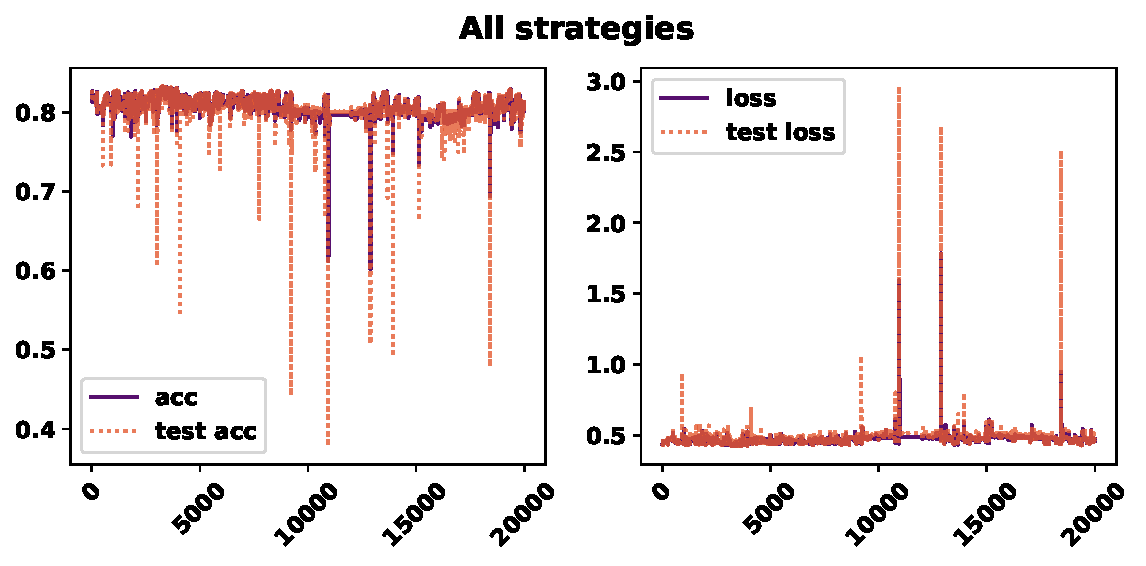
\includegraphics[width=.8\textwidth]{src/chapters/07/img/validation_plot_all_strategies.pdf}
    \end{subfigure}\hfill
    \begin{subfigure}{\textwidth}
    \centering
    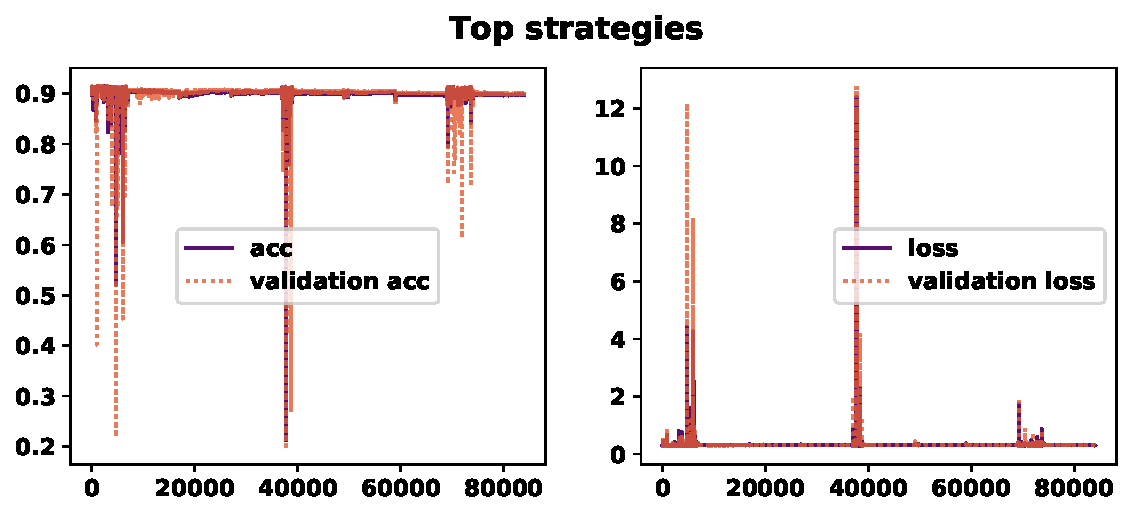
\includegraphics[width=.8\textwidth]{src/chapters/07/img/validation_plot_top_strategies.pdf}
    \end{subfigure}
    \begin{subfigure}{\textwidth}
    \centering
    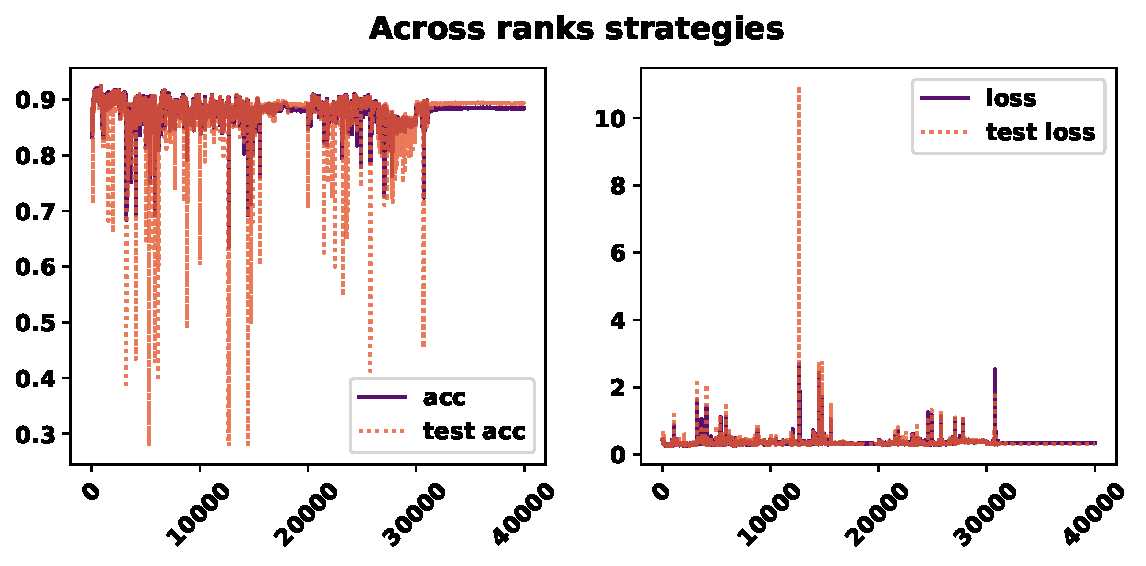
\includegraphics[width=.8\textwidth]{src/chapters/07/img/validation_plot_across_ranks_strategies.pdf}
    \end{subfigure}
    \begin{subfigure}{\textwidth}
    \centering
    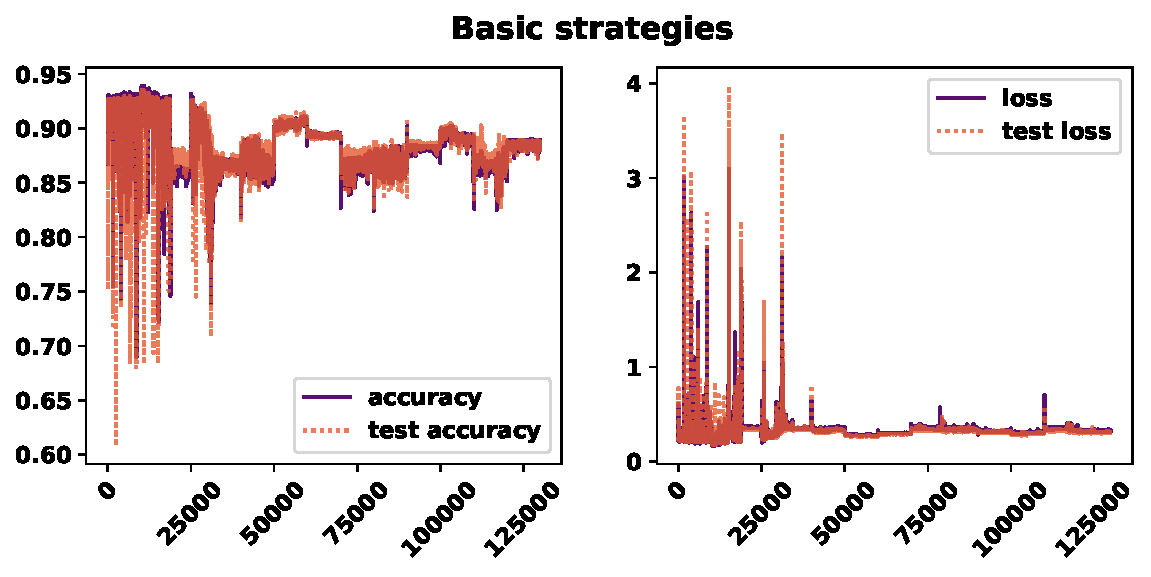
\includegraphics[width=.8\textwidth]{src/chapters/07/img/validation_plot_basic_strategies.pdf}
    \end{subfigure}
    \caption{Loss function and accuracy of the networks based on the StoS network,
    over the number of epochs.}\label{fig:validation_sequence_to_sequence}
\end{figure}

For the StoP networks there appears to be more variation in the test loss and
accuracy, Figure~\ref{fig:validation_sequence_to_probability}. This is more evident
for the networks that were trained on the top strategies and the strategies
across ranks. This could indicate that the networks are overfitting. The StoP
network trained on the entire training data set has managed to maintained
a low loss value (at 0.5) and a training accuracy of 0.75. The most successfully
trained StoP network appears to be the network trained on the basic strategies.

\begin{figure}[!htbp]
    \begin{subfigure}{\textwidth}
    \centering
    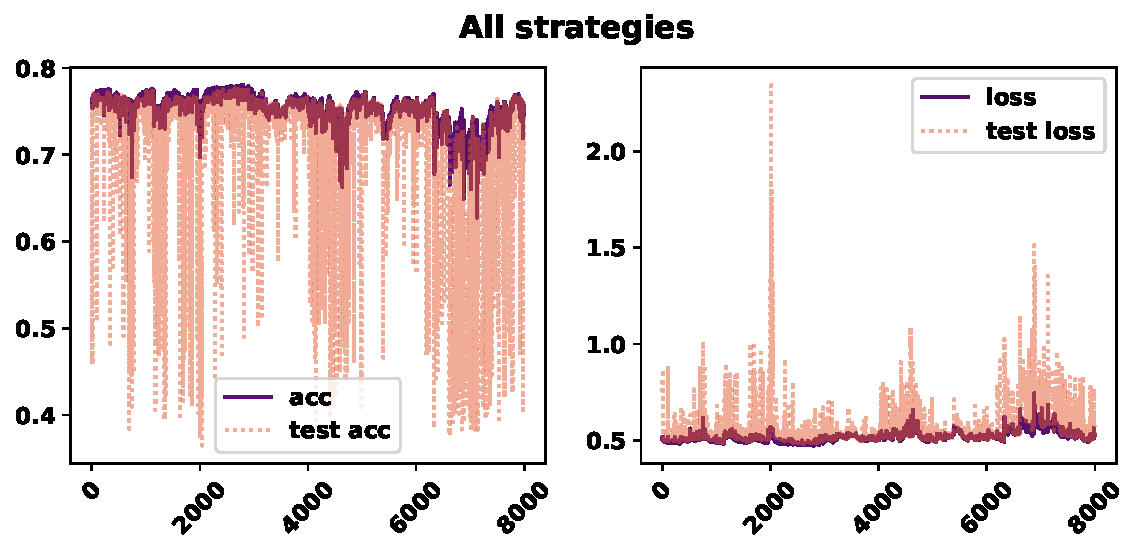
\includegraphics[width=.8\textwidth]{src/chapters/07/img/validation_plot_classification_all_strategies.pdf}
    \end{subfigure}\hfill
    \begin{subfigure}{\textwidth}
    \centering
    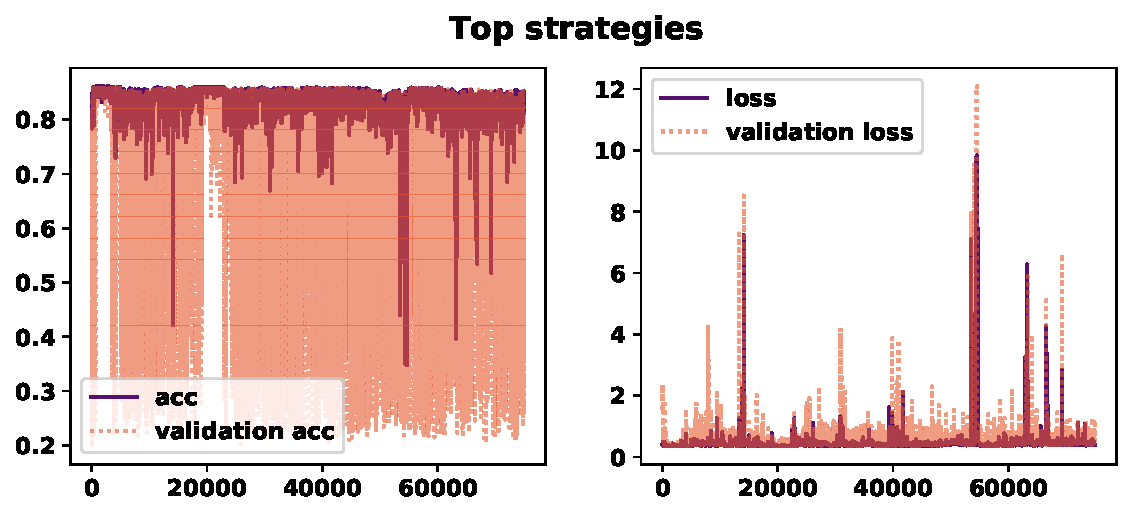
\includegraphics[width=.8\textwidth]{src/chapters/07/img/validation_plot_classification_top_strategies.pdf}
    \end{subfigure}
    \begin{subfigure}{\textwidth}
    \centering
    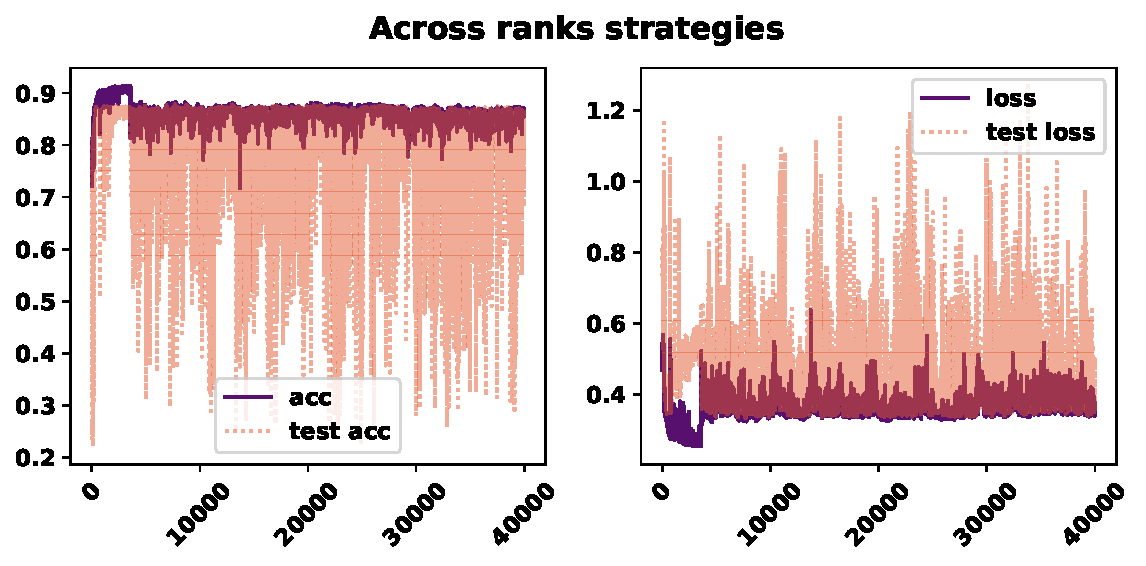
\includegraphics[width=.8\textwidth]{src/chapters/07/img/validation_plot_classification_across_ranks_strategies.pdf}
    \end{subfigure}
    \begin{subfigure}{\textwidth}
    \centering
    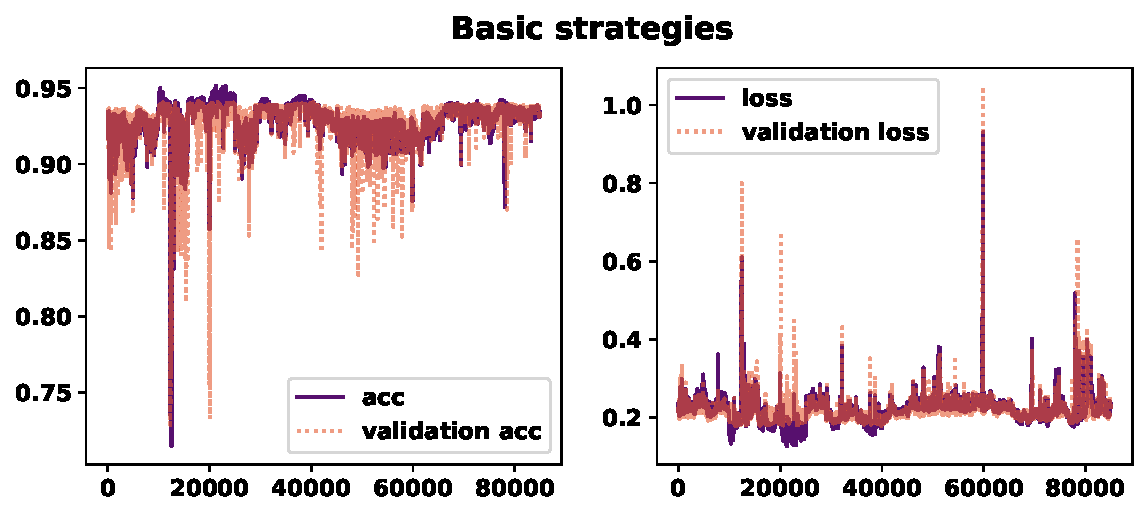
\includegraphics[width=.8\textwidth]{src/chapters/07/img/validation_plot_classification_basic_strategies.pdf}
    \end{subfigure}
    \caption{Loss function and accuracy of the networks based on the StoP
    network, over the number of epochs.}\label{fig:validation_sequence_to_probability}
\end{figure}

This section has presented the \lstmnetworks trained LSTM networks of this thesis.
These networks are based on two different architectures and have been trained
on four different training data sets. The networks' validation based on the
training data sets was presented in this section. In the next section the networks
are evaluated as IPD strategies.

\section{Validation of LSTM based strategies using a meta tournament analysis}\label{section:rnn_strategy_validation}

This section evaluates the trained LSTM networks as IPD strategies.
A strategy class called the \mintinline{python}{LSTMPlayer} was implemented
in order for the networks, which are Keras models, to interact in an IPD match
simulated with APL. The source code for the \mintinline{python}{LSTMPlayer} is
given by Figure~\ref{fig:lstm_player_source_code}. The class has three input
arguments:

\begin{itemize}
    \item A Keras model. The input models are the \lstmnetworks trained LSTM networks
    presented in section~\ref{section:training_a_rnn}.
    \item A reshape history function. A function that reshapes the opponent's
    history to the appropriate LSTM input.
    \item The probability that the strategy opens with cooperation on the first turn denoted
    as \(p_o\). The LSTM networks can be used to predict the strategy's next
    action following the opponent's opening turn. Thus, the strategy's opening
    action must be manually defined.
\end{itemize}

Following the opening turn the LSTM strategy makes a prediction based on the
opponent's history. The strategy has an infinite memory because it needs to
remember all the actions made by the opponent. The prediction of the networks
correspond to the probability of cooperating. The LSTM strategy makes a deterministic
decision based on the predicted probability. It cooperates if the prediction
on the last time step is greater than 0.5, otherwise it defects.
In Section~\ref{sec:stochastic-lstm-strategies} the performance of strategy that
plays stochastically will be briefly discussed.

\begin{figure}[!htbp]
\begin{sourcepy}
import numpy as np

import axelrod as axl
from axelrod.random_ import random_choice
from keras.layers import LSTM, Dense, Dropout
from keras.models import Sequential

C, D = axl.Action.C, axl.Action.D


class LSTMPlayer(axl.Player):
    name = "The LSTM player"
    classifier = {
        "memory_depth": float("inf"),
        "stochastic": True,
        "inspects_source": False,
        "manipulates_source": False,
        "manipulates_state": False,
    }

    def __init__(self, model, reshape_history_funct, opening_probability=0.78):
        self.model = model
        self.opening_probability = opening_probability
        self.reshape_history_function = reshape_history_funct
        super().__init__()
        if opening_probability in [0, 1]:
            self.classifier["stochastic"] = False

    def strategy(self, opponent):
        if len(self.history) == 0:
            return random_choice(self.opening_probability)

        history = [action.value for action in opponent.history]
        prediction = float(
            self.model.predict(self.reshape_history_function(history))[0][-1]
        )

        return axl.Action(round(prediction))

    def __repr__(self):
        return self.name
\end{sourcepy}
\caption{Implementation of the \mintinline{python}{LSTMPlayer} class.}\label{fig:lstm_player_source_code}
\end{figure}

The \lstmnetworks trained LSTM networks are used to introduce \lstmstrategies
new IPD strategies. Each network corresponds to three distinct players with a
different opening move. More specifically, three different values of \(p_o\) are
used here. These are \(p_o = 0\), \(p_o = 1\) and \(p_o = 0.78\). The
probability 0.78 is the probability that the best response sequences of Chapter
\ref{chapter:best_response_sequence} opens with a cooperation. Thus, a total of
\(8 \times 3 =  \lstmstrategies\) IPD strategies are evaluated in this section.

The performance of the LSTM strategies are evaluated and compared in
\metatournamentslstm standard tournaments similarly to Chapter~\ref{chapter:meta_tournaments}. The process of collecting the
tournaments results for each strategy is given by
Algorithm~\ref{algorithm:meta_tournament_lstm_validation}.

\begin{algorithm}[!htbp]
    \setstretch{1.35}
    \ForEach{\text{seed} $\in [0, 300]$}{
        $s \gets \text{randomly select integer}\in [s_{min}, s_{max}]$\;
        $\text{players} \gets  \text{randomly select $s$ players}$\;
        $\text{players} \gets  \text{players} + \text{LSTM strategy}$\;
        $s \gets s + 1$\;
        $k \gets  50$\;
        $n \gets  200$\;
        \vspace{0.4cm}
        $\text{result standard}$ $\gets$ Axelrod.tournament$(\text{players}, n, k)$\;}
    \KwRet{result standard}\;
    \caption{Standard tournament result summary collection algorithm}
    \label{algorithm:meta_tournament_lstm_validation}
\end{algorithm}

For each trial a random size \(s \in [5, 10]\) is selected, and from the
\numberofstrategiesbestsequences strategies of Appendix, a random list of \(s\) strategies is chosen. %TODO fix Appendix of Chapter 6.
The LSTM player is then added
to the list of players, increasing the size to \(s + 1\). For the given list of
strategies a standard tournament of 200 turns is performed and repeated 50
times. The number of turns is fixed at 200. In
Chapter~\ref{chapter:best_response_sequence} the sequences were fixed to 205
turns which resulted in many best response sequences to defect on the last turn
as the match was coming to an end. To avoid a series of 
unconditional defections by the LSTM strategies their performance is evaluated
in  200 turns, which is a common number of turns used in the IPD literature~\cite{Axelrod1980a, Axelrod1980b, Harper2017, Knight2016}.

A total of \metatournamentslstm trials of
Algorithm~\ref{algorithm:meta_tournament_lstm_validation} have been run. For
each trial a result summary (in the format of Table~\ref{table:output_result})
is exported. Similarly to Chapter~\ref{chapter:meta_tournaments}, the performance of the strategies is evaluated on the normalised.
rank \(r\), and more specifically on the median normalised rank \(\bar{r}\). As
a reminder \(r\) is calculated as a strategy's rank divided by \(s-1\).

The \(\bar{r}\) of each of the \lstmstrategies strategies over the \metatournamentslstm
standard tournaments is given by Table~\ref{table:normalised_rank_lstm_tournaments}.

\begin{table}[!htbp]
    \begin{center}
    \resizebox{.9\textwidth}{!}{
        \begin{tabular}{lllllll}
\toprule
{} & \multicolumn{3}{c}{\textbf{sequence to sequence}} & \multicolumn{3}{c}{\textbf{sequence to probability}} \\
{} &                       $p_o=0$ &                       $p_o=1$ &                    $p_o=0.78$ &                       $p_o=0$ &                       $p_o=1$ &                    $p_o=0.78$ \\
\midrule
All strategies          &  \cellcolor{orange!67.0}0.667 &  \cellcolor{orange!22.0}0.222 &  \cellcolor{orange!33.0}0.333 &  \cellcolor{orange!78.0}0.778 &  \cellcolor{orange!33.0}0.333 &    \cellcolor{orange!50.0}0.500 \\
Top strategies          &  \cellcolor{orange!71.0}0.714 &  \cellcolor{orange!44.0}0.444 &    \cellcolor{orange!50.0}0.500 &    \cellcolor{orange!50.0}0.500 &  \cellcolor{orange!43.0}0.429 &  \cellcolor{orange!43.0}0.429 \\
Across ranks strategies &   \cellcolor{orange!75.0}0.750 &  \cellcolor{orange!67.0}0.667 &  \cellcolor{orange!68.0}0.683 &    \cellcolor{orange!50.0}0.500 &   \cellcolor{orange!25.0}0.250 &    \cellcolor{orange!30.0}0.300 \\
Basic strategies        &    \cellcolor{orange!80.0}0.800 &    \cellcolor{orange!60.0}0.600 &  \cellcolor{orange!62.0}0.625 &    \cellcolor{orange!80.0}0.800 &    \cellcolor{orange!30.0}0.300 &  \cellcolor{orange!43.0}0.429 \\
\bottomrule
\end{tabular}

    }
\end{center}
\caption{The median normalised ranks of the 24 LSTM strategies over the standard
tournaments. A \(\bar{r}\) closer to 0 indicates a more successful performance.}
\label{table:normalised_rank_lstm_tournaments}
\end{table}

The strategy with the lowest \(\bar{r}\) over the \metatournamentslstm
tournaments is the LSTM strategy based on the StoS network trained over the entire
training set with \(p_o=1\). The strategy achieved a \(\bar{r}\) of 0.222. The
second most successful performance is by the StoP based strategy trained against
the across the ranks strategies with \(p_o=1\). In
section~\ref{section:training_a_rnn} it was indicated that the specific network
was overfitting, however, as an IPD strategy the network outperforms any other
StoP strategies.

A few strategies have achieved a \(\bar{r}\)
close to 0.3. These include the StoS strategy trained on the entire data set
with \(p_o=0.78\), and the StoP strategies trained against all strategies,
across the ranks strategies, and against the basic strategies with \(p_o=1\),
\(p_o=0.78\) and \(p_o=1\) equivalently.

The LSTM strategies that open with cooperation outperform any other strategy,
based on the same LSTM networks. Overall, the best performing
strategies open with cooperation. The strategies that open with a probabilistic
cooperation perform better than the strategies that open with defection.
Interestedly, from Table~\ref{table:normalised_rank_lstm_tournaments} it is
indicated that the strategies trained on the subsets perform better when they
are based on the StoP model. There is no intuition as to why that is. The
StoP networks have more learning parameters and yet they perform better when
trained on the smaller training sets than the StoS network. The StoP
network, trained against the entire data set, has trained for the smallest
number of epochs. A topic of future work would be to train the specific network
for more epochs.

Figure~\ref{fig:normalised_rank_distributions_sequence_to_sequence} gives the
\(r\) distributions for the strategies based on the StoS network. All the
distributions for \(p_o=0\) have a median higher than 0.66, indicating that
those strategies on average perform in the bottom half of a tournament. The most
successful strategy is the strategy trained against all strategies with
\(p_o=1\). The strategy's distribution shows that the strategy ranked highly in
most of the tournament it participated with only a few exceptions. Even if when
\(p_o\) is lowered to 0.78 the strategy still performs adequately. The rest
of the distributions appear to have peaks either at 0.5 or closer to 1. A
statistical summary of the distributions are given by
Table~\ref{table:statistic_summary_s_to_s}.

\begin{figure}[!htbp]
    \begin{subfigure}{\textwidth}
    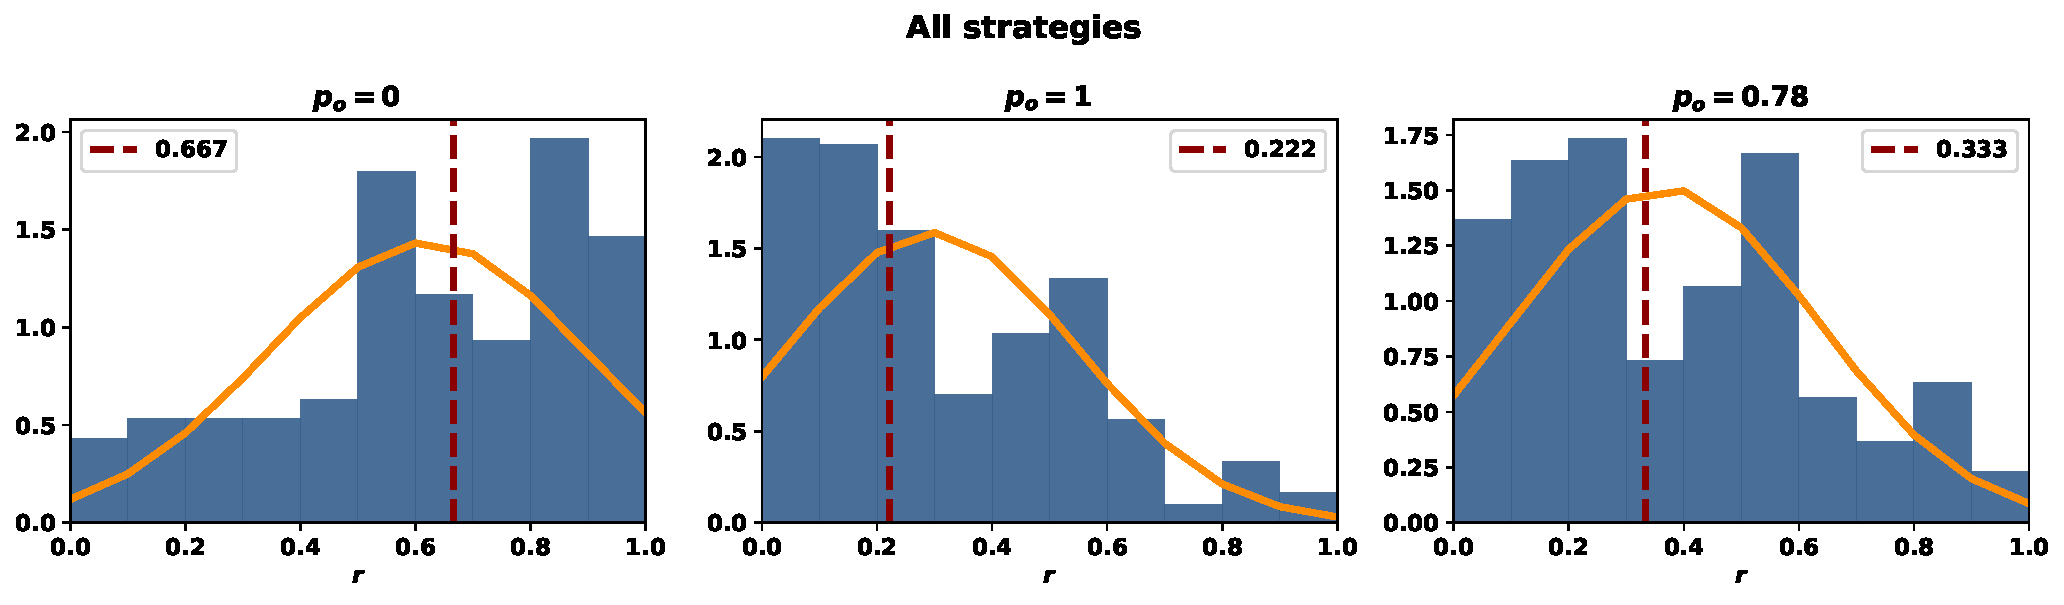
\includegraphics[width=\textwidth]{src/chapters/07/img/normalised_rank_all_strategies.pdf}
    \end{subfigure}
    \par\bigskip
    \begin{subfigure}{\textwidth}
    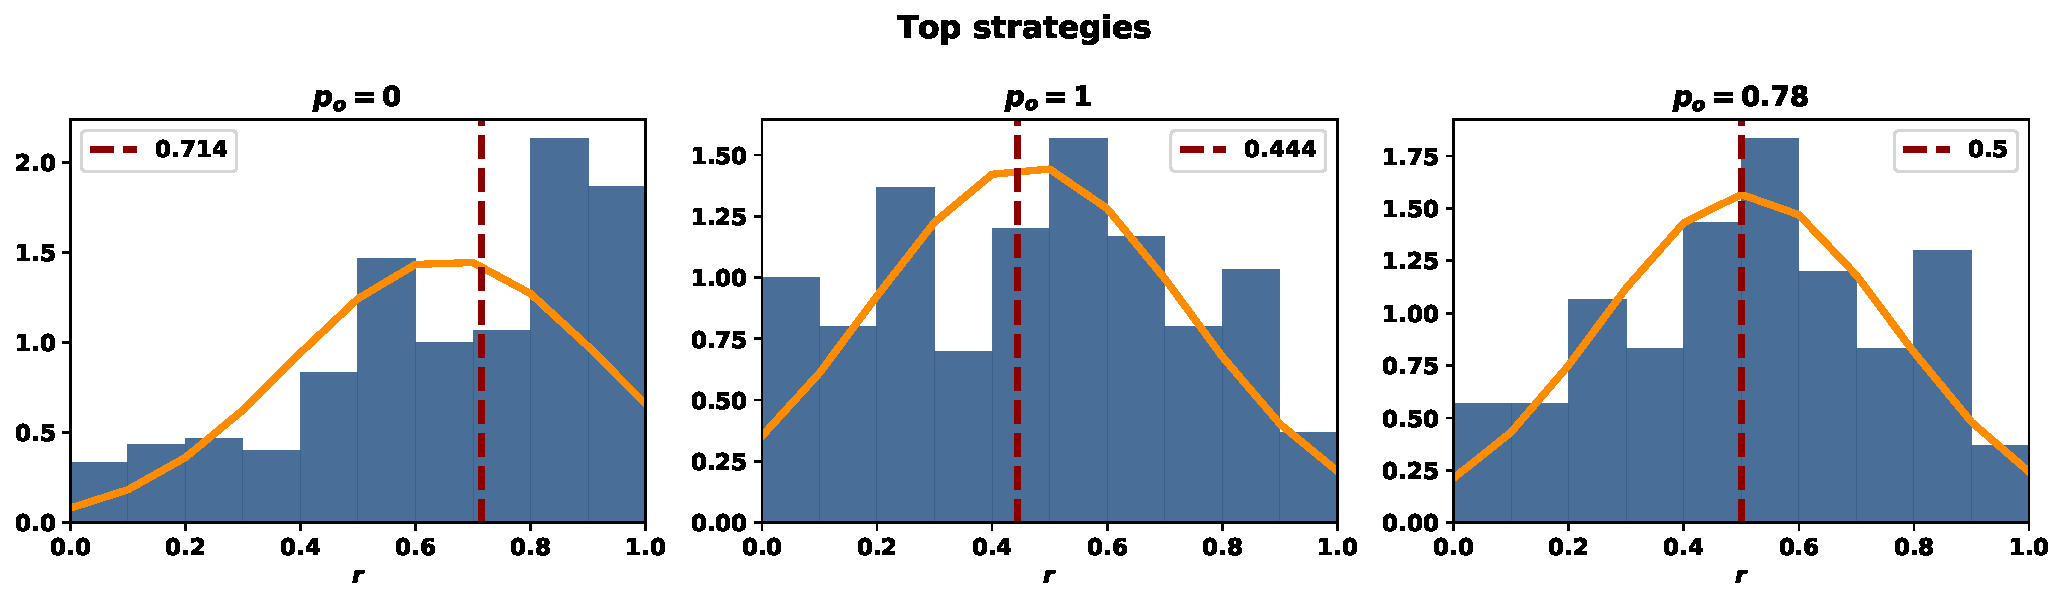
\includegraphics[width=\textwidth]{src/chapters/07/img/normalised_rank_top_strategies.pdf}
    \end{subfigure}
    \par\bigskip
    \begin{subfigure}{\textwidth}
    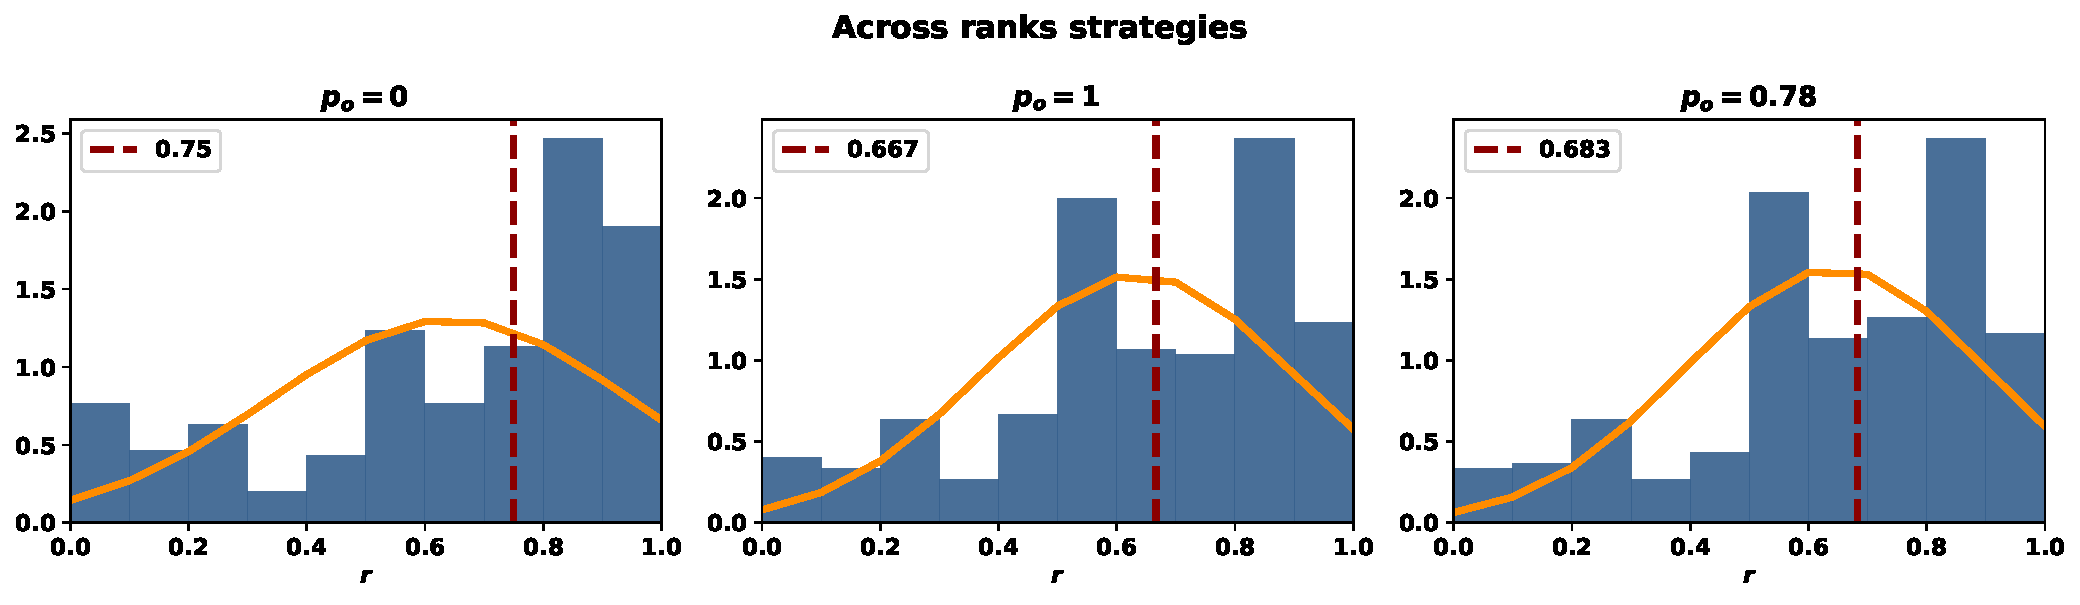
\includegraphics[width=\textwidth]{src/chapters/07/img/normalised_rank_across_ranks_strategies.pdf}
    \end{subfigure}
    \par\bigskip
    \begin{subfigure}{\textwidth}
    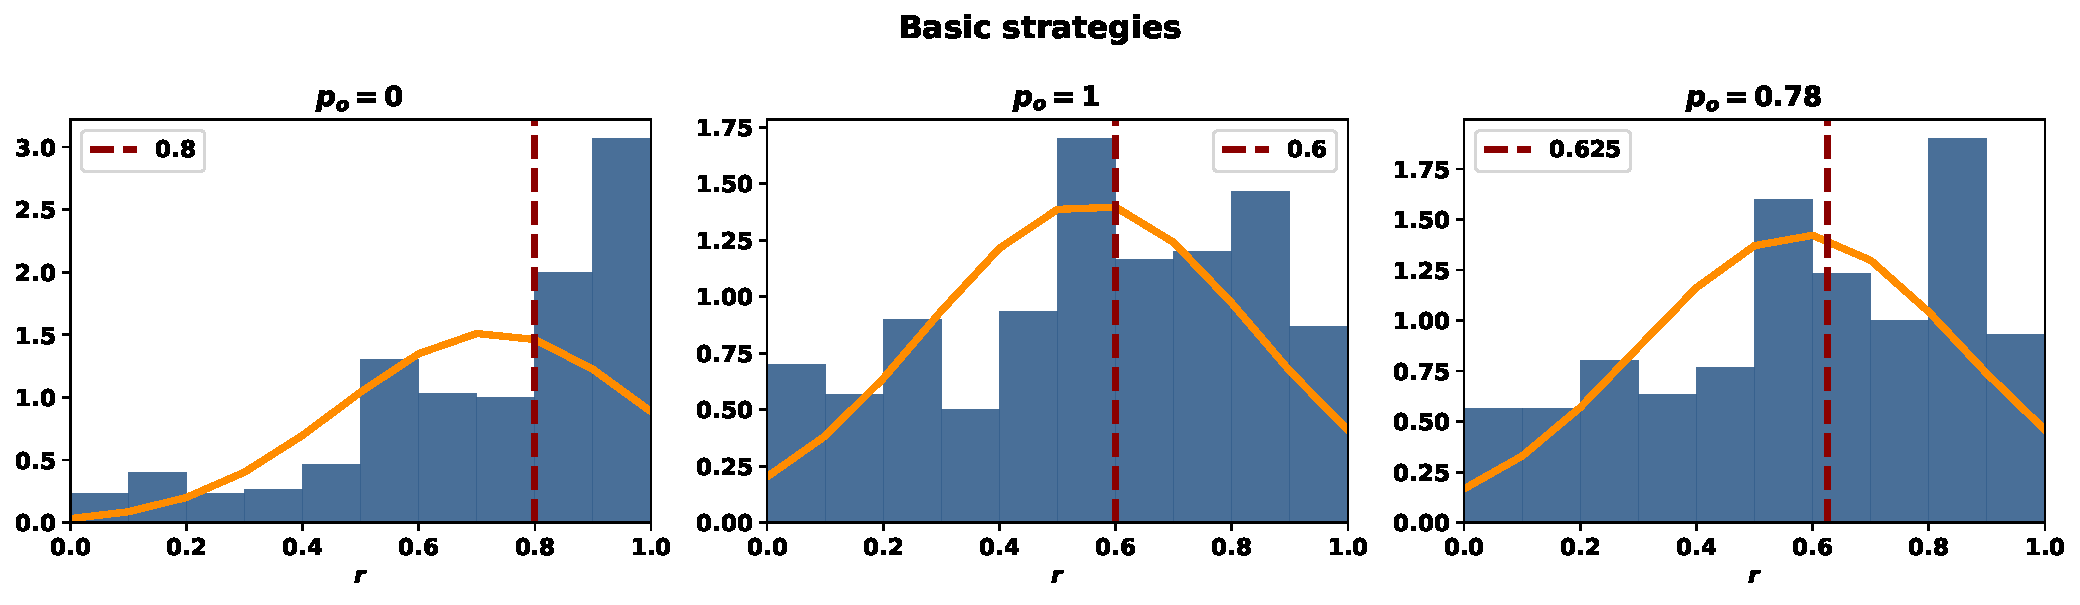
\includegraphics[width=\textwidth]{src/chapters/07/img/normalised_rank_basic_strategies.pdf}
    \end{subfigure}
    \caption{Normalised rank distributions for the strategies which are based on the StoS
    LSTM.}\label{fig:normalised_rank_distributions_sequence_to_sequence}
\end{figure}

\begin{table}[!htbp]
    \begin{center}
    \resizebox{\textwidth}{!}{
        \begin{tabular}{llrrrrrrrrrrrr}
\toprule
                 &            &  count &   mean &    std &  min &    10\% &    25\% &    50\% &    75\% &    95\% &  max &   skew &   kurt \\
\midrule
\rowcolor{Gray}
All strategies & $p_o=0$ &  300.0 &  0.620 &  0.278 &  0.0 &  0.200 &  0.429 &  0.667 &  0.839 &  1.000 &  1.0 & -0.523 & -0.587 \\
\rowcolor{Gray}
                 & $p_o=1$ &  300.0 &  0.295 &  0.252 &  0.0 &  0.000 &  0.111 &  0.222 &  0.458 &  0.779 &  1.0 &  0.702 & -0.251 \\
\rowcolor{Gray}
                 & $p_o=0.78$ &  300.0 &  0.368 &  0.265 &  0.0 &  0.000 &  0.143 &  0.333 &  0.560 &  0.833 &  1.0 &  0.433 & -0.647 \\
                 \midrule
Top strategies & $p_o=0$ &  300.0 &  0.655 &  0.273 &  0.0 &  0.250 &  0.500 &  0.714 &  0.875 &  1.000 &  1.0 & -0.629 & -0.436 \\
                 & $p_o=1$ &  300.0 &  0.461 &  0.274 &  0.0 &  0.090 &  0.222 &  0.444 &  0.667 &  0.875 &  1.0 & -0.029 & -0.940 \\
                 & $p_o=0.78$ &  300.0 &  0.509 &  0.255 &  0.0 &  0.167 &  0.333 &  0.500 &  0.704 &  0.876 &  1.0 & -0.158 & -0.710 \\
                 \midrule
\rowcolor{Gray}
Representative strategies & $p_o=0$ &  300.0 &  0.643 &  0.306 &  0.0 &  0.141 &  0.486 &  0.750 &  0.875 &  1.000 &  1.0 & -0.768 & -0.523 \\
\rowcolor{Gray}
                 & $p_o=1$ &  300.0 &  0.636 &  0.262 &  0.0 &  0.250 &  0.500 &  0.667 &  0.833 &  1.000 &  1.0 & -0.680 & -0.198 \\
\rowcolor{Gray}
                 & $p_o=0.78$ &  300.0 &  0.645 &  0.255 &  0.0 &  0.250 &  0.500 &  0.683 &  0.833 &  1.000 &  1.0 & -0.754 & -0.034 \\
                 \midrule
Basic strategies & $p_o=0$ &  300.0 &  0.728 &  0.263 &  0.0 &  0.333 &  0.600 &  0.800 &  1.000 &  1.000 &  1.0 & -0.949 &  0.229 \\
                 & $p_o=1$ &  300.0 &  0.556 &  0.283 &  0.0 &  0.143 &  0.375 &  0.600 &  0.778 &  1.000 &  1.0 & -0.365 & -0.803 \\
                 & $p_o=0.78$ &  300.0 &  0.579 &  0.280 &  0.0 &  0.167 &  0.375 &  0.625 &  0.800 &  1.000 &  1.0 & -0.435 & -0.772 \\
\bottomrule
\end{tabular}

    }
\end{center}
\caption{Statistics summary of the \(r\) distributions for the strategies
based on the StoS network.}\label{table:statistic_summary_s_to_s}
\end{table}

Figure~\ref{fig:normalised_rank_distributions_sequence_to_probability} gives the
\(r\) distributions for the strategies based on the StoP network. For \(p_o=0\)
the performance of the strategies remains poorly. The strategies that have been
trained against all strategies, across the ranks and basic strategies with
\(p_o=1\) appear to have won several of the tournaments they
participated in. The statistics summary of the distributions is given by
Table~\ref{table:statistic_summary_s_to_p}.

\begin{figure}[!htbp]
    \begin{subfigure}{\textwidth}
    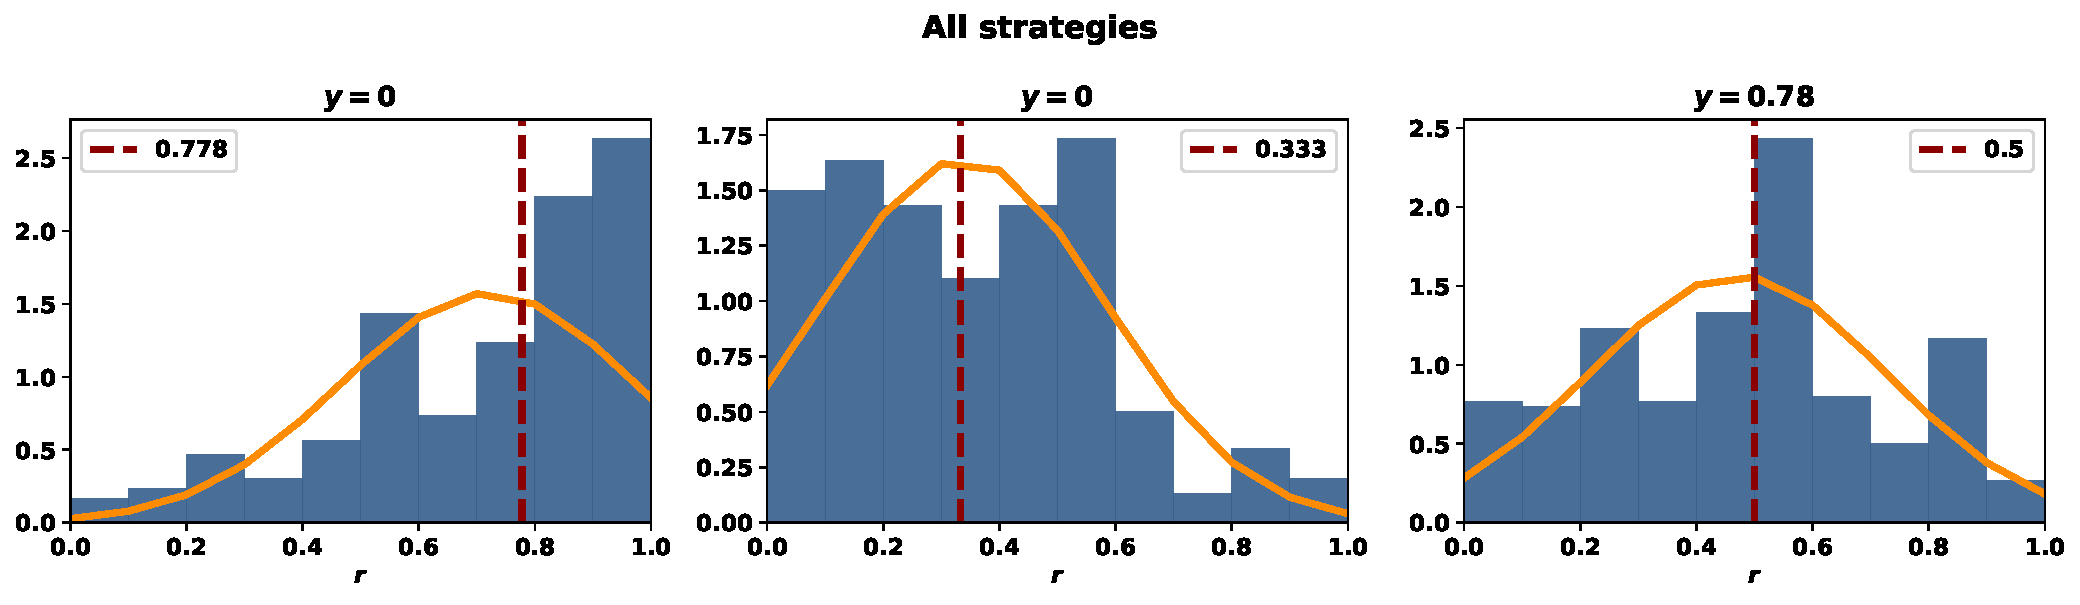
\includegraphics[width=\textwidth]{src/chapters/07/img/normalised_rank_classification_all_strategies.pdf}
    \end{subfigure}
    \par\bigskip
    \begin{subfigure}{\textwidth}
    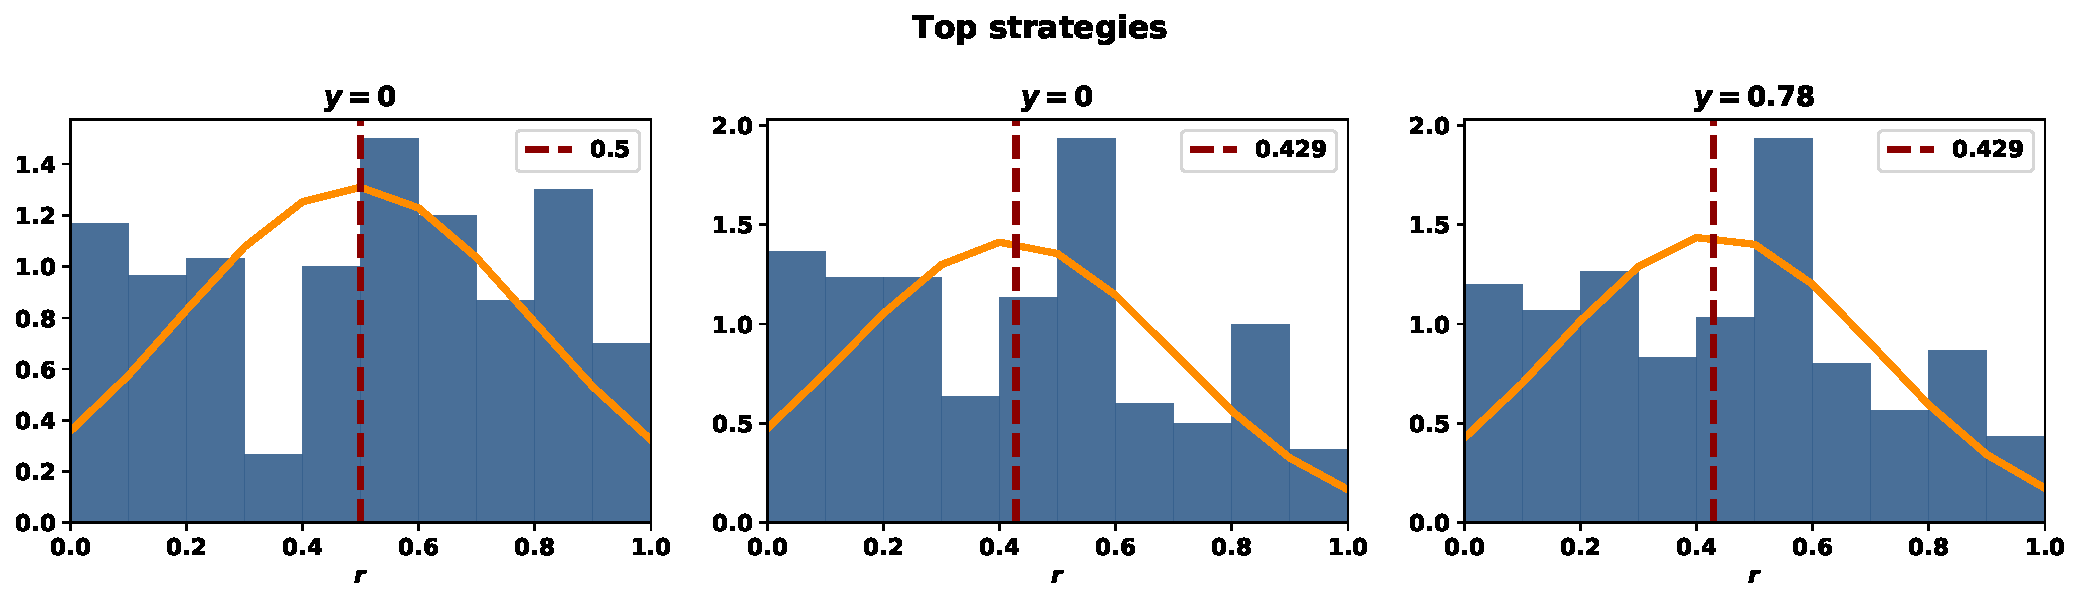
\includegraphics[width=\textwidth]{src/chapters/07/img/normalised_rank_classification_top_strategies.pdf}
    \end{subfigure}
    \par\bigskip
    \begin{subfigure}{\textwidth}
    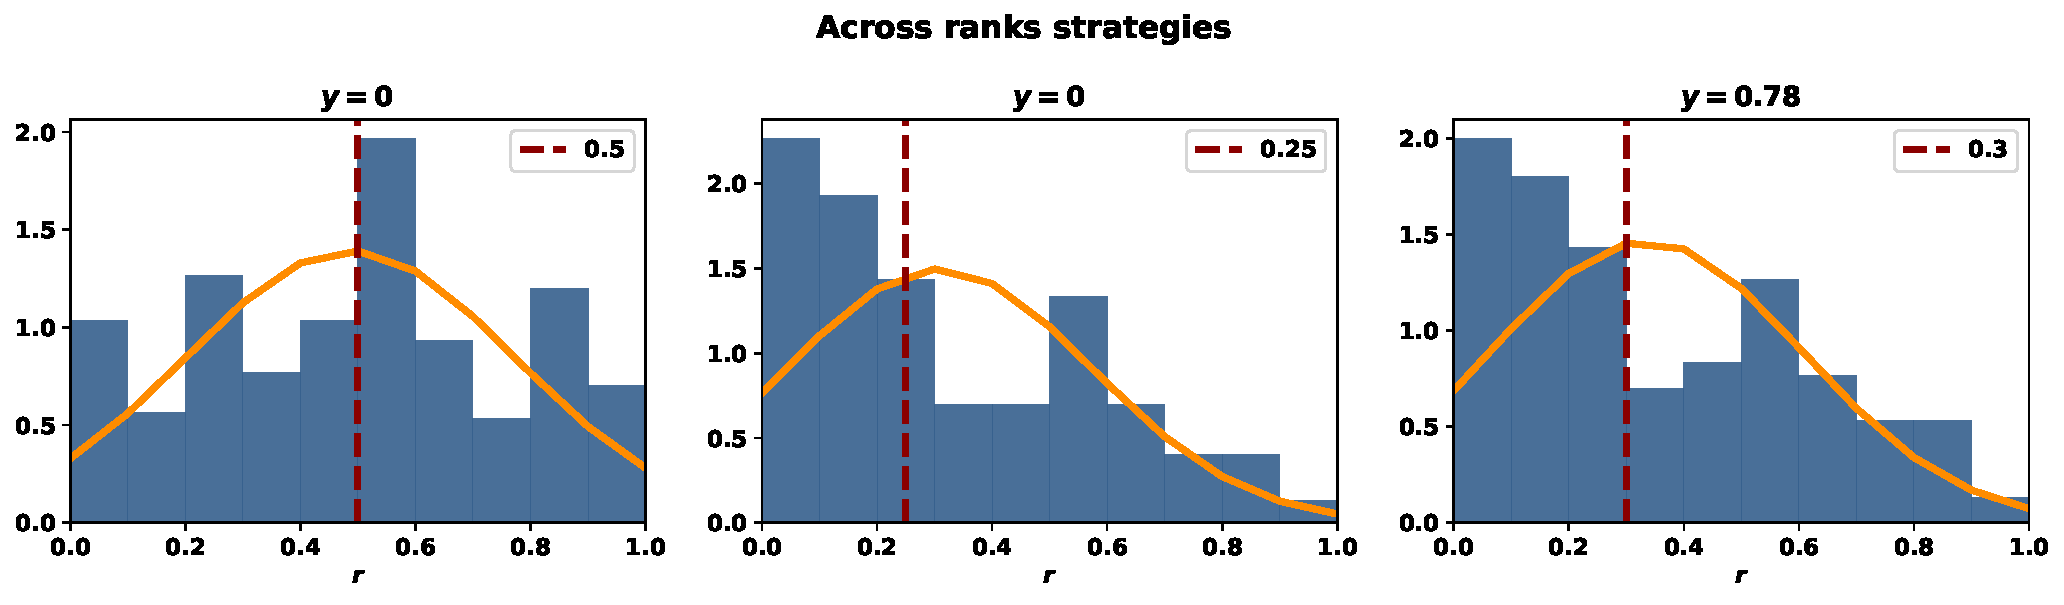
\includegraphics[width=\textwidth]{src/chapters/07/img/normalised_rank_classification_across_ranks_strategies.pdf}
    \end{subfigure}
    \par\bigskip
    \begin{subfigure}{\textwidth}
    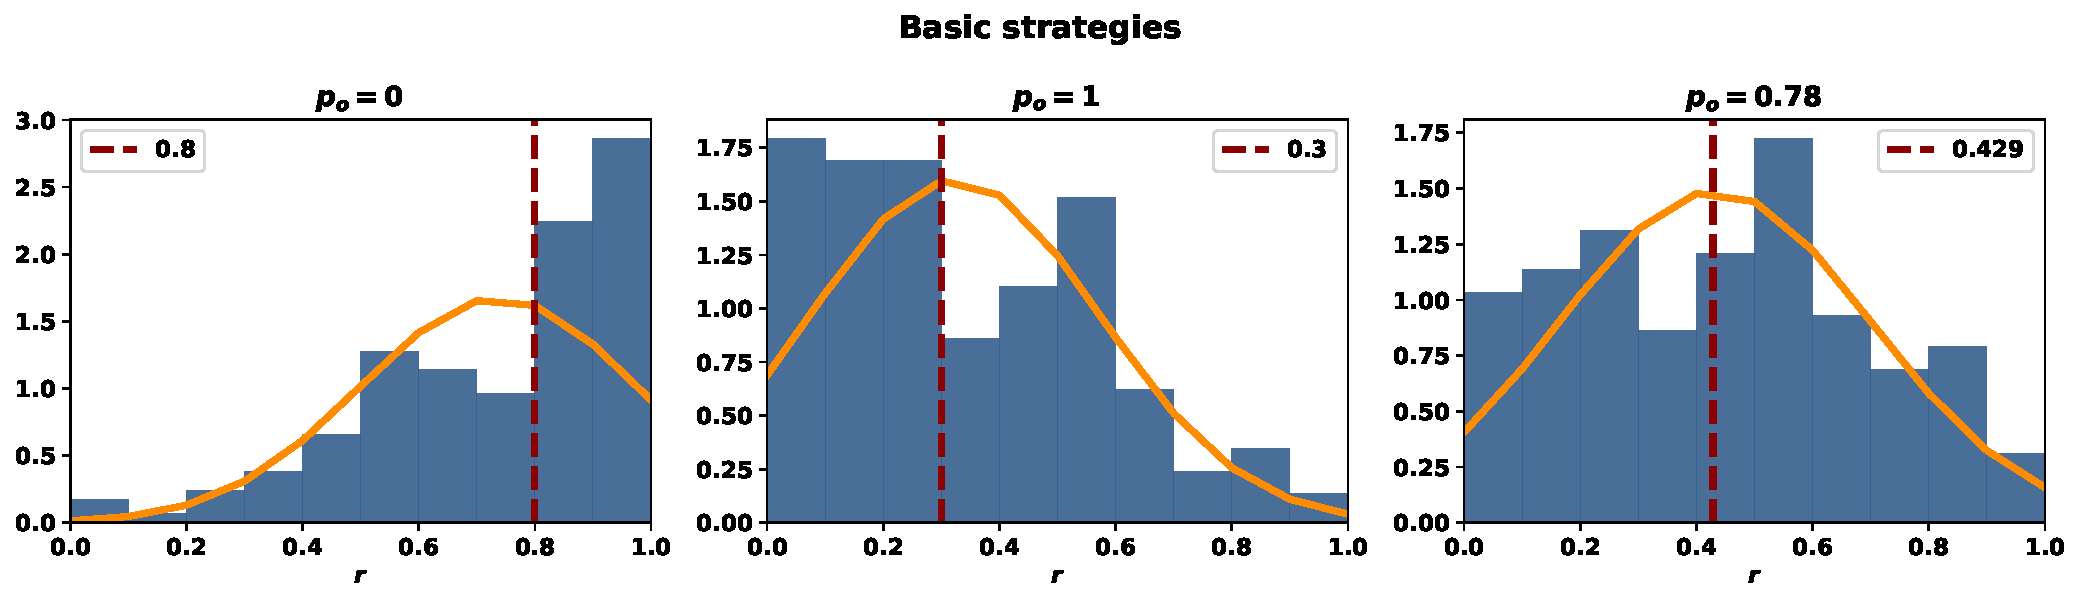
\includegraphics[width=\textwidth]{src/chapters/07/img/normalised_rank_classification_basic_strategies.pdf}
    \end{subfigure}
    \caption{Normalised rank distributions for the strategies which are based on the StoP
    LSTM.}\label{fig:normalised_rank_distributions_sequence_to_probability}
\end{figure}

\begin{table}[!htbp]
    \begin{center}
    \resizebox{.9\textwidth}{!}{
        \begin{tabular}{llrrrrrrrrrrrr}
\toprule
                 &            &  count &   mean &    std &  min &    10\% &    25\% &    50\% &    75\% &    95\% &  max &   skew &   kurt \\
\midrule
\rowcolor{Gray}
All strategies & $p_o=0$ &  300.0 &  0.720 &  0.254 &  0.0 &  0.333 &  0.571 &  0.778 &  0.900 &  1.000 &  1.0 & -0.860 &  0.056 \\
\rowcolor{Gray}
                 & $p_o=1$ &  300.0 &  0.339 &  0.244 &  0.0 &  0.000 &  0.125 &  0.333 &  0.500 &  0.800 &  1.0 &  0.458 & -0.280 \\
\rowcolor{Gray}
                 & $p_o=0.78$ &  300.0 &  0.471 &  0.255 &  0.0 &  0.125 &  0.286 &  0.500 &  0.625 &  0.875 &  1.0 & -0.064 & -0.696 \\
                 \midrule
Top strategies & $p_o=0$ &  300.0 &  0.491 &  0.305 &  0.0 &  0.000 &  0.200 &  0.500 &  0.714 &  1.000 &  1.0 & -0.131 & -1.140 \\
                 & $p_o=1$ &  300.0 &  0.417 &  0.283 &  0.0 &  0.000 &  0.167 &  0.429 &  0.600 &  0.875 &  1.0 &  0.157 & -0.974 \\
                 & $p_o=0.78$ &  300.0 &  0.432 &  0.277 &  0.0 &  0.000 &  0.200 &  0.429 &  0.625 &  0.876 &  1.0 &  0.109 & -0.891 \\
                 \midrule
\rowcolor{Gray}
Across ranks strategies & $p_o=0$ &  300.0 &  0.487 &  0.287 &  0.0 &  0.000 &  0.286 &  0.500 &  0.700 &  1.000 &  1.0 & -0.037 & -0.899 \\
\rowcolor{Gray}
                 & $p_o=1$ &  300.0 &  0.308 &  0.267 &  0.0 &  0.000 &  0.111 &  0.250 &  0.500 &  0.800 &  1.0 &  0.586 & -0.695 \\
\rowcolor{Gray}
                 & $p_o=0.78$ &  300.0 &  0.335 &  0.272 &  0.0 &  0.000 &  0.125 &  0.300 &  0.556 &  0.800 &  1.0 &  0.465 & -0.867 \\
                 \midrule
Basic strategies & $p_o=0$ &  290.0 &  0.738 &  0.239 &  0.0 &  0.400 &  0.600 &  0.800 &  0.975 &  1.000 &  1.0 & -0.881 &  0.315 \\
                 & $p_o=1$ &  290.0 &  0.323 &  0.249 &  0.0 &  0.000 &  0.125 &  0.300 &  0.500 &  0.778 &  1.0 &  0.491 & -0.535 \\
                 & $p_o=0.78$ &  290.0 &  0.432 &  0.269 &  0.0 &  0.000 &  0.200 &  0.429 &  0.625 &  0.875 &  1.0 &  0.096 & -0.916 \\
\bottomrule
\end{tabular}

    }
\end{center}
\caption{Statistics summary of the \(r\) distributions for the strategies
based on the StoP network.}\label{table:statistic_summary_s_to_p}
\end{table}

An interesting question that arises is: what is the probability that a LSTM
strategy ranks in the top half of a standard tournament?

This is answered by calculating the cumulative distribution function (CFD) of
\(r\). CFD is the cumulative probability for a given value. It can be used to
determine the probability that a random observation taken from the population
will be less than or equal to a certain value. The CFD distributions are shown by
Figures~\ref{fig:cfd_s_to_s}-\ref{fig:cfd_s_to_p}. The demonstrate that the the
strategies with a \(\bar{r}\) less than 0.333 have a 0.70-0.80 probability of
being on the top ranks on a standard IPD tournament.

\begin{figure}[!htbp]
    \begin{subfigure}{.45\textwidth}
    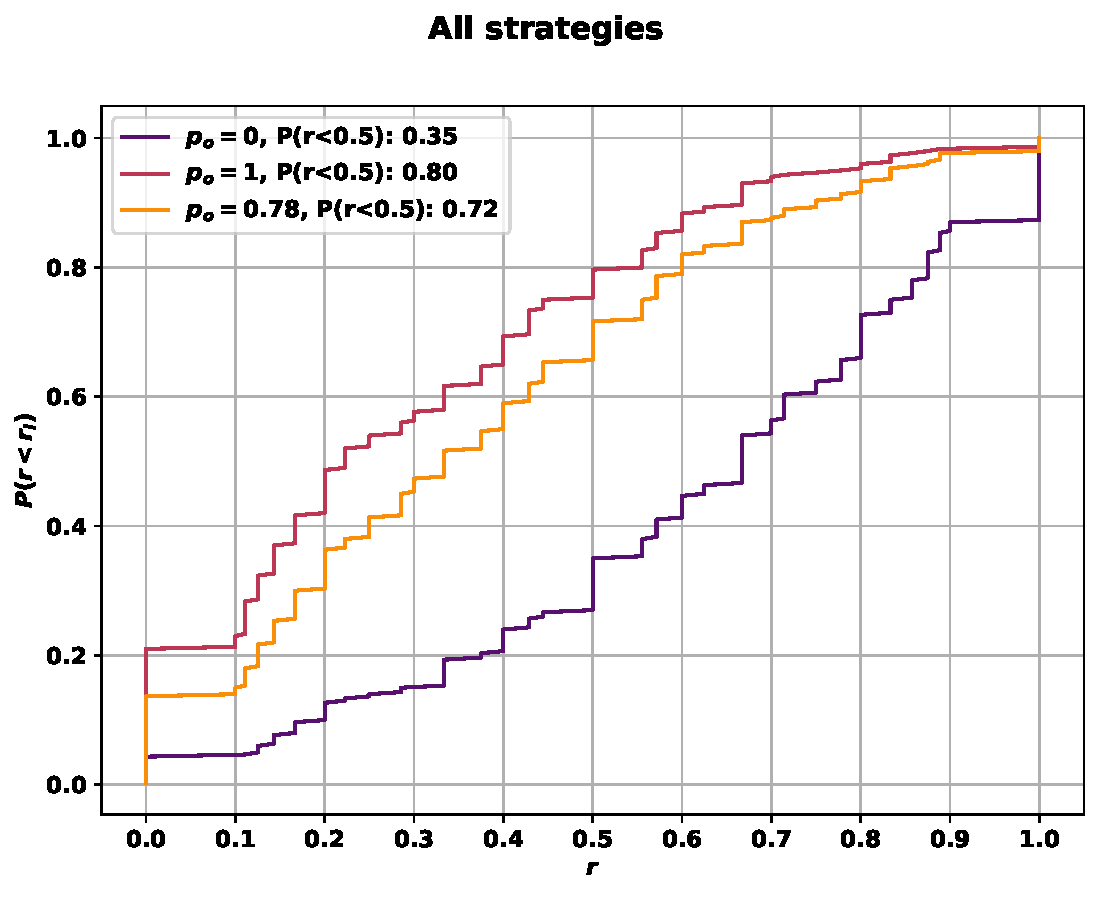
\includegraphics[width=\textwidth]{src/chapters/07/img/cfd_to_sequence_all_strategies.pdf}
    \end{subfigure}\hfill
    \begin{subfigure}{.45\textwidth}
    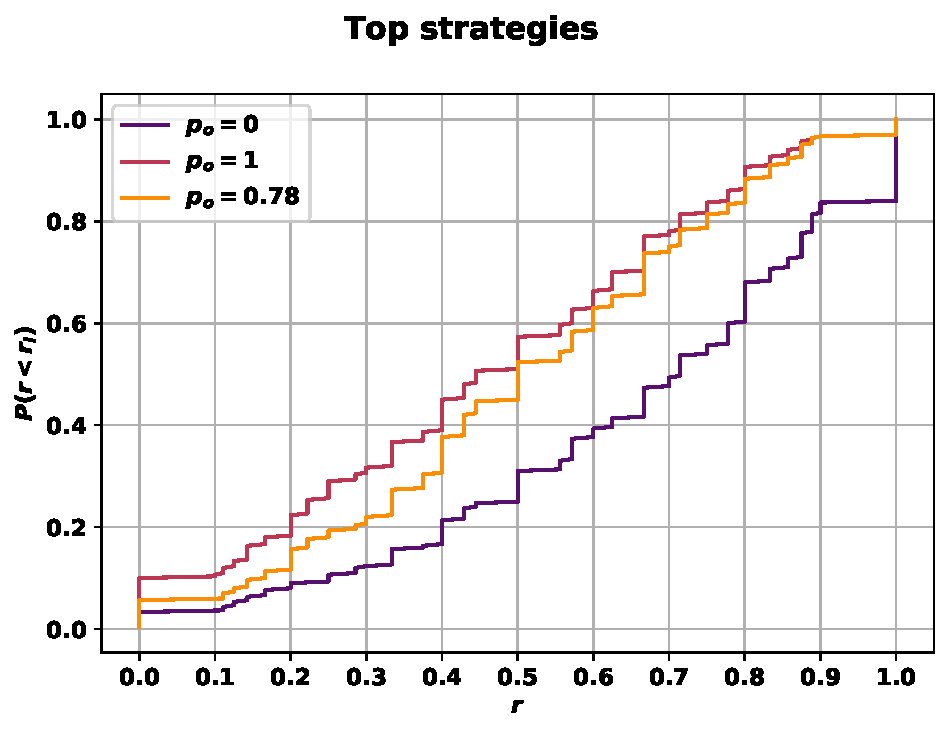
\includegraphics[width=\textwidth]{src/chapters/07/img/cfd_to_sequence_top_strategies.pdf}
    \end{subfigure}
    \begin{subfigure}{.45\textwidth}
    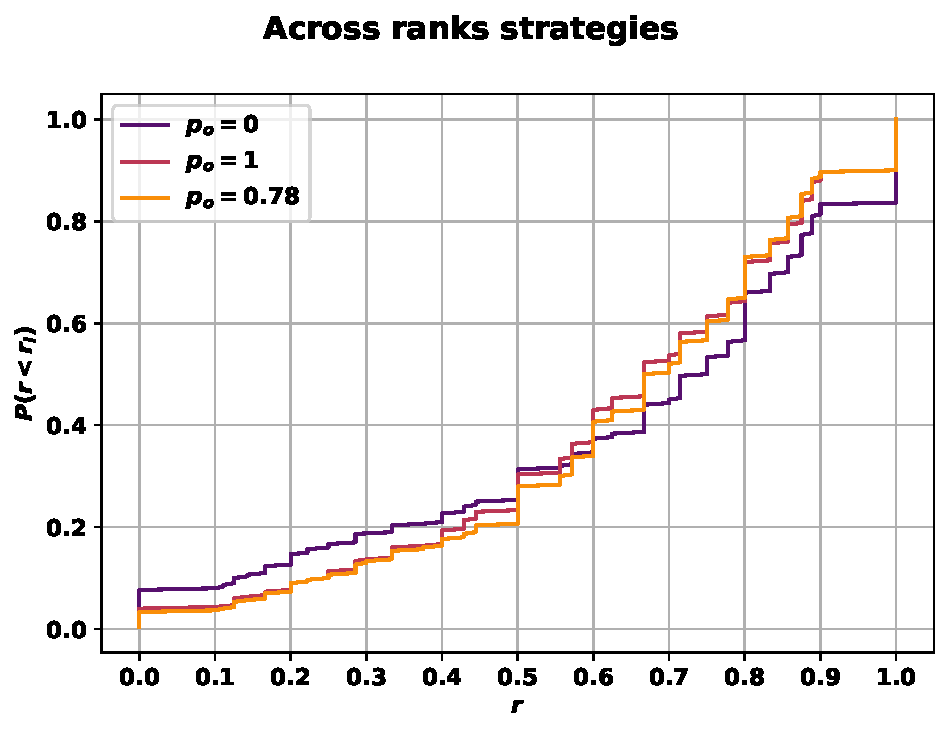
\includegraphics[width=\textwidth]{src/chapters/07/img/cfd_to_sequence_across_ranks_strategies.pdf}
    \end{subfigure}\hfill
    \begin{subfigure}{.45\textwidth}
    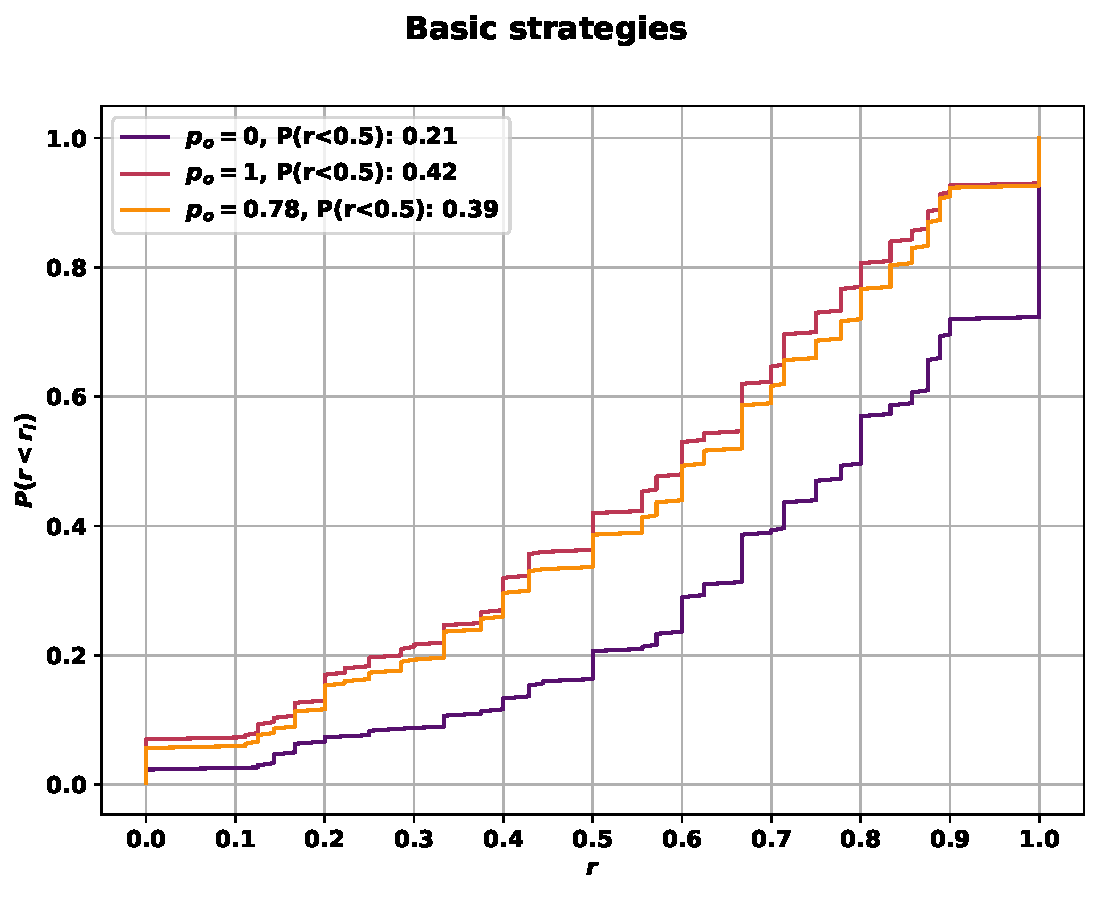
\includegraphics[width=\textwidth]{src/chapters/07/img/cfd_to_sequence_basic_strategies.pdf}
    \end{subfigure}
    \caption{The cumulative distribution function (CFD)
    for the \(r\) distributions for the LSTM strategies based on the StoS
    network.}\label{fig:cfd_s_to_s}
\end{figure}

\begin{figure}[!htbp]
    \begin{subfigure}{.45\textwidth}
    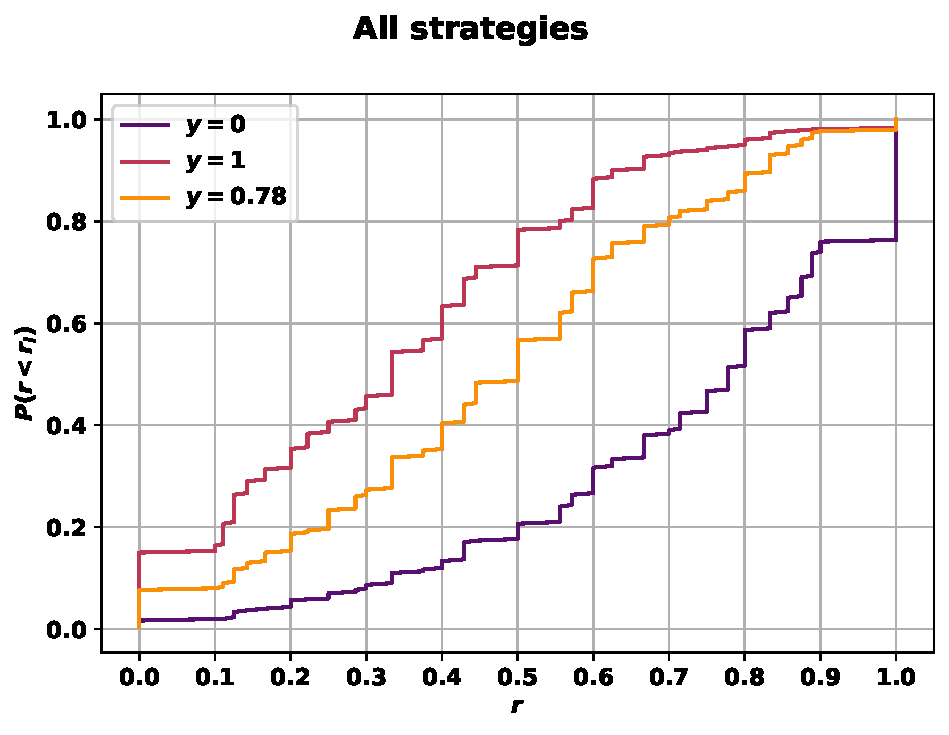
\includegraphics[width=\textwidth]{src/chapters/07/img/cfd_to_probability_all_strategies.pdf}
    \end{subfigure}\hfill
    \begin{subfigure}{.45\textwidth}
    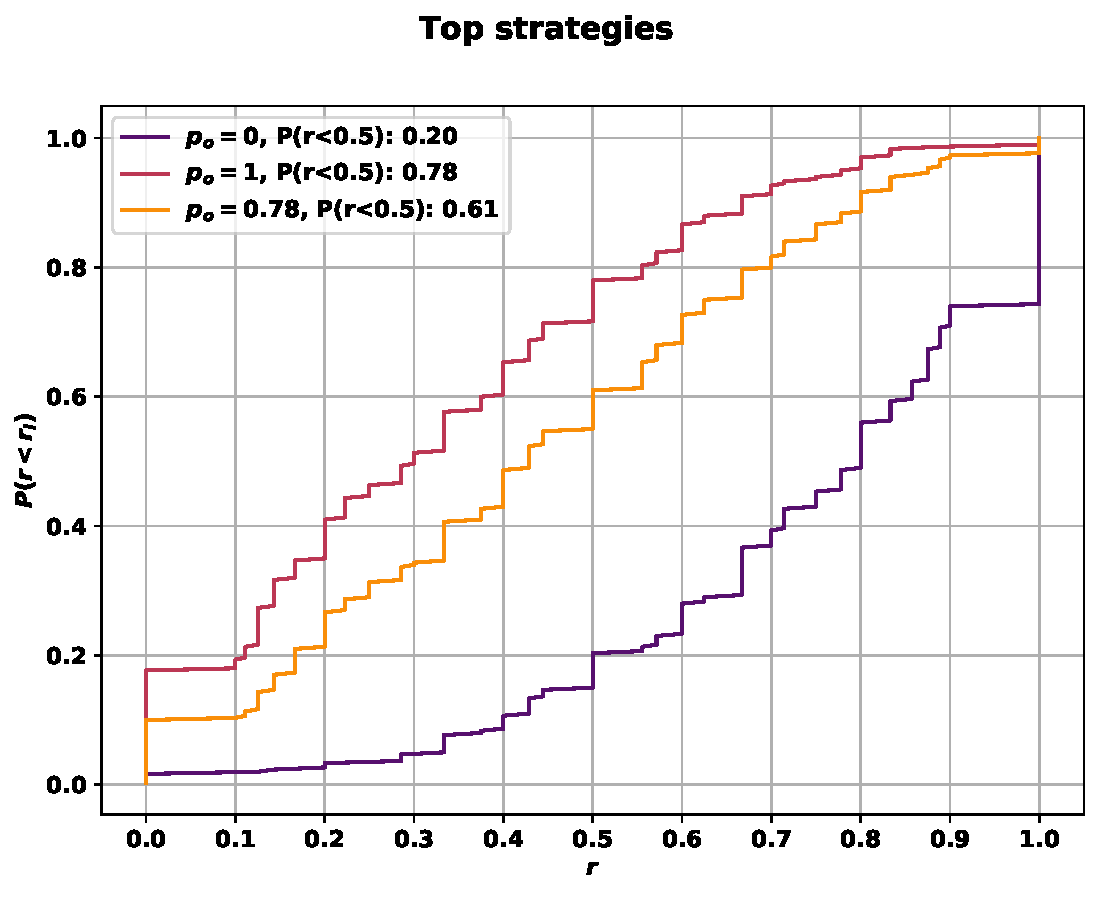
\includegraphics[width=\textwidth]{src/chapters/07/img/cfd_to_probability_top_strategies.pdf}
    \end{subfigure}
    \begin{subfigure}{.45\textwidth}
    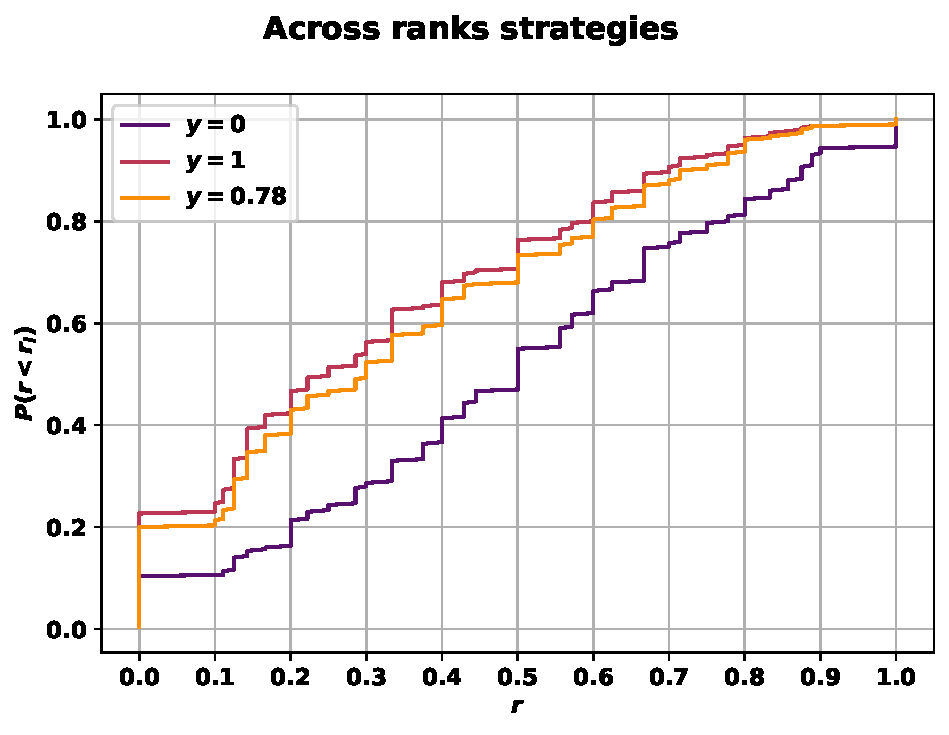
\includegraphics[width=\textwidth]{src/chapters/07/img/cfd_to_probability_across_ranks_strategies.pdf}
    \end{subfigure}\hfill
    \begin{subfigure}{.45\textwidth}
    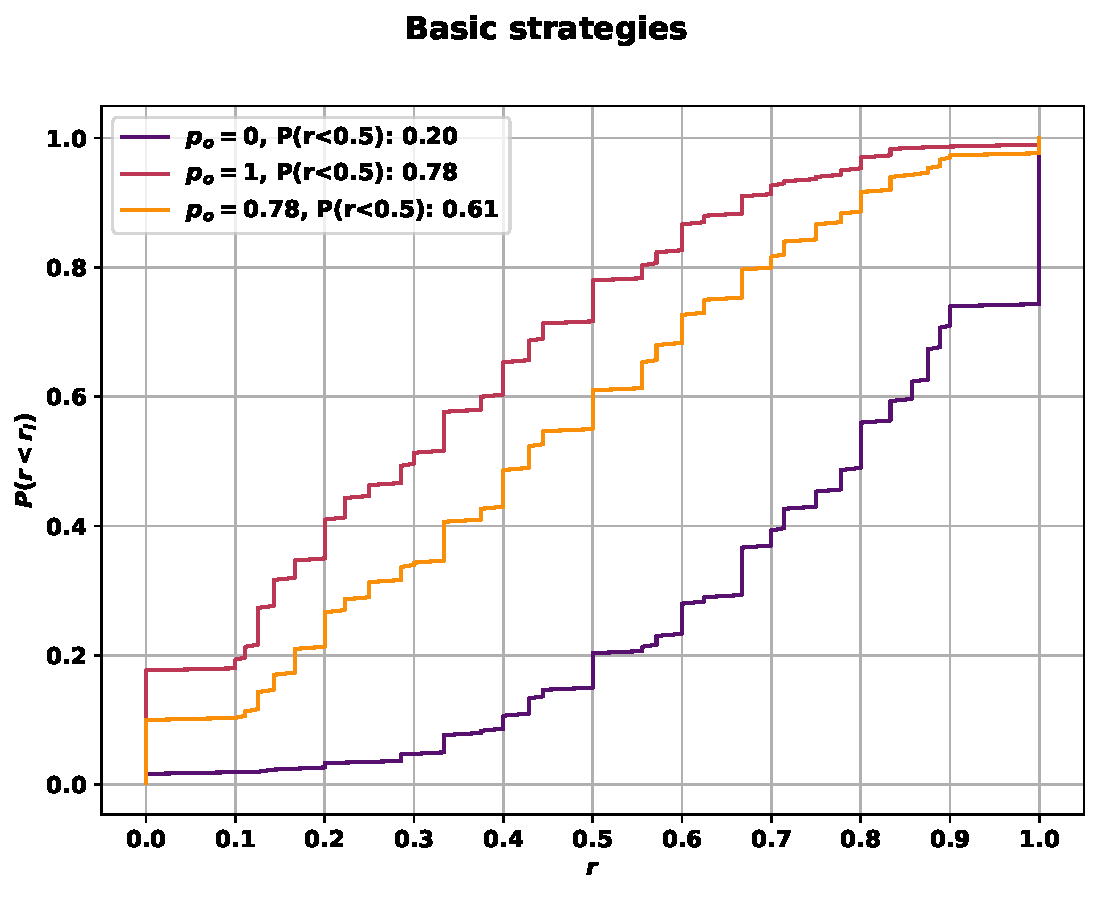
\includegraphics[width=\textwidth]{src/chapters/07/img/cfd_to_probability_basic_strategies.pdf}
    \end{subfigure}
    \caption{The cumulative distribution function (CFD)
    for the \(r\) distributions for the LSTM strategies based on the StoP
    network.}\label{fig:cfd_s_to_p}
\end{figure}

This section has evaluated the performance of \lstmstrategies newly introduced
IPD strategies based on LSTM networks. The performance of the strategies was
evaluated based on their normalised ranks in \metatournamentslstm standard
computer tournaments.

A total of 6 strategies have achieved a \(\bar{r}\) lower than 0.35. Thus, these
strategies have on average ranked on the top 30\% of a standard tournament.
These strategies have a 0.70-0.80 probability of ranking in top half of a
standard tournament. Overall the most successful strategies of the analysis have
been strategies that open with a cooperation.

Finally, the LSTM strategies that have been trained against the top ranked
strategies performed poorly. The top ranked strategies consisted of many trained
strategies from~\cite{Harper2017}. In~\cite{Harper2017} it was shown that these
strategies managed to exploit weak opponents whilst achieving mutual cooperation
with strong opponents. The best response sequences of these strategies could
have potentially only captured a single behaviour of these strategies, thus not
providing enough diverse training samples. This could have in turn made the LSTM
strategies less adaptable to diverse environments.

On the whole, the analysis of this section has shown that
the LSTM strategies
which were trained on the entire data set of best responses were successful
strategies regardless of the LSTM architecture. Both the StoS and StoP networks
have produced strategies that can win IPD tournaments, and on average rank on
the top 30\% of any given standard tournament. Moreover, the LSTM strategies
trained on subsets of the training data set, perform better when trained with
the StoP network than the StoS network. The StoP networks for the subsets have
been trained for a longer number of epochs compared to the StoP network over the
entire data set. An interesting question is whether the StoP strategy, trained
on the entire data set, would perform even better than it's equivalent StoS
strategy if it was trained for longer.

Having successfully trained high performing strategies using LSTM networks, 
the next section will attempt to qualify their behaviour.
\subsection{Fingerprinting the LSTM based strategies}

The 24 strategies that have been introduced in this Chapter are based on an LSTM
archetype. These strategies are based on a complex structure and interpreting
their behaviour is not trivial. The difference between the strategies is not
straightforward either. In Chapter~\ref{chapter:literature_review} a method that
produces a functional signature of a strategy called fingerprinting was
presented. More specifically, two types of fingerprints were discussed which
were the Ashlock fingerprints and the transitive fingerprints.

Ashlock's fingerprints~\cite{Ashlock2005, Ashlock2008, Ashlock2009,
Ashlock2010, Ashlock2006a} compute the score of a strategy against a spectrum of
opponents. The basic method is to play the strategy against a probe strategy
with varying noise parameters. The fingerprints for the \lstmstrategies
strategies based on Ashlock's approach have been generated for the probe
strategies Tit For Tat and Pavlov. These are given by
Figures~\ref{fig:ashlock_fingerprints_tft_s_to_s} -
\ref{fig:ashlock_fingerprints_pavlov_s_to_p}. Note that the strategies that
appear on the same row are of the same network type and have been trained on
the same training data set.

For Figures~\ref{fig:ashlock_fingerprints_tft_s_to_s} and
\ref{fig:ashlock_fingerprints_tft_s_to_p} Tit For Tat was used as the probe
strategy. It is demonstrated that the strategies on same row have similar fingerprints,
even though their opening move is different. The strategies however based on
different networks, or even different training data sets, exhibit different
behaviours. The only set of strategies that have similarities, regardless their
network architecture, is the strategies trained against the top performing
strategies.

\begin{figure}[!htbp]
    \begin{subfigure}{\textwidth}
        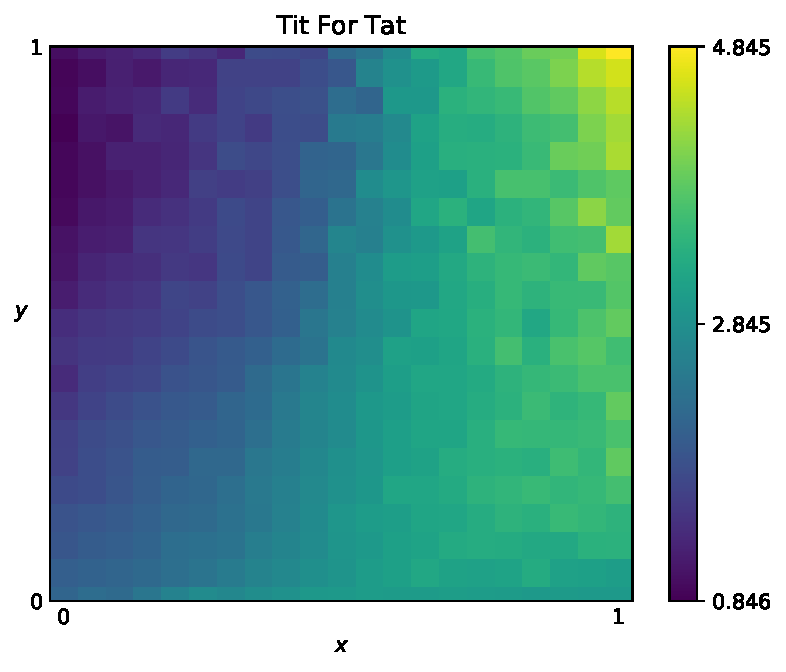
\includegraphics[width=.3\textwidth]{src/chapters/07/img/tit_for_tat_lstm_sequence_0.pdf}
        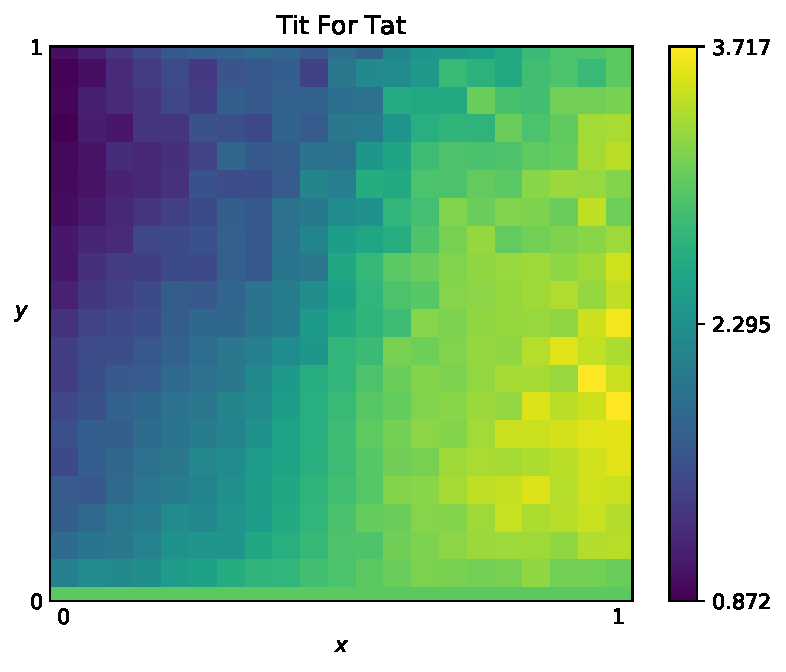
\includegraphics[width=.3\textwidth]{src/chapters/07/img/tit_for_tat_lstm_sequence_1.pdf}
        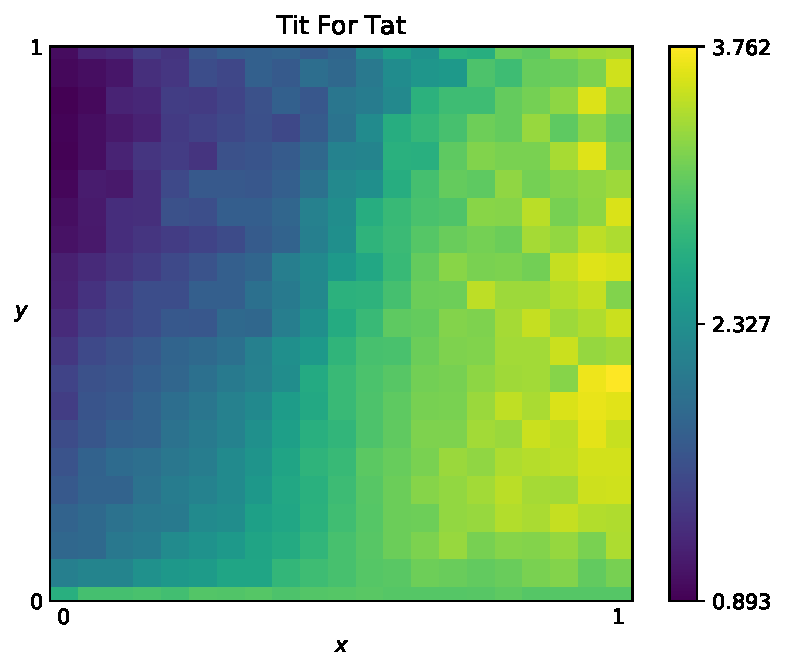
\includegraphics[width=.3\textwidth]{src/chapters/07/img/tit_for_tat_lstm_sequence_0_78.pdf}
        \caption{Strategies trained on the entire training data set.}
    \end{subfigure}
    \begin{subfigure}{\textwidth}
        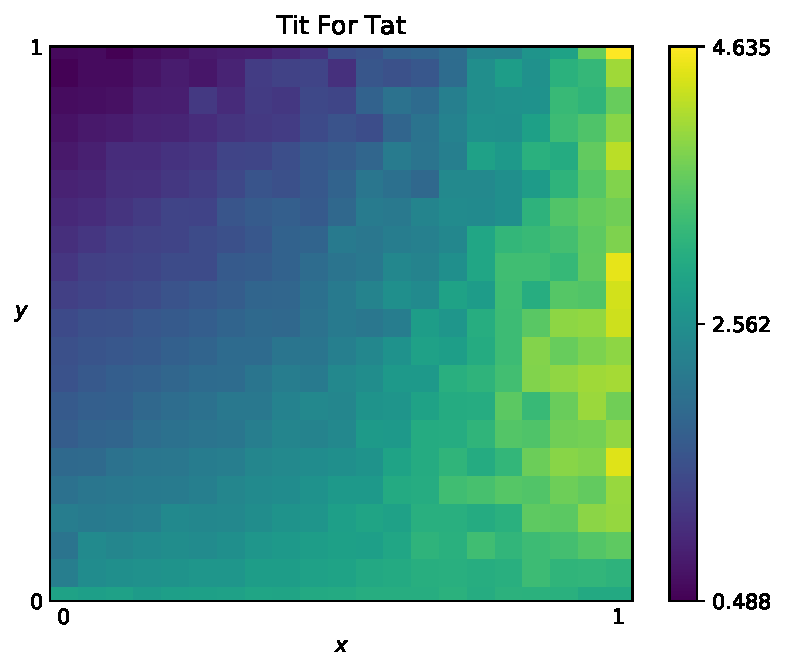
\includegraphics[width=.3\textwidth]{src/chapters/07/img/tit_for_tat_top_twenty_sequence_0.pdf}
        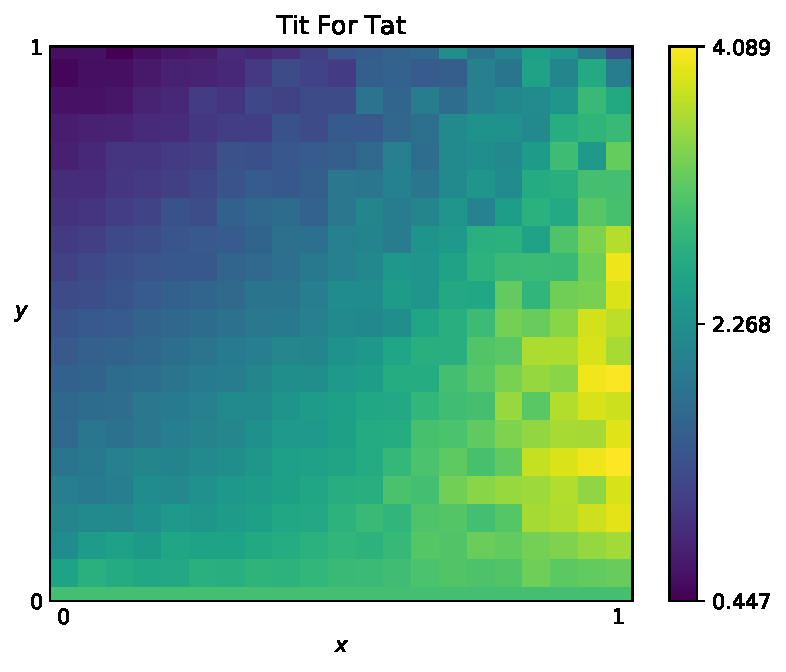
\includegraphics[width=.3\textwidth]{src/chapters/07/img/tit_for_tat_top_twenty_sequence_1.pdf}
        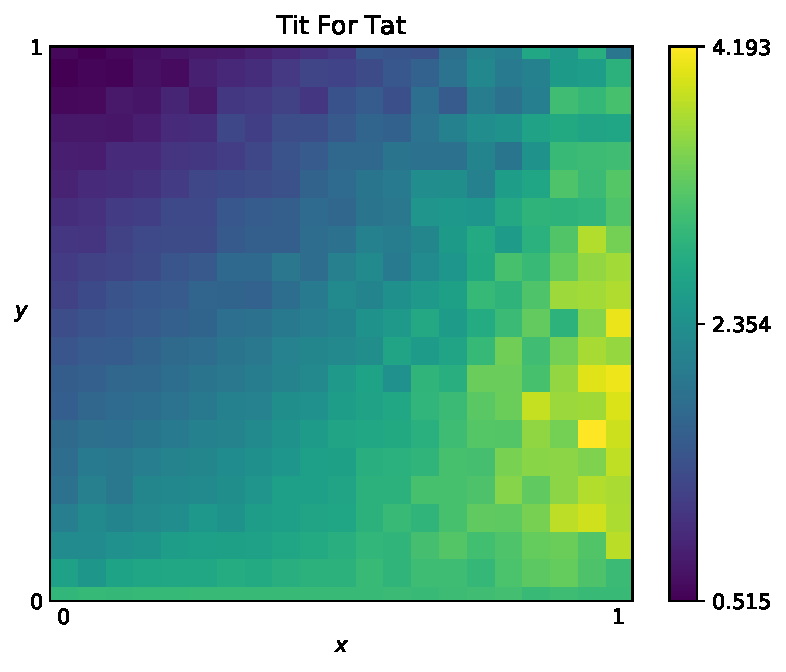
\includegraphics[width=.3\textwidth]{src/chapters/07/img/tit_for_tat_top_twenty_sequence_0_78.pdf}
        \caption{Strategies trained against the top performing strategies.}
    \end{subfigure}
    \begin{subfigure}{\textwidth}
        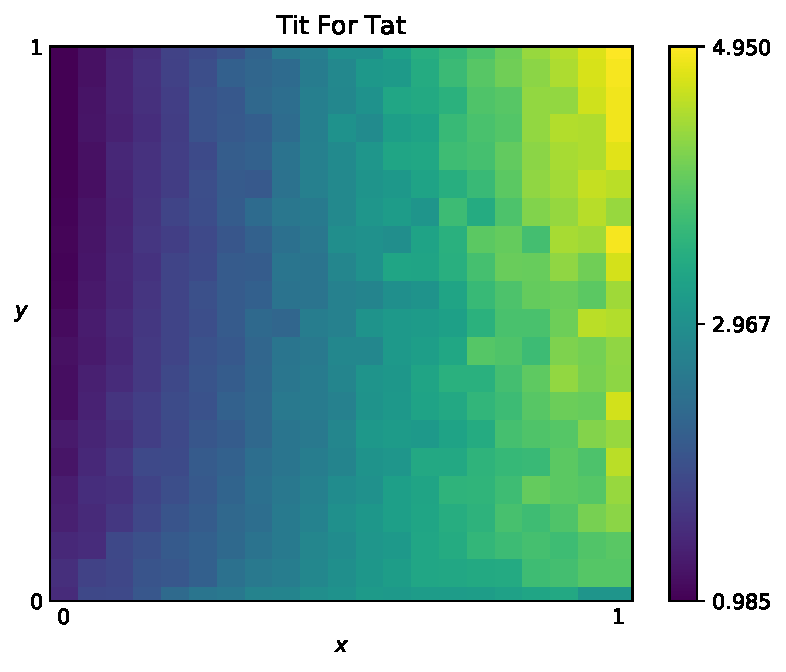
\includegraphics[width=.3\textwidth]{src/chapters/07/img/tit_for_tat_twenty_sequence_0.pdf}
        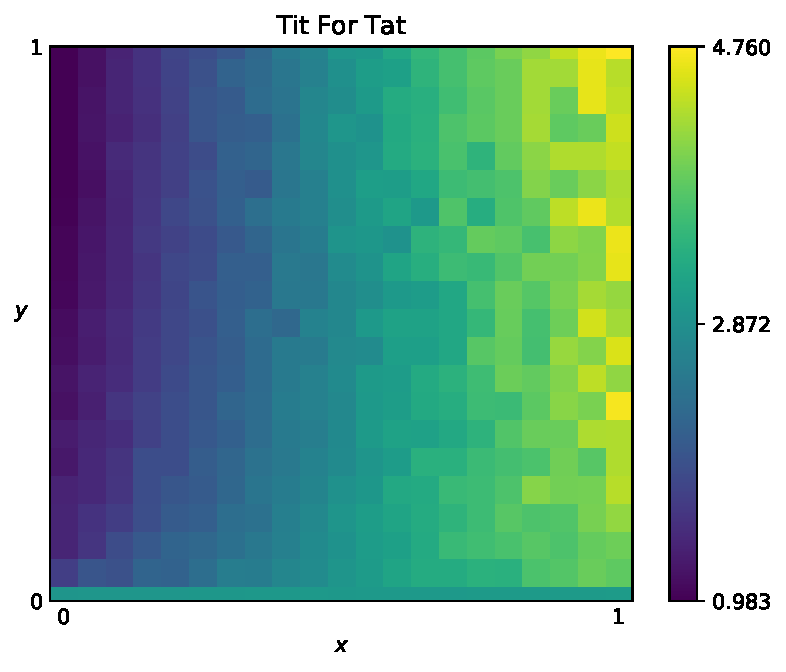
\includegraphics[width=.3\textwidth]{src/chapters/07/img/tit_for_tat_twenty_sequence_1.pdf}
        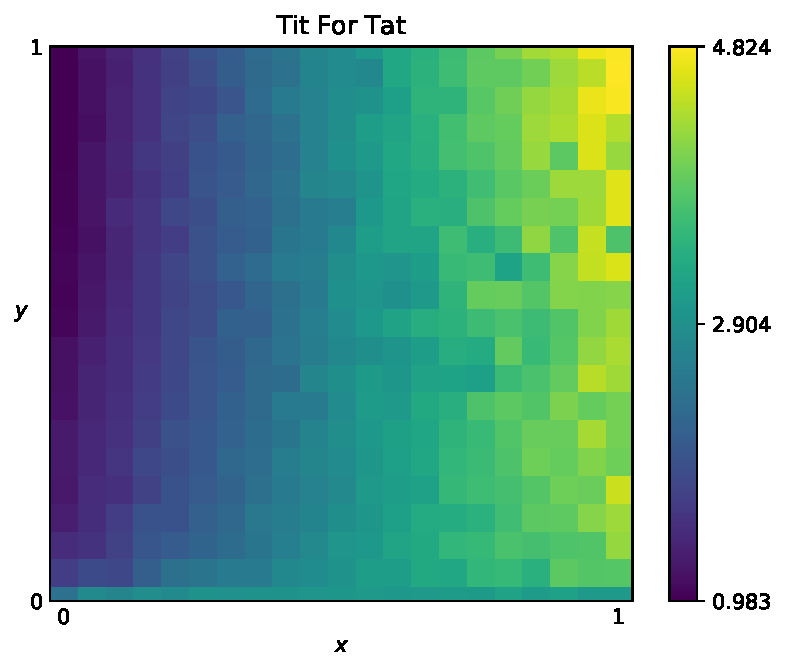
\includegraphics[width=.3\textwidth]{src/chapters/07/img/tit_for_tat_twenty_sequence_0_78.pdf}
        \caption{Strategies trained against the across the ranks strategies.}
    \end{subfigure}
    \begin{subfigure}{\textwidth}
        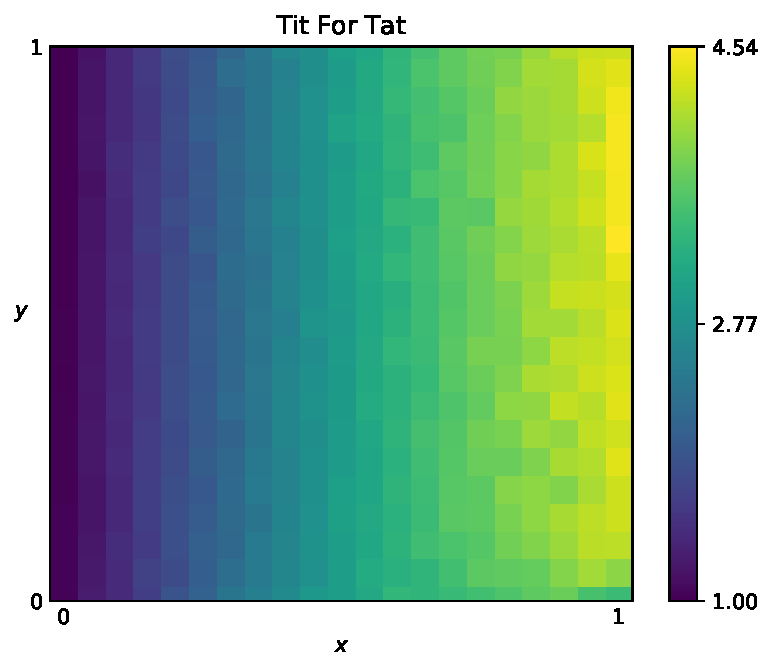
\includegraphics[width=.3\textwidth]{src/chapters/07/img/tit_for_tat_basic_sequence_0.pdf}
        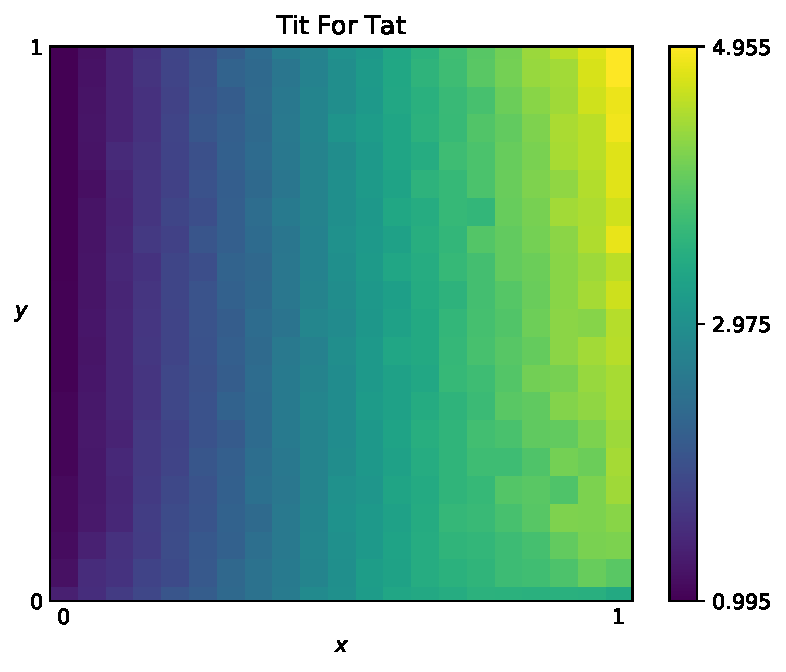
\includegraphics[width=.3\textwidth]{src/chapters/07/img/tit_for_tat_basic_sequence_1.pdf}
        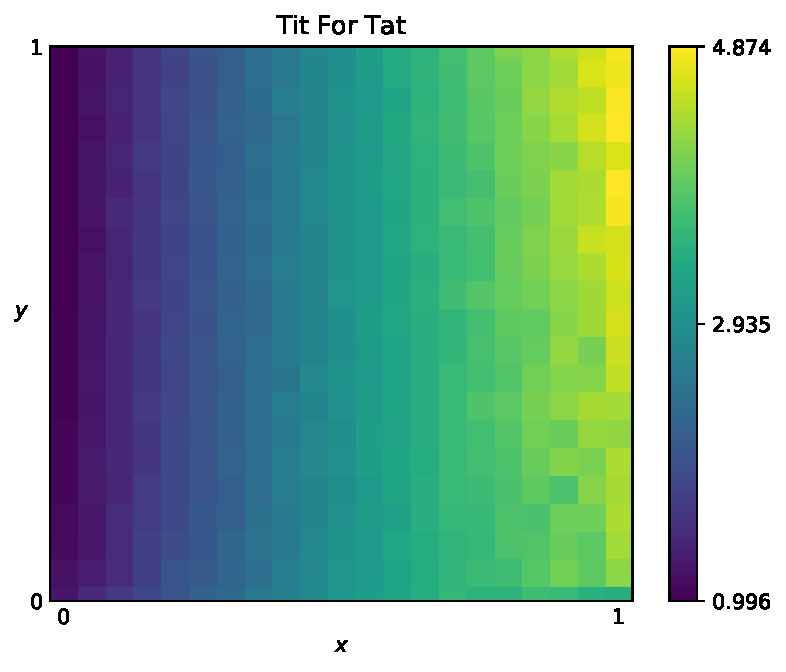
\includegraphics[width=.3\textwidth]{src/chapters/07/img/tit_for_tat_basic_sequence_0_78.pdf}
        \caption{Strategies trained against basic strategies.}
    \end{subfigure}
    \caption{Ashlock's fingerprints for the LSTM strategies based on the StoS
    network when Tit For Tat is the probe strategy.}\label{fig:ashlock_fingerprints_tft_s_to_s}
\end{figure}

\begin{figure}[!htbp]
    \begin{subfigure}{\textwidth}
        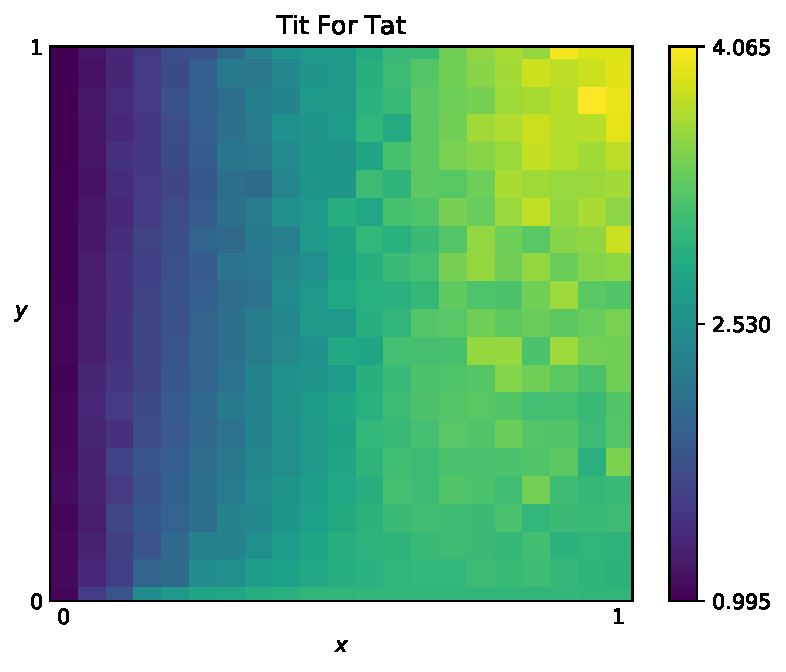
\includegraphics[width=.3\textwidth]{src/chapters/07/img/tit_for_tat_lstm_classification_0.pdf}
        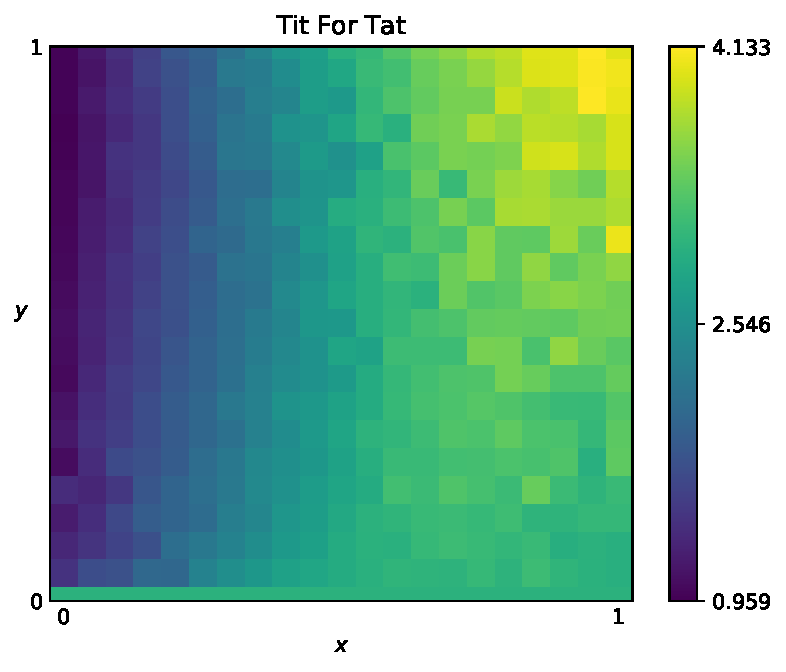
\includegraphics[width=.3\textwidth]{src/chapters/07/img/tit_for_tat_lstm_classification_1.pdf}
        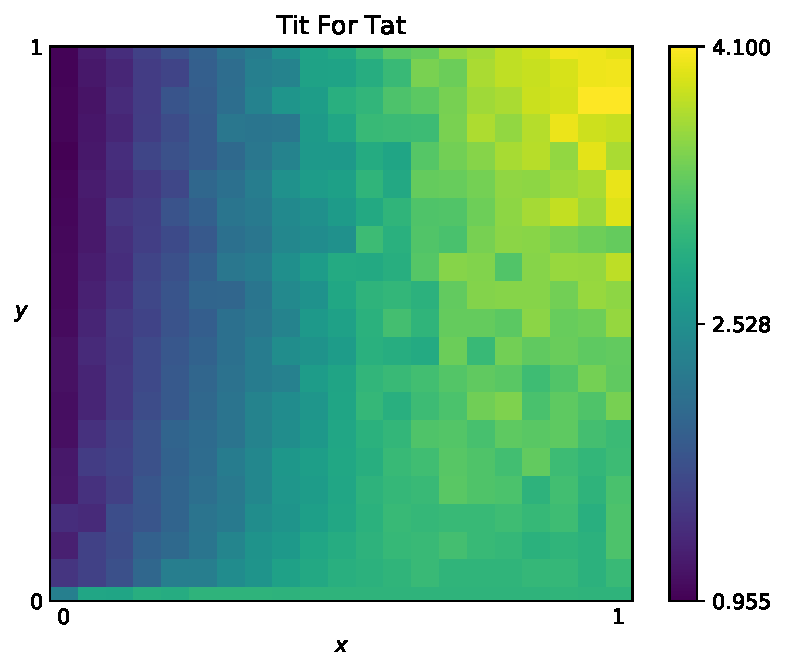
\includegraphics[width=.3\textwidth]{src/chapters/07/img/tit_for_tat_lstm_classification_0_78.pdf}
        \caption{Strategies trained on the entire training data set.}
    \end{subfigure}
    \begin{subfigure}{\textwidth}
        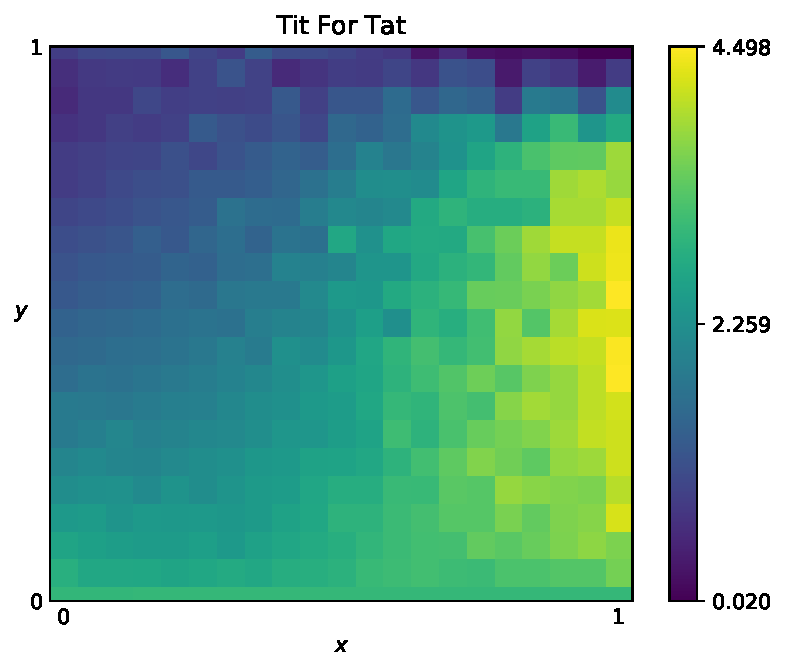
\includegraphics[width=.3\textwidth]{src/chapters/07/img/tit_for_tat_top_twenty_classification_0.pdf}
        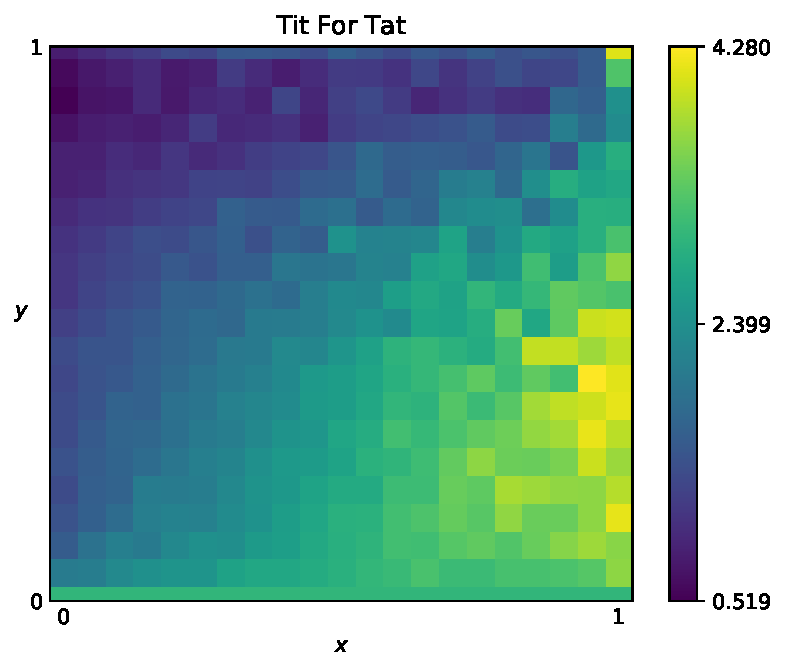
\includegraphics[width=.3\textwidth]{src/chapters/07/img/tit_for_tat_top_twenty_classification_1.pdf}
        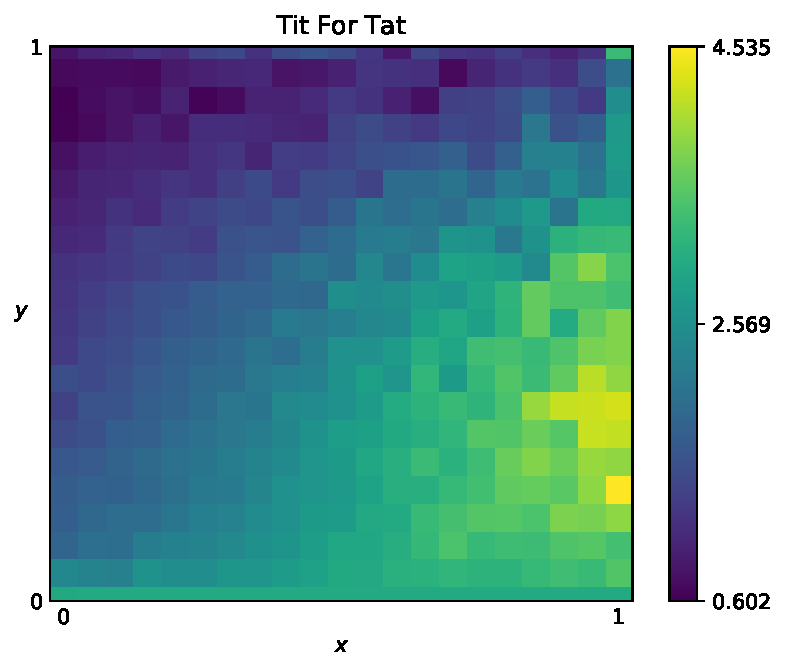
\includegraphics[width=.3\textwidth]{src/chapters/07/img/tit_for_tat_top_twenty_classification_0_78.pdf}
        \caption{Strategies trained against the top performing strategies.}
    \end{subfigure}
    \begin{subfigure}{\textwidth}
        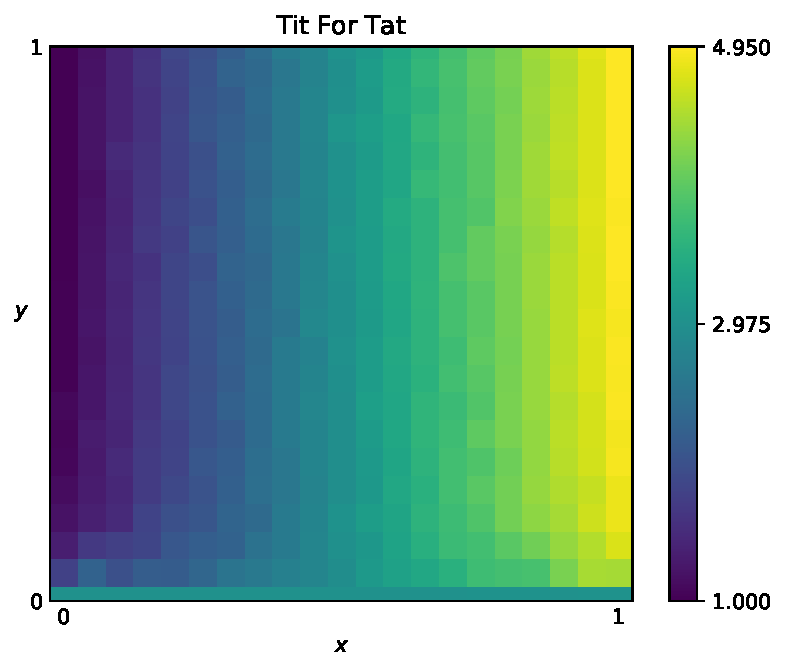
\includegraphics[width=.3\textwidth]{src/chapters/07/img/tit_for_tat_twenty_classification_0.pdf}
        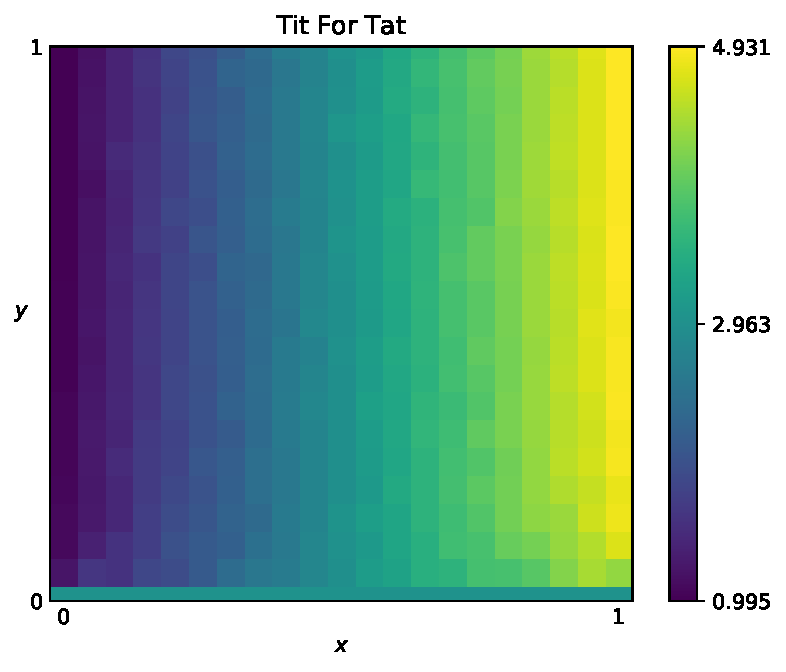
\includegraphics[width=.3\textwidth]{src/chapters/07/img/tit_for_tat_twenty_classification_1.pdf}
        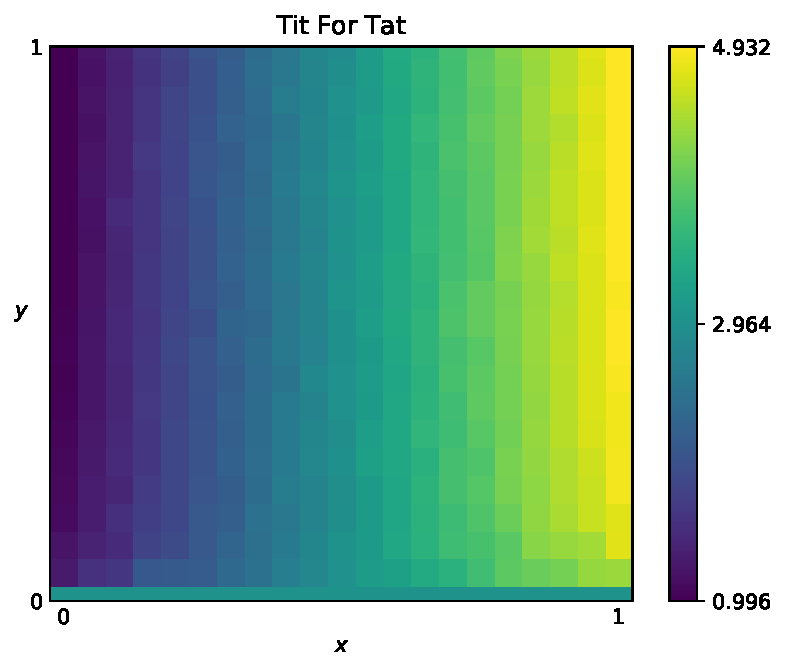
\includegraphics[width=.3\textwidth]{src/chapters/07/img/tit_for_tat_twenty_classification_0_78.pdf}
        \caption{Strategies trained against the across the ranks strategies.}
    \end{subfigure}
    \begin{subfigure}{\textwidth}
        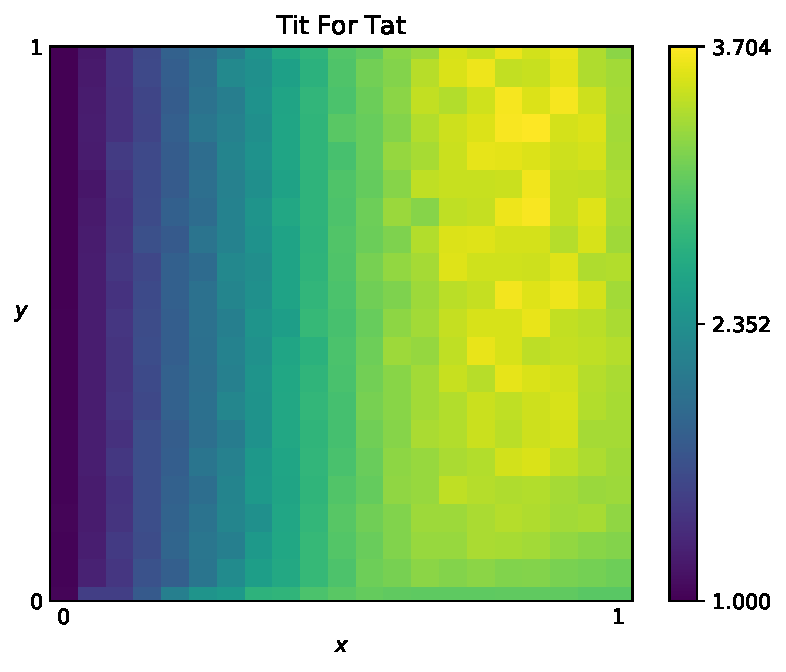
\includegraphics[width=.3\textwidth]{src/chapters/07/img/tit_for_tat_basic_classification_0.pdf}
        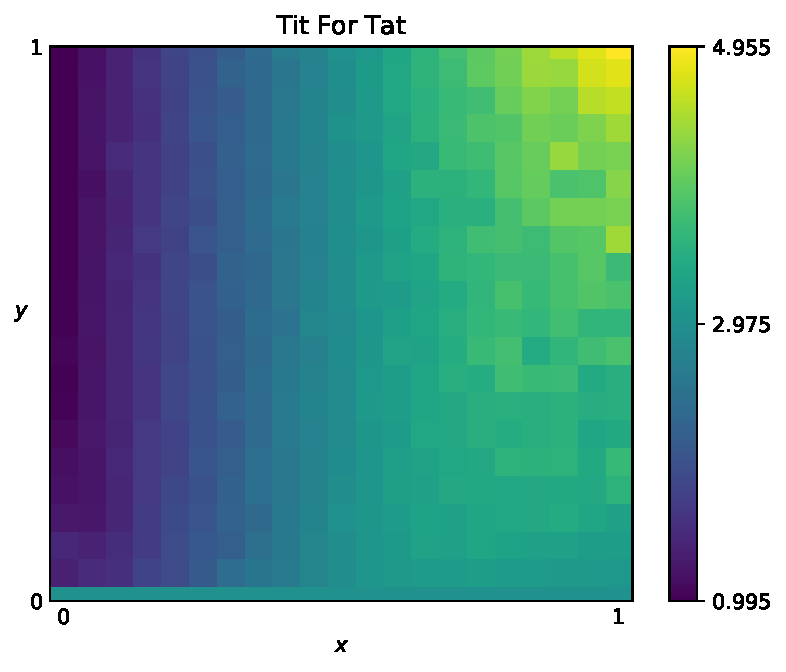
\includegraphics[width=.3\textwidth]{src/chapters/07/img/tit_for_tat_basic_classification_1.pdf}
        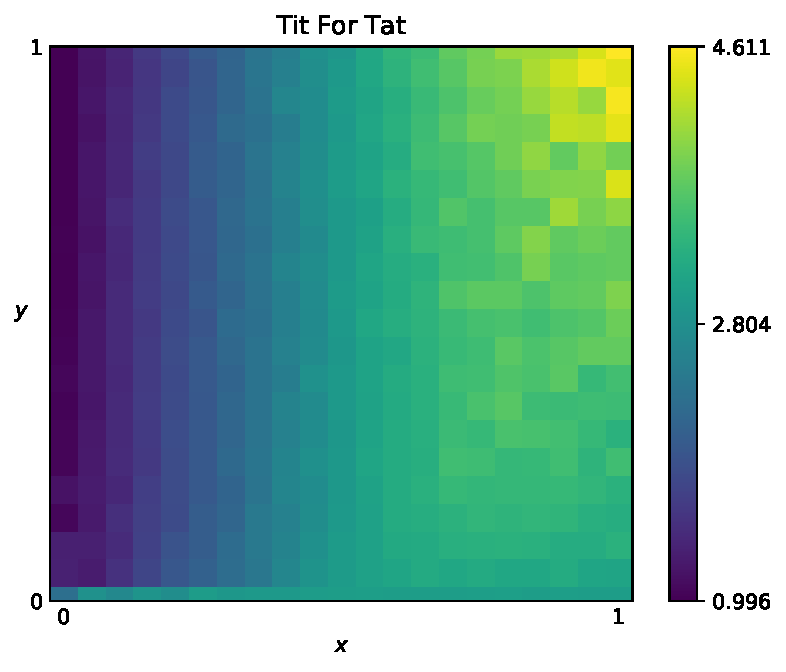
\includegraphics[width=.3\textwidth]{src/chapters/07/img/tit_for_tat_basic_classification_0_78.pdf}
        \caption{Strategies trained against basic strategies.}
    \end{subfigure}
    \caption{Ashlock's fingerprints for the LSTM strategies based on the StoP
    network when Tit For Tat is the probe strategy.}\label{fig:ashlock_fingerprints_tft_s_to_p}
\end{figure}

Figures \ref{fig:ashlock_fingerprints_pavlov_s_to_s} and
\ref{fig:ashlock_fingerprints_pavlov_s_to_p} give the Ashlock fingerprints
whilst Pavlov is used as a probe. These fingerprints, across the network types,
training data set and opening moves appear to be more similar. 

\begin{figure}[!htbp]
    \begin{subfigure}{\textwidth}
        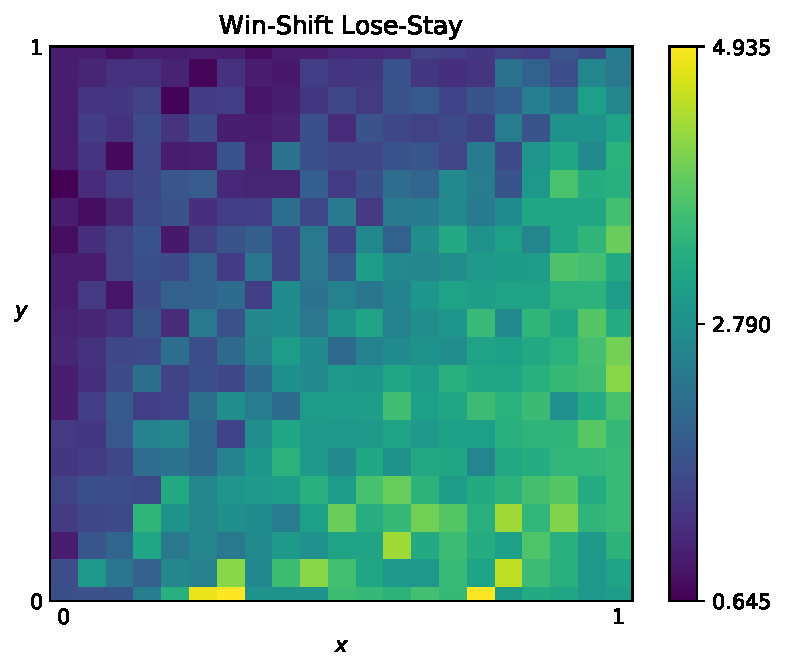
\includegraphics[width=.3\textwidth]{src/chapters/07/img/win_shift_lose_stay_lstm_sequence_0.pdf}
        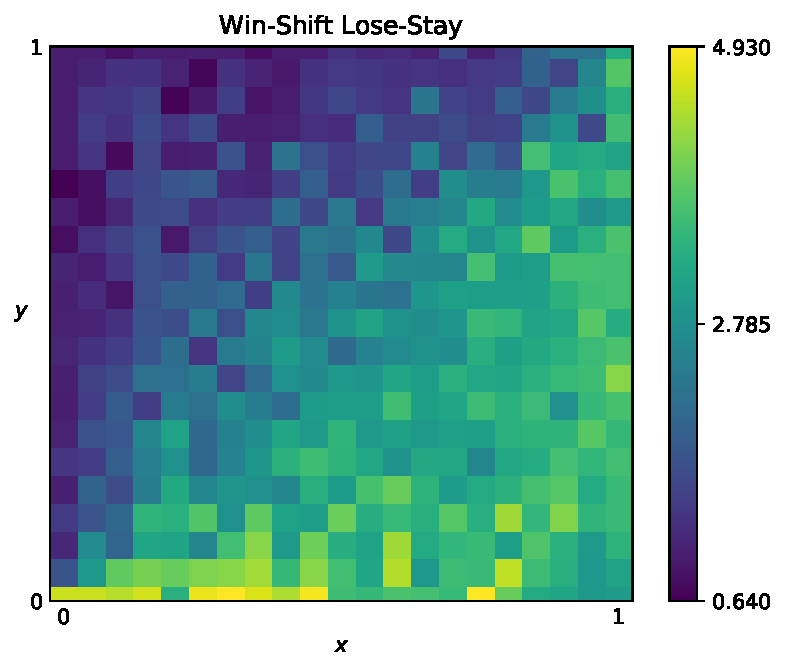
\includegraphics[width=.3\textwidth]{src/chapters/07/img/win_shift_lose_stay_lstm_sequence_1.pdf}
        \includegraphics[width=.3\textwidth]{src/chapters/07/img/win_shift_lose_stay_lstm_sequence_0_78.pdf}
        \caption{Strategies trained on the entire training data set.}
    \end{subfigure}
    \begin{subfigure}{\textwidth}
        \includegraphics[width=.3\textwidth]{src/chapters/07/img/win_shift_lose_stay_top_twenty_sequence_0.pdf}
        \includegraphics[width=.3\textwidth]{src/chapters/07/img/win_shift_lose_stay_top_twenty_sequence_1.pdf}
        \includegraphics[width=.3\textwidth]{src/chapters/07/img/win_shift_lose_stay_top_twenty_sequence_0_78.pdf}
        \caption{Strategies trained against the top performing strategies.}
    \end{subfigure}
    \begin{subfigure}{\textwidth}
        \includegraphics[width=.3\textwidth]{src/chapters/07/img/win_shift_lose_stay_twenty_sequence_0.pdf}
        \includegraphics[width=.3\textwidth]{src/chapters/07/img/win_shift_lose_stay_twenty_sequence_1.pdf}
        \includegraphics[width=.3\textwidth]{src/chapters/07/img/win_shift_lose_stay_twenty_sequence_0_78.pdf}
        \caption{Strategies trained against the across the ranks strategies.}
    \end{subfigure}
    \begin{subfigure}{\textwidth}
        \includegraphics[width=.3\textwidth]{src/chapters/07/img/win_shift_lose_stay_basic_sequence_0.pdf}
        \includegraphics[width=.3\textwidth]{src/chapters/07/img/win_shift_lose_stay_basic_sequence_1.pdf}
        \includegraphics[width=.3\textwidth]{src/chapters/07/img/win_shift_lose_stay_basic_sequence_0_78.pdf}
        \caption{Strategies trained against basic strategies.}
    \end{subfigure}
    \caption{Ashlock's fingerprints for the LSTM strategies based on the StoS
    network when Pavlov is the probe strategy.}\label{fig:ashlock_fingerprints_pavlov_s_to_s}
\end{figure}

\begin{figure}[!htbp]
    \begin{subfigure}{\textwidth}
        \includegraphics[width=.3\textwidth]{src/chapters/07/img/win_shift_lose_stay_lstm_classification_0.pdf}
        \includegraphics[width=.3\textwidth]{src/chapters/07/img/win_shift_lose_stay_lstm_classification_1.pdf}
        \includegraphics[width=.3\textwidth]{src/chapters/07/img/win_shift_lose_stay_lstm_classification_0_78.pdf}
        \caption{Strategies trained on the entire training data set.}
    \end{subfigure}
    \begin{subfigure}{\textwidth}
        \includegraphics[width=.3\textwidth]{src/chapters/07/img/win_shift_lose_stay_top_twenty_classification_0.pdf}
        \includegraphics[width=.3\textwidth]{src/chapters/07/img/win_shift_lose_stay_top_twenty_classification_1.pdf}
        \includegraphics[width=.3\textwidth]{src/chapters/07/img/win_shift_lose_stay_top_twenty_classification_0_78.pdf}
        \caption{Strategies trained against the top performing strategies.}
    \end{subfigure}
    \begin{subfigure}{\textwidth}
        \includegraphics[width=.3\textwidth]{src/chapters/07/img/win_shift_lose_stay_twenty_classification_0.pdf}
        \includegraphics[width=.3\textwidth]{src/chapters/07/img/win_shift_lose_stay_twenty_classification_1.pdf}
        \includegraphics[width=.3\textwidth]{src/chapters/07/img/win_shift_lose_stay_twenty_classification_0_78.pdf}
        \caption{Strategies trained against the across the ranks strategies.}
    \end{subfigure}
    \begin{subfigure}{\textwidth}
        \includegraphics[width=.3\textwidth]{src/chapters/07/img/win_shift_lose_stay_basic_classification_0.pdf}
        \includegraphics[width=.3\textwidth]{src/chapters/07/img/win_shift_lose_stay_basic_classification_1.pdf}
        \includegraphics[width=.3\textwidth]{src/chapters/07/img/win_shift_lose_stay_basic_classification_0_78.pdf}
        \caption{Strategies trained against basic strategies.}
    \end{subfigure}
    \caption{Ashlock's fingerprints for the LSTM strategies based on the StoP
    network when Pavlov is the probe strategy.}\label{fig:ashlock_fingerprints_pavlov_s_to_p}
\end{figure}

Ashlock fingerprints do not give an immediate qualifiable understanding of behaviour and so
to further explore the similarities of the strategies a set of more
interpretable fingerprints, the transitive fingerprints implemented in APL, have
also been generated. The transitive fingerprints represent the cooperation rate
of a strategy against a set of opponents over a number of turns. There are two
set of opponents used here to generate the transitive fingerprints. These are
the collection of strategies from~\cite{Stewart2012} and
from~\cite{Beaufils1997}. The transitive fingerprints are given by
Figures~\ref{fig:transitive_fingerprints_stewart_s_to_s}
-\ref{fig:transitive_fingerprints_beautil_s_to_p}.

The differences between the strategies are more distinct using the transitive
fingerprinting method. It can be seen that the LSTM strategies do indeed behave
differently against the same list of opponents.

Furthermore, two more observations can be made by the transitive fingerprints.
Initially, that the strategies that open with cooperation achieve a higher
cooperation rate compared to the strategies (on the same row) that do not.
Secondly, the LSTM strategies appear to use the opening turns to decide on a play.
This is demonstrated but the fact that there is some variation in the opening
moves of each fingerprint, but following the opening turns the patterns became
more stable.

\begin{figure}[!htbp]
    \begin{subfigure}{\textwidth}
        \includegraphics[width=.3\textwidth]{src/chapters/07/img/stewart_lstm_sequence_0.pdf}
        \includegraphics[width=.3\textwidth]{src/chapters/07/img/stewart_lstm_sequence_1.pdf}
        \includegraphics[width=.3\textwidth]{src/chapters/07/img/stewart_lstm_sequence_0_78.pdf}
        \caption{Strategies trained on the entire training data set.}
    \end{subfigure}
    \begin{subfigure}{\textwidth}
        \includegraphics[width=.3\textwidth]{src/chapters/07/img/stewart_top_twenty_sequence_0.pdf}
        \includegraphics[width=.3\textwidth]{src/chapters/07/img/stewart_top_twenty_sequence_1.pdf}
        \includegraphics[width=.3\textwidth]{src/chapters/07/img/stewart_top_twenty_sequence_0_78.pdf}
        \caption{Strategies trained against the top performing strategies.}
    \end{subfigure}
    \begin{subfigure}{\textwidth}
        \includegraphics[width=.3\textwidth]{src/chapters/07/img/stewart_twenty_sequence_0.pdf}
        \includegraphics[width=.3\textwidth]{src/chapters/07/img/stewart_twenty_sequence_1.pdf}
        \includegraphics[width=.3\textwidth]{src/chapters/07/img/stewart_twenty_sequence_0_78.pdf}
        \caption{Strategies trained against the across the ranks strategies.}
    \end{subfigure}
    \begin{subfigure}{\textwidth}
        \includegraphics[width=.3\textwidth]{src/chapters/07/img/stewart_basic_sequence_0.pdf}
        \includegraphics[width=.3\textwidth]{src/chapters/07/img/stewart_basic_sequence_1.pdf}
        \includegraphics[width=.3\textwidth]{src/chapters/07/img/stewart_basic_sequence_0_78.pdf}
        \caption{Strategies trained against basic strategies.}
    \end{subfigure}
    \caption{Transitive fingerprints for the LSTM strategies based on the StoS
    network against the list of opponents from~\cite{Stewart2012}.}\label{fig:transitive_fingerprints_stewart_s_to_s}
\end{figure}

\begin{figure}[!htbp]
    \begin{subfigure}{\textwidth}
        \includegraphics[width=.3\textwidth]{src/chapters/07/img/stewart_lstm_classification_0.pdf}
        \includegraphics[width=.3\textwidth]{src/chapters/07/img/stewart_lstm_classification_1.pdf}
        \includegraphics[width=.3\textwidth]{src/chapters/07/img/stewart_lstm_classification_0_78.pdf}
        \caption{Strategies trained on the entire training data set.}
    \end{subfigure}
    \begin{subfigure}{\textwidth}
        \includegraphics[width=.3\textwidth]{src/chapters/07/img/stewart_top_twenty_classification_0.pdf}
        \includegraphics[width=.3\textwidth]{src/chapters/07/img/stewart_top_twenty_classification_1.pdf}
        \includegraphics[width=.3\textwidth]{src/chapters/07/img/stewart_top_twenty_classification_0_78.pdf}
        \caption{Strategies trained against the top performing strategies.}
    \end{subfigure}
    \begin{subfigure}{\textwidth}
        \includegraphics[width=.3\textwidth]{src/chapters/07/img/stewart_twenty_classification_0.pdf}
        \includegraphics[width=.3\textwidth]{src/chapters/07/img/stewart_twenty_classification_1.pdf}
        \includegraphics[width=.3\textwidth]{src/chapters/07/img/stewart_twenty_classification_0_78.pdf}
        \caption{Strategies trained against the across the ranks strategies.}
    \end{subfigure}
    \begin{subfigure}{\textwidth}
        \includegraphics[width=.3\textwidth]{src/chapters/07/img/stewart_basic_classification_0.pdf}
        \includegraphics[width=.3\textwidth]{src/chapters/07/img/stewart_basic_classification_1.pdf}
        \includegraphics[width=.3\textwidth]{src/chapters/07/img/stewart_basic_classification_0_78.pdf}
        \caption{Strategies trained against basic strategies.}
    \end{subfigure}
    \caption{Transitive fingerprints for the LSTM strategies based on the StoP
    network against the list of opponents from~\cite{Stewart2012}.}\label{fig:transitive_fingerprints_stewart_s_to_p}
\end{figure}

\begin{figure}[!htbp]
    \begin{subfigure}{\textwidth}
        \includegraphics[width=.3\textwidth]{src/chapters/07/img/beautil_lstm_sequence_0.pdf}
        \includegraphics[width=.3\textwidth]{src/chapters/07/img/beautil_lstm_sequence_1.pdf}
        \includegraphics[width=.3\textwidth]{src/chapters/07/img/beautil_lstm_sequence_0_78.pdf}
        \caption{Strategies trained on the entire training data set.}
    \end{subfigure}
    \begin{subfigure}{\textwidth}
        \includegraphics[width=.3\textwidth]{src/chapters/07/img/beautil_top_twenty_sequence_0.pdf}
        \includegraphics[width=.3\textwidth]{src/chapters/07/img/beautil_top_twenty_sequence_1.pdf}
        \includegraphics[width=.3\textwidth]{src/chapters/07/img/beautil_top_twenty_sequence_0_78.pdf}
        \caption{Strategies trained against the top performing strategies.}
    \end{subfigure}
    \begin{subfigure}{\textwidth}
        \includegraphics[width=.3\textwidth]{src/chapters/07/img/beautil_twenty_sequence_0.pdf}
        \includegraphics[width=.3\textwidth]{src/chapters/07/img/beautil_twenty_sequence_1.pdf}
        \includegraphics[width=.3\textwidth]{src/chapters/07/img/beautil_twenty_sequence_0_78.pdf}
        \caption{Strategies trained against the across the ranks strategies.}
    \end{subfigure}
    \begin{subfigure}{\textwidth}
        \includegraphics[width=.3\textwidth]{src/chapters/07/img/beautil_basic_sequence_0.pdf}
        \includegraphics[width=.3\textwidth]{src/chapters/07/img/beautil_basic_sequence_1.pdf}
        \includegraphics[width=.3\textwidth]{src/chapters/07/img/beautil_basic_sequence_0_78.pdf}
        \caption{Strategies trained against basic strategies.}
    \end{subfigure}
    \caption{Transitive fingerprints for the LSTM strategies based on the StoS
    network against the list of opponents from~\cite{Beaufils1997}.}\label{fig:transitive_fingerprints_beautil_s_to_s}
\end{figure}

\begin{figure}[!htbp]
    \begin{subfigure}{\textwidth}
        \includegraphics[width=.3\textwidth]{src/chapters/07/img/beautil_lstm_classification_0.pdf}
        \includegraphics[width=.3\textwidth]{src/chapters/07/img/beautil_lstm_classification_1.pdf}
        \includegraphics[width=.3\textwidth]{src/chapters/07/img/beautil_lstm_classification_0_78.pdf}
        \caption{Strategies trained on the entire training data set.}
    \end{subfigure}
    \begin{subfigure}{\textwidth}
        \includegraphics[width=.3\textwidth]{src/chapters/07/img/beautil_top_twenty_classification_0.pdf}
        \includegraphics[width=.3\textwidth]{src/chapters/07/img/beautil_top_twenty_classification_1.pdf}
        \includegraphics[width=.3\textwidth]{src/chapters/07/img/beautil_top_twenty_classification_0_78.pdf}
        \caption{Strategies trained against the top performing strategies.}
    \end{subfigure}
    \begin{subfigure}{\textwidth}
        \includegraphics[width=.3\textwidth]{src/chapters/07/img/beautil_twenty_classification_0.pdf}
        \includegraphics[width=.3\textwidth]{src/chapters/07/img/beautil_twenty_classification_1.pdf}
        \includegraphics[width=.3\textwidth]{src/chapters/07/img/beautil_twenty_classification_0_78.pdf}
        \caption{Strategies trained against the across the ranks strategies.}
    \end{subfigure}
    \begin{subfigure}{\textwidth}
        \includegraphics[width=.3\textwidth]{src/chapters/07/img/beautil_basic_classification_0.pdf}
        \includegraphics[width=.3\textwidth]{src/chapters/07/img/beautil_basic_classification_1.pdf}
        \includegraphics[width=.3\textwidth]{src/chapters/07/img/beautil_basic_classification_0_78.pdf}
        \caption{Strategies trained against basic strategies.}
    \end{subfigure}
    \caption{Transitive fingerprints for the LSTM strategies based on the StoP
    network against the list of opponents from~\cite{Beaufils1997}.}\label{fig:transitive_fingerprints_beautil_s_to_p}
\end{figure}

\begin{figure}[!htbp]
    \begin{subfigure}{\textwidth}
        \includegraphics[width=.3\textwidth]{src/chapters/07/img/default_lstm_sequence_0.pdf}
        \includegraphics[width=.3\textwidth]{src/chapters/07/img/default_lstm_sequence_1.pdf}
        \includegraphics[width=.3\textwidth]{src/chapters/07/img/default_lstm_sequence_0_78.pdf}
        \caption{Strategies trained on the entire training data set.}
    \end{subfigure}
    \begin{subfigure}{\textwidth}
        \includegraphics[width=.3\textwidth]{src/chapters/07/img/default_top_twenty_sequence_0.pdf}
        \includegraphics[width=.3\textwidth]{src/chapters/07/img/default_top_twenty_sequence_1.pdf}
        \includegraphics[width=.3\textwidth]{src/chapters/07/img/default_top_twenty_sequence_0_78.pdf}
        \caption{Strategies trained against the top performing strategies.}
    \end{subfigure}
    \begin{subfigure}{\textwidth}
        \includegraphics[width=.3\textwidth]{src/chapters/07/img/default_twenty_sequence_0.pdf}
        \includegraphics[width=.3\textwidth]{src/chapters/07/img/default_twenty_sequence_1.pdf}
        \includegraphics[width=.3\textwidth]{src/chapters/07/img/default_twenty_sequence_0_78.pdf}
        \caption{Strategies trained against the across the ranks strategies.}
    \end{subfigure}
    \begin{subfigure}{\textwidth}
        \includegraphics[width=.3\textwidth]{src/chapters/07/img/default_basic_sequence_0.pdf}
        \includegraphics[width=.3\textwidth]{src/chapters/07/img/default_basic_sequence_1.pdf}
        \includegraphics[width=.3\textwidth]{src/chapters/07/img/default_basic_sequence_0_78.pdf}
        \caption{Strategies trained against basic strategies.}
    \end{subfigure}
    \caption{Transitive fingerprints for the LSTM strategies based on the StoS
    network against a list of Random opponents.}\label{fig:transitive_fingerprints_default_s_to_s}
\end{figure}


\begin{figure}[!htbp]
    \begin{subfigure}{\textwidth}
        \includegraphics[width=.3\textwidth]{src/chapters/07/img/default_lstm_classification_0.pdf}
        \includegraphics[width=.3\textwidth]{src/chapters/07/img/default_lstm_classification_1.pdf}
        \includegraphics[width=.3\textwidth]{src/chapters/07/img/default_lstm_classification_0_78.pdf}
        \caption{Strategies trained on the entire training data set.}
    \end{subfigure}
    \begin{subfigure}{\textwidth}
        \includegraphics[width=.3\textwidth]{src/chapters/07/img/default_top_twenty_classification_0.pdf}
        \includegraphics[width=.3\textwidth]{src/chapters/07/img/default_top_twenty_classification_1.pdf}
        \includegraphics[width=.3\textwidth]{src/chapters/07/img/default_top_twenty_classification_0_78.pdf}
        \caption{Strategies trained against the top performing strategies.}
    \end{subfigure}
    \begin{subfigure}{\textwidth}
        \includegraphics[width=.3\textwidth]{src/chapters/07/img/default_twenty_classification_0.pdf}
        \includegraphics[width=.3\textwidth]{src/chapters/07/img/default_twenty_classification_1.pdf}
        \includegraphics[width=.3\textwidth]{src/chapters/07/img/default_twenty_classification_0_78.pdf}
        \caption{Strategies trained against the across the ranks strategies.}
    \end{subfigure}
    \begin{subfigure}{\textwidth}
        \includegraphics[width=.3\textwidth]{src/chapters/07/img/default_basic_classification_0.pdf}
        \includegraphics[width=.3\textwidth]{src/chapters/07/img/default_basic_classification_1.pdf}
        \includegraphics[width=.3\textwidth]{src/chapters/07/img/default_basic_classification_0_78.pdf}
        \caption{Strategies trained against basic strategies.}
    \end{subfigure}
    \caption{Transitive fingerprints for the LSTM strategies based on the StoP
    network against a list of Random opponents.}\label{fig:transitive_fingerprints_default_s_to_p}
\end{figure}

In order to gain a further understanding of the behaviour of the LSTM strategies
produced by the training, the top performing LSTM strategies are put against a
list of 7 selected opponents. These are:

\begin{enumerate}
    \item \textbf{Tit For Tat}. Tit For Tat is a strategy that will retaliate
    a defecting but will also forgive if the opponent apologises. The strategy was
    selected to explore whether the LSTM strategies try to exploit the strategy,
    and whether they apologise after being in \(DD\).
    \item \textbf{Gradual}. Gradual plays in a similar fashion as Tit For Tat but
    retaliates with a growing number of defection. Gradual was selected for the
    same reason as Tit For Tat.
    \item \textbf{Cooperator}. A strategy that an opponent can take advantage
    of. The strategy was selected to explore whether the LSTM strategies do
    exploit the strategy.
    \item \textbf{Alternator}. Another strategy that does not react to the history
    and can be taken advantage of.
    \item \textbf{Defector}. A strategy that just defects. It was selected to inspect
    whether the LSTM strategies defend themselves from unconditional defections.
    \item \textbf{ZDExtort2}. A strategy that exploits its opponents. The
    strategy was chosen to see if the LSTM players protect themselves from being
    exploited.
    \item \textbf{TF1}. TF1 was presented in
    section~\ref{section:generating_sequences}. The strategy includes a
    handshake. The strategies are matched against TF1 to investigate whether they
    have developed the handshake.
    \item \textbf{Adaptive}. A strategy discussed in
    Chapter~\ref{chapter:best_response_sequence}. The strategy has a unique set
    of best responses. It can be exploited to unconditionally cooperate while
    the opponent defects.
\end{enumerate}

Three LSTM players are matched against these strategies in a tournament of
200 turns that was repeated 50 times:

\begin{itemize}
    \item The StoS based strategy, trained against all strategies with $p_o=1$.
    The median scores the strategy achieved against the opponents are
    given in Table~\ref{table:scores_s_to_s_against_seven}.
    \item The StoP based strategy, trained against across the ranks with
    $p_o=1$. The median scores of the strategy are given in
    Table~\ref{table:scores_s_to_p_twenty_against_seven}.
    \item The StoP based strategy, trained against the basic strategies with
    $p_o=1$. The median scores of the strategy are given in
    Table~\ref{table:scores_s_to_p_basic_against_seven}.
\end{itemize}

The transitive fingerprints of these strategies against the 7 opponents are
given by Figure~\ref{fig:transitive_fingerprints_against_seven}.

It is
demonstrated that all three LSTM strategies just cooperate against Tit For Tat,
Gradual and Cooperator. The strategies do not try to exploit their opponents not
even once since they have managed to achieve mutual cooperation.

The LSTM strategies quickly defend themselves against defections make by
Defector, and quickly learn to exploit Alternator. The LSTM strategies
unconditionally defect against Alternator following the 3, 4 and 2 opening moves
respectively. The StoP based strategy, trained against the basic strategies with
$p_o=1$ quickly turns to unconditional defections following the opening 2 moves.
Thus, against Alternator it demonstrates a Grudger behaviour. However, this is
not true for every opponent the strategy is matched against.
Figure~\ref{fig:transitive_fingerprints_against_seven} shows that strategy
manages mutual cooperation with Adaptive, following a series of mutual
defections. Thus, the LSTM strategy exhibits more adaptable behaviour than
Grudger.

The biggest difference between the three LSTM strategies behaviours are when
matched with ZDExtort2, TF1 and Adaptive.

Initially, against TF1 none of the
three strategies carry out TF1's specific handshake. The StoP strategies have a Grudger
behaviour against the strategy, and go into mutual defections following the
opening moves. The StoS strategy demonstrates a more varying behaviour against
the strategy, which includes a series of cooperations and defections. Amongst
the three strategies, the StoS strategy achieves the highest score per turn
against TF1.

The two StoP strategies also demonstrate a more aggressive behaviour against
ZDExtort2. In comparison, the StoS sequence manages to achieve a higher cooperation
rate against ZDExtort2 which subsequently results in a better score.
Amongst the three strategy the most aggressive appears to be the StoP based
strategy trained against the across ranks strategies. Even against Adaptive
the strategy goes into mutual defection. The strategy does exhibit a more Grudger
behaviour than the rest of the LSTM strategies. However, as it can be seen
against ZDExtort2 the strategy is not as provocable as Grudger. The StoP based
strategy trained against the basic strategies also exhibited a more adaptable
behaviour, however it is still a quite aggressive strategy.

Lastly, the best performing LSTM strategy based on the StoS network trained
against the entire data set is less aggressive and appears to achieve series of
both mutual cooperation and defection. It is shown that the strategy can be
exploited by ZDExtort2.


\begin{figure}[!htbp]
    \begin{subfigure}{.32\textwidth}
        \includegraphics[width=\textwidth]{src/chapters/07/img/s_t_s_against_seven_opponents.pdf}
        \caption{StoS network trained
        against all strategies with $p_o=1$.}
    \end{subfigure}\hfill
\begin{subfigure}{.32\textwidth}
        \includegraphics[width=\textwidth]{src/chapters/07/img/s_t_p_twenty_against_seven_opponents.pdf}
        \caption{StoP network trained
        against across the ranks with $p_o=1$.}
    \end{subfigure}\hfill
    \begin{subfigure}{.32\textwidth}
        \includegraphics[width=\textwidth]{src/chapters/07/img/s_t_p_basic_against_seven_opponents.pdf}
        \caption{StoP network trained
        against the basic strategies with $p_o=1$.}
    \end{subfigure}
    \caption{Transitive fingerprints for the top performing LSTM strategies against
    a list of manually selected strategies.}\label{fig:transitive_fingerprints_against_seven}
\end{figure}

\newcolumntype{g}{>{\columncolor{Gray}}c}
\begin{table}[!htbp]
    \begin{center}
    \resizebox{\textwidth}{!}{
        \begin{tabular}{lgrrrrrrrr}
\toprule
{} &  LSTM strategy &  Tit For Tat &  Gradual &  Cooperator &  Defector &  Alternator &  ZD-Extort-2 &     TF1 &  Adaptive \\
\midrule
\rowcolor{Gray}
LSTM strategy &         3.0000 &       3.0000 &    3.000 &      3.0000 &    0.9900 &      2.9800 &       1.8221 &  0.8950 &     0.670 \\
Tit For Tat   &         3.0000 &       3.0000 &    3.000 &      3.0000 &    0.9950 &      2.4900 &       1.0893 &  1.0400 &     2.955 \\
Gradual       &         3.0000 &       3.0000 &    3.000 &      3.0000 &    0.8250 &      2.6850 &       1.5835 &  0.8800 &     2.945 \\
Cooperator    &         3.0000 &       3.0000 &    3.000 &      3.0000 &    0.0000 &      1.5000 &       2.2146 &  1.5150 &     0.090 \\
Defector      &         1.0400 &       1.0200 &    1.700 &      5.0000 &    1.0000 &      3.0000 &       1.0408 &  1.0400 &     1.120 \\
Alternator    &         0.5550 &       2.5150 &    1.310 &      4.0000 &    0.5000 &      2.0000 &       1.7567 &  1.1750 &     0.605 \\
ZD-Extort-2   &         2.3981 &       1.1143 &    2.087 &      3.5236 &    0.9898 &      2.5437 &       1.0824 &  1.0586 &     2.953 \\
TF1           &         2.5950 &       1.0650 &    1.705 &      3.9900 &    0.9900 &      2.8250 &       1.0976 &  2.9900 &     1.080 \\
Adaptive      &         2.6200 &       2.9550 &    2.995 &      4.9400 &    0.9700 &      2.9550 &       2.0210 &  1.0550 &     2.950 \\
\bottomrule
\end{tabular}

    }
\end{center}
\caption{Scores per trained for an eight strategies tournament. The LSTM strategy
corresponds to the strategy based on the StoS network trained
against all strategies with $p_o=1$. The tournament was of 200 turns and was
repeated 50 times.}\label{table:scores_s_to_s_against_seven}
\end{table}

\newcolumntype{g}{>{\columncolor{Gray}}c}
\begin{table}[!htbp]
    \begin{center}
    \resizebox{\textwidth}{!}{
        \begin{tabular}{lgrrrrrrrr}
\toprule
{} &  LSTM strategy &  Tit For Tat &  Gradual &  Cooperator &  Defector &  Alternator &  ZD-Extort-2 &     TF1 &  Adaptive \\
\midrule
\rowcolor{Gray}
LSTM strategy &         3.0000 &       3.0000 &   3.0000 &      3.0000 &    0.9950 &      2.9600 &       1.1189 &  1.0250 &    4.8300 \\
Tit For Tat   &         3.0000 &       3.0000 &   3.0000 &      3.0000 &    0.9950 &      2.4900 &       1.0954 &  1.0400 &    2.9550 \\
Gradual       &         3.0000 &       3.0000 &   3.0000 &      3.0000 &    0.8250 &      2.6850 &       1.5264 &  0.8800 &    2.9450 \\
Cooperator    &         3.0000 &       3.0000 &   3.0000 &      3.0000 &    0.0000 &      1.5000 &       2.2989 &  1.5150 &    0.0900 \\
Defector      &         1.0200 &       1.0200 &   1.7000 &      5.0000 &    1.0000 &      3.0000 &       1.0384 &  1.0400 &    1.1200 \\
Alternator    &         0.5850 &       2.5150 &   1.3100 &      4.0000 &    0.5000 &      2.0000 &       1.7972 &  1.1750 &    0.6050 \\
ZD-Extort-2   &         1.1484 &       1.1204 &   2.0449 &      3.4674 &    0.9904 &      2.5247 &       1.0793 &  1.0604 &    2.8963 \\
TF1           &         1.0500 &       1.0650 &   1.7050 &      3.9900 &    0.9900 &      2.8250 &       1.0659 &  2.9900 &    1.0800 \\
Adaptive      &         0.1550 &       2.9550 &   2.9950 &      4.9400 &    0.9700 &      2.9550 &       1.9138 &  1.0550 &    2.9500 \\
\bottomrule
\end{tabular}

    }
\end{center}
\caption{Scores per trained for an eight strategies tournament. The LSTM
strategy corresponds to the strategy based on the StoP network trained against
across the ranks strategies with $p_o=1$. The tournament was of 200 turns and
was repeated 50 times.}\label{table:scores_s_to_p_twenty_against_seven}
\end{table}

\newcolumntype{g}{>{\columncolor{Gray}}c}
\begin{table}[!htbp]
    \begin{center}
    \resizebox{\textwidth}{!}{
        \begin{tabular}{lrrrrrrrrr}
\toprule
{} &  LSTM strategy &  Tit For Tat &  Gradual &  Cooperator &  Defector &  Alternator &  ZD-Extort-2 &     TF1 &  Adaptive \\
\midrule
LSTM strategy &         3.0000 &       3.0000 &   3.0000 &        3.00 &     0.995 &      2.9850 &       1.0919 &  1.0400 &    2.9750 \\
Tit For Tat   &         3.0000 &       3.0000 &   3.0000 &        3.00 &     0.995 &      2.4900 &       1.1134 &  1.0400 &    2.9550 \\
Gradual       &         3.0000 &       3.0000 &   3.0000 &        3.00 &     0.825 &      2.6850 &       1.5399 &  0.8800 &    2.9450 \\
Cooperator    &         3.0000 &       3.0000 &   3.0000 &        3.00 &     0.000 &      1.5000 &       2.2650 &  1.5150 &    0.0900 \\
Defector      &         1.0200 &       1.0200 &   1.7000 &        5.00 &     1.000 &      3.0000 &       1.0400 &  1.0400 &    1.1200 \\
Alternator    &         0.5350 &       2.5150 &   1.3100 &        4.00 &     0.500 &      2.0000 &       1.8194 &  1.1750 &    0.6050 \\
ZD-Extort-2   &         1.1109 &       1.1384 &   2.0329 &        3.49 &     0.990 &      2.5149 &       1.0909 &  1.0598 &    2.9747 \\
TF1           &         1.0650 &       1.0650 &   1.7050 &        3.99 &     0.990 &      2.8250 &       1.0823 &  2.9900 &    1.0800 \\
Adaptive      &         2.9250 &       2.9550 &   2.9950 &        4.94 &     0.970 &      2.9550 &       1.9897 &  1.0550 &    2.9500 \\
\bottomrule
\end{tabular}

    }
\end{center}
\caption{Scores per trained for an eight strategies tournament. The LSTM strategy
corresponds to the strategy based on the StoP network trained
against the basic strategies with $p_o=1$. The tournament was of 200 turns and was
repeated 50 times.}\label{table:scores_s_to_p_basic_against_seven}
\end{table}


\subsection{Stochastic LSTM strategies}\label{sec:stochastic-lstm-strategies}

The LSTM strategies that have been considered so far make a deterministic
decision based on the networks predictions. This was discussed in
section~\ref{section:rnn_strategy_validation}. Another variation of the LSTM
strategies that has been considered are strategies that make a probabilistic
choice based on the prediction. A strategy class called the
\mintinline{python}{StochasticLSTMPlayer} has been implemented to simulate the
behaviour of these strategies. The source code for the
\mintinline{python}{StochasticLSTMPlayer} is given by
Figure~\ref{fig:stochastic_lstm_player_source_code}.

\begin{figure}[!htbp]
\begin{sourcepy}
import numpy as np

import axelrod as axl
from axelrod.random_ import random_choice
from keras.layers import LSTM, Dense, Dropout
from keras.models import Sequential

C, D = axl.Action.C, axl.Action.D


class StochasticLSTMPlayer(axl.Player):
name = "Stochastic LSTM Player"
classifier = {
    "memory_depth": float("inf"),
    "stochastic": True,
    "inspects_source": False,
    "manipulates_source": False,
    "manipulates_state": False,
}

def __init__(self, model, reshape_history_funct, opening_probability=0.78):
    self.model = model
    self.opening_probability = opening_probability
    self.reshape_history_function = reshape_history_funct
    super().__init__()

def strategy(self, opponent):
    if len(self.history) == 0:
        return random_choice(self.opening_probability)

    history = [action.value for action in opponent.history]
    prediction = float(
        self.model.predict(self.reshape_history_function(history))[0][-1]
    )

    return random_choice(prediction)

def __repr__(self):
    return self.name

\end{sourcepy}
\caption{Implementation of the \mintinline{python}{StochasticLSTMPlayer} class.}\label{fig:stochastic_lstm_player_source_code}
\end{figure}

The \lstmstrategies strategies that make a probabilistic decision at each turn
are evaluated on the same \metatournamentslstm tournaments as the strategies
in section~\ref{section:rnn_strategy_validation}. The \(\bar{r}\) for the
strategies are given by Table~\ref{table:normalised_rank_lstm_tournaments_stochastic}.

\begin{table}[!htbp]
    \begin{center}
    \resizebox{.9\textwidth}{!}{
        \begin{tabular}{lllllll}
\toprule
{} & \multicolumn{3}{c}{\textbf{sequence to sequence}} & \multicolumn{3}{c}{\textbf{sequence to probability}} \\
{} &                       $p_o=0$ &                     $p_o=1$ &                    $p_o=0.78$ &                       $p_o=0$ &                       $p_o=1$ &                    $p_o=0.78$ \\
\midrule
All strategies          &  \cellcolor{orange!83.0}0.833   &  \cellcolor{orange!80.0}0.800 &    \cellcolor{orange!80.0}0.800 &    \cellcolor{orange!80.0}0.800 &   \cellcolor{orange!75.0}0.750 &  \cellcolor{orange!78.0}0.778 \\
Top strategies          &    \cellcolor{orange!80.0}0.800 &  \cellcolor{orange!80.0}0.800 &  \cellcolor{orange!79.0}0.789 &  \cellcolor{orange!78.0}0.778 &  \cellcolor{orange!71.0}0.714 &  \cellcolor{orange!71.0}0.714 \\
Across ranks strategies &   \cellcolor{orange!75.0}0.750  &  \cellcolor{orange!70.0}0.700 &  \cellcolor{orange!71.0}0.707 &  \cellcolor{orange!67.0}0.667 &    \cellcolor{orange!60.0}0.600 &    \cellcolor{orange!60.0}0.600 \\
Basic strategies        &  \cellcolor{orange!83.0}0.833   &  \cellcolor{orange!70.0}0.700 &  \cellcolor{orange!71.0}0.714 &  \cellcolor{orange!86.0}0.857 &    \cellcolor{orange!70.0}0.700 &  \cellcolor{orange!71.0}0.714 \\
\bottomrule
\end{tabular}

    }
\end{center}
\caption{The median normalised ranks of the 24 LSTM strategies that make stochastic
decisions. A \(\bar{r}\) closer to 0 indicates a more successful performance.}
\label{table:normalised_rank_lstm_tournaments_stochastic}
\end{table}

The results of Table~\ref{table:normalised_rank_lstm_tournaments_stochastic}
demonstrate that the strategies that make a probabilistic decision instead of a
deterministic one (following the opening turn) performed very poorly. The
smallest \(\bar{r}\) has a value of 0.6. Thus, the most successful strategy on
average performs on the bottom half of the tournaments it participated in.

\section{Chapter Summary}

This Chapter has introduced a total of \lstmstrategies new IPD strategies based
on LSTM networks. The advantage of using LSTMs, contrary to feed forward networks,
is that LSTMs incorporate a mechanism of memory. This allows the networks
to learn to using the history of an opponent in order to decide their next move.
The collection of best response sequences of
Chapter~\ref{chapter:best_response_sequence} was purposely generated so that
LSTMs could be trained to play optimally against a list of known IPD strategies.

Two types of LSTM networks have been trained in this Chapter. Presented in
section~\ref{section:training_a_rnn}, there were referred to as the sequence to
sequence (StoS) network and the sequence to probability (StoP) network. The two
networks were trained on a training data set generated by the collection of best
response strategies, but also on three subsets of that training data set. This
was done in order to understand the effect of the training samples on the
network's performance in a IPD tournament. The subsets included the best
response sequences to top performing strategies, to strategies with ranks across
a standard tournament and a set of basic strategies. The networks were developed
and trained using the open source package Keras, and the training process was
carried out on a GPU.

A total of \lstmnetworks LSTM networks were trained, and those corresponded to
\lstmstrategies strategies when the opening move was taken into account. The
opening move of an LSTM strategy had to be manually defined, and three different
values were chosen to carried out the evaluation analysis. These were \(p_o=0\),
\(p_o=1\) and \(p_o=0.78\).

The performance of the \lstmstrategies LSTM strategies was evaluated in
\metatournamentslstm standard tournaments. The results of the meta tournament
analysis demonstrated that the strategies trained on the entire data set
performed well in the \metatournamentslstm standard tournaments regardless the
LSTM network type. Moreover, the strategies trained on the subsets
performed well only when they were trained using the StoP network. Finally, it
was shown that the strategies that performed well in the analysis of this
Chapter have a high probability of ranking in the top half of any standard
tournament. This demonstrates that LSTM strategies trained on a collection of
sequences can lead to successful behaviours in the IPD. This unsupervised approach is the 
first contribution of this 
type at the intersection of deep learning and game theory.

An interesting result demonstrated by the analysis was the effect of opening
with a cooperation. The most successful strategies of this Chapter have been the
strategies that cooperated on the first turn. The transitive
fingerprints demonstrated that it was because these strategies achieve a higher
cooperation rate compared to the rest of the trained strategies. This result
reinforces the discussion started by Axelrod: opening with a cooperation is a
property that successful strategies in a IPD competition need to have.
